% Options for packages loaded elsewhere
\PassOptionsToPackage{unicode}{hyperref}
\PassOptionsToPackage{hyphens}{url}
%
\documentclass[
  ignorenonframetext,
]{ctexbeamer}
\usepackage{pgfpages}
\setbeamertemplate{caption}[numbered]
\setbeamertemplate{caption label separator}{: }
\setbeamercolor{caption name}{fg=normal text.fg}
\beamertemplatenavigationsymbolsempty
% Prevent slide breaks in the middle of a paragraph
\widowpenalties 1 10000
\raggedbottom
\setbeamertemplate{part page}{
  \centering
  \begin{beamercolorbox}[sep=16pt,center]{part title}
    \usebeamerfont{part title}\insertpart\par
  \end{beamercolorbox}
}
\setbeamertemplate{section page}{
  \centering
  \begin{beamercolorbox}[sep=12pt,center]{part title}
    \usebeamerfont{section title}\insertsection\par
  \end{beamercolorbox}
}
\setbeamertemplate{subsection page}{
  \centering
  \begin{beamercolorbox}[sep=8pt,center]{part title}
    \usebeamerfont{subsection title}\insertsubsection\par
  \end{beamercolorbox}
}
\AtBeginPart{
  \frame{\partpage}
}
\AtBeginSection{
  \ifbibliography
  \else
    \frame{\sectionpage}
  \fi
}
\AtBeginSubsection{
  \frame{\subsectionpage}
}

\usepackage{amsmath,amssymb}
\usepackage{iftex}
\ifPDFTeX
  \usepackage[T1]{fontenc}
  \usepackage[utf8]{inputenc}
  \usepackage{textcomp} % provide euro and other symbols
\else % if luatex or xetex
  \usepackage{unicode-math}
  \defaultfontfeatures{Scale=MatchLowercase}
  \defaultfontfeatures[\rmfamily]{Ligatures=TeX,Scale=1}
\fi
\usepackage{lmodern}
\usetheme[]{metropolis}
\ifPDFTeX\else  
    % xetex/luatex font selection
\fi
% Use upquote if available, for straight quotes in verbatim environments
\IfFileExists{upquote.sty}{\usepackage{upquote}}{}
\IfFileExists{microtype.sty}{% use microtype if available
  \usepackage[]{microtype}
  \UseMicrotypeSet[protrusion]{basicmath} % disable protrusion for tt fonts
}{}
\makeatletter
\@ifundefined{KOMAClassName}{% if non-KOMA class
  \IfFileExists{parskip.sty}{%
    \usepackage{parskip}
  }{% else
    \setlength{\parindent}{0pt}
    \setlength{\parskip}{6pt plus 2pt minus 1pt}}
}{% if KOMA class
  \KOMAoptions{parskip=half}}
\makeatother
\usepackage{xcolor}
\newif\ifbibliography
\setlength{\emergencystretch}{3em} % prevent overfull lines
\setcounter{secnumdepth}{-\maxdimen} % remove section numbering


\providecommand{\tightlist}{%
  \setlength{\itemsep}{0pt}\setlength{\parskip}{0pt}}\usepackage{longtable,booktabs,array}
\usepackage{calc} % for calculating minipage widths
\usepackage{caption}
% Make caption package work with longtable
\makeatletter
\def\fnum@table{\tablename~\thetable}
\makeatother
\usepackage{graphicx}
\makeatletter
\def\maxwidth{\ifdim\Gin@nat@width>\linewidth\linewidth\else\Gin@nat@width\fi}
\def\maxheight{\ifdim\Gin@nat@height>\textheight\textheight\else\Gin@nat@height\fi}
\makeatother
% Scale images if necessary, so that they will not overflow the page
% margins by default, and it is still possible to overwrite the defaults
% using explicit options in \includegraphics[width, height, ...]{}
\setkeys{Gin}{width=\maxwidth,height=\maxheight,keepaspectratio}
% Set default figure placement to htbp
\makeatletter
\def\fps@figure{htbp}
\makeatother

\makeatletter
\@ifpackageloaded{tcolorbox}{}{\usepackage[skins,breakable]{tcolorbox}}
\@ifpackageloaded{fontawesome5}{}{\usepackage{fontawesome5}}
\definecolor{quarto-callout-color}{HTML}{909090}
\definecolor{quarto-callout-note-color}{HTML}{0758E5}
\definecolor{quarto-callout-important-color}{HTML}{CC1914}
\definecolor{quarto-callout-warning-color}{HTML}{EB9113}
\definecolor{quarto-callout-tip-color}{HTML}{00A047}
\definecolor{quarto-callout-caution-color}{HTML}{FC5300}
\definecolor{quarto-callout-color-frame}{HTML}{acacac}
\definecolor{quarto-callout-note-color-frame}{HTML}{4582ec}
\definecolor{quarto-callout-important-color-frame}{HTML}{d9534f}
\definecolor{quarto-callout-warning-color-frame}{HTML}{f0ad4e}
\definecolor{quarto-callout-tip-color-frame}{HTML}{02b875}
\definecolor{quarto-callout-caution-color-frame}{HTML}{fd7e14}
\makeatother
\makeatletter
\@ifpackageloaded{caption}{}{\usepackage{caption}}
\AtBeginDocument{%
\ifdefined\contentsname
  \renewcommand*\contentsname{Table of contents}
\else
  \newcommand\contentsname{Table of contents}
\fi
\ifdefined\listfigurename
  \renewcommand*\listfigurename{List of Figures}
\else
  \newcommand\listfigurename{List of Figures}
\fi
\ifdefined\listtablename
  \renewcommand*\listtablename{List of Tables}
\else
  \newcommand\listtablename{List of Tables}
\fi
\ifdefined\figurename
  \renewcommand*\figurename{Figure}
\else
  \newcommand\figurename{Figure}
\fi
\ifdefined\tablename
  \renewcommand*\tablename{Table}
\else
  \newcommand\tablename{Table}
\fi
}
\@ifpackageloaded{float}{}{\usepackage{float}}
\floatstyle{ruled}
\@ifundefined{c@chapter}{\newfloat{codelisting}{h}{lop}}{\newfloat{codelisting}{h}{lop}[chapter]}
\floatname{codelisting}{Listing}
\newcommand*\listoflistings{\listof{codelisting}{List of Listings}}
\makeatother
\makeatletter
\makeatother
\makeatletter
\@ifpackageloaded{caption}{}{\usepackage{caption}}
\@ifpackageloaded{subcaption}{}{\usepackage{subcaption}}
\makeatother

\ifLuaTeX
  \usepackage{selnolig}  % disable illegal ligatures
\fi
\usepackage{bookmark}

\IfFileExists{xurl.sty}{\usepackage{xurl}}{} % add URL line breaks if available
\urlstyle{same} % disable monospaced font for URLs
\hypersetup{
  pdftitle={数学建模与MATLAB},
  pdfauthor={浙江工商大学计算机学院},
  hidelinks,
  pdfcreator={LaTeX via pandoc}}


\title{数学建模与MATLAB}
\author{浙江工商大学计算机学院}
\date{}

\begin{document}
\frame{\titlepage}


\begin{frame}{数学建模}
\phantomsection\label{ux6570ux5b66ux5efaux6a21}
\begin{itemize}
\tightlist
\item
  \textbf{数学模型}是使用数学来将一个系统简化后予以描述
\item
  广泛应用在自然科学、工程学科以及社会科学
\item
  科学家和工程师用模型来解释一个系统,研究不同组成部分的影响,以及对行为做出预测
\item
  描述不同对象的模型可能有相同的形式,同一个模型也可能包含了不同的抽象结构
\end{itemize}
\end{frame}

\begin{frame}{数学建模}
\phantomsection\label{ux6570ux5b66ux5efaux6a21-1}
\begin{itemize}
\tightlist
\item
  预测变化
\item
  对现实世界进行简化
\end{itemize}

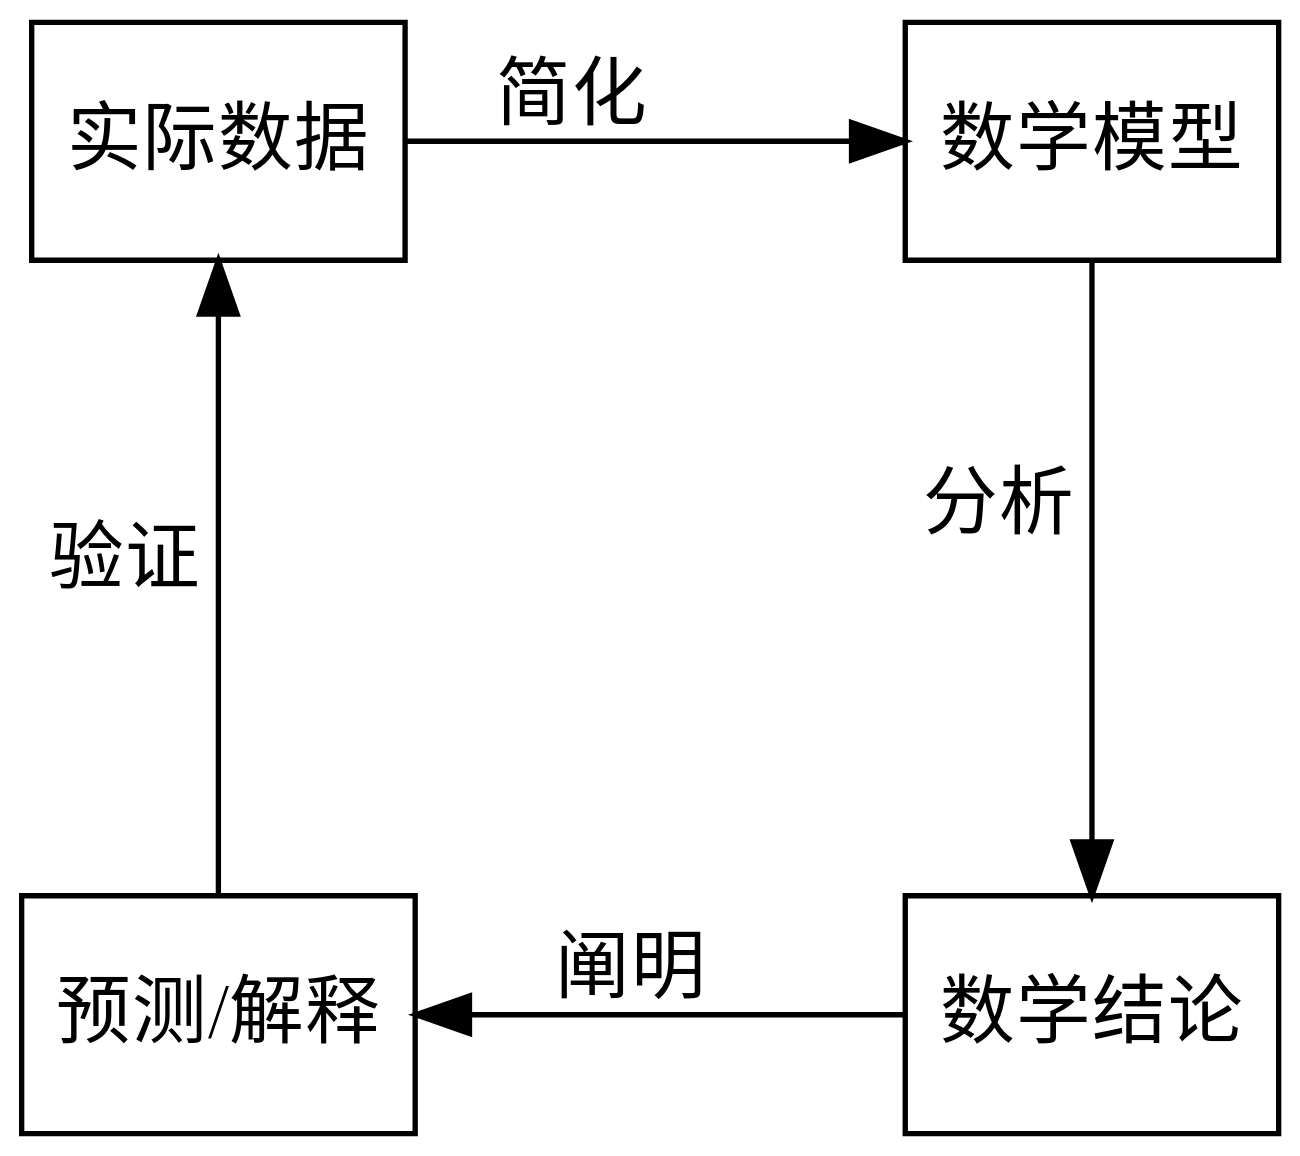
\includegraphics[width=6.5in,height=7in]{index_files/figure-beamer/dot-figure-1.png}
\end{frame}

\begin{frame}{MATLAB}
\phantomsection\label{matlab}
\begin{itemize}
\tightlist
\item
  The MathWorks公司出品的商业数学软件
\item
  用于算法开发、数据可视化、数据分析以及数值计算
\item
  创建用户界面,以及调用其它语言编写的程序
\end{itemize}

\begin{center}
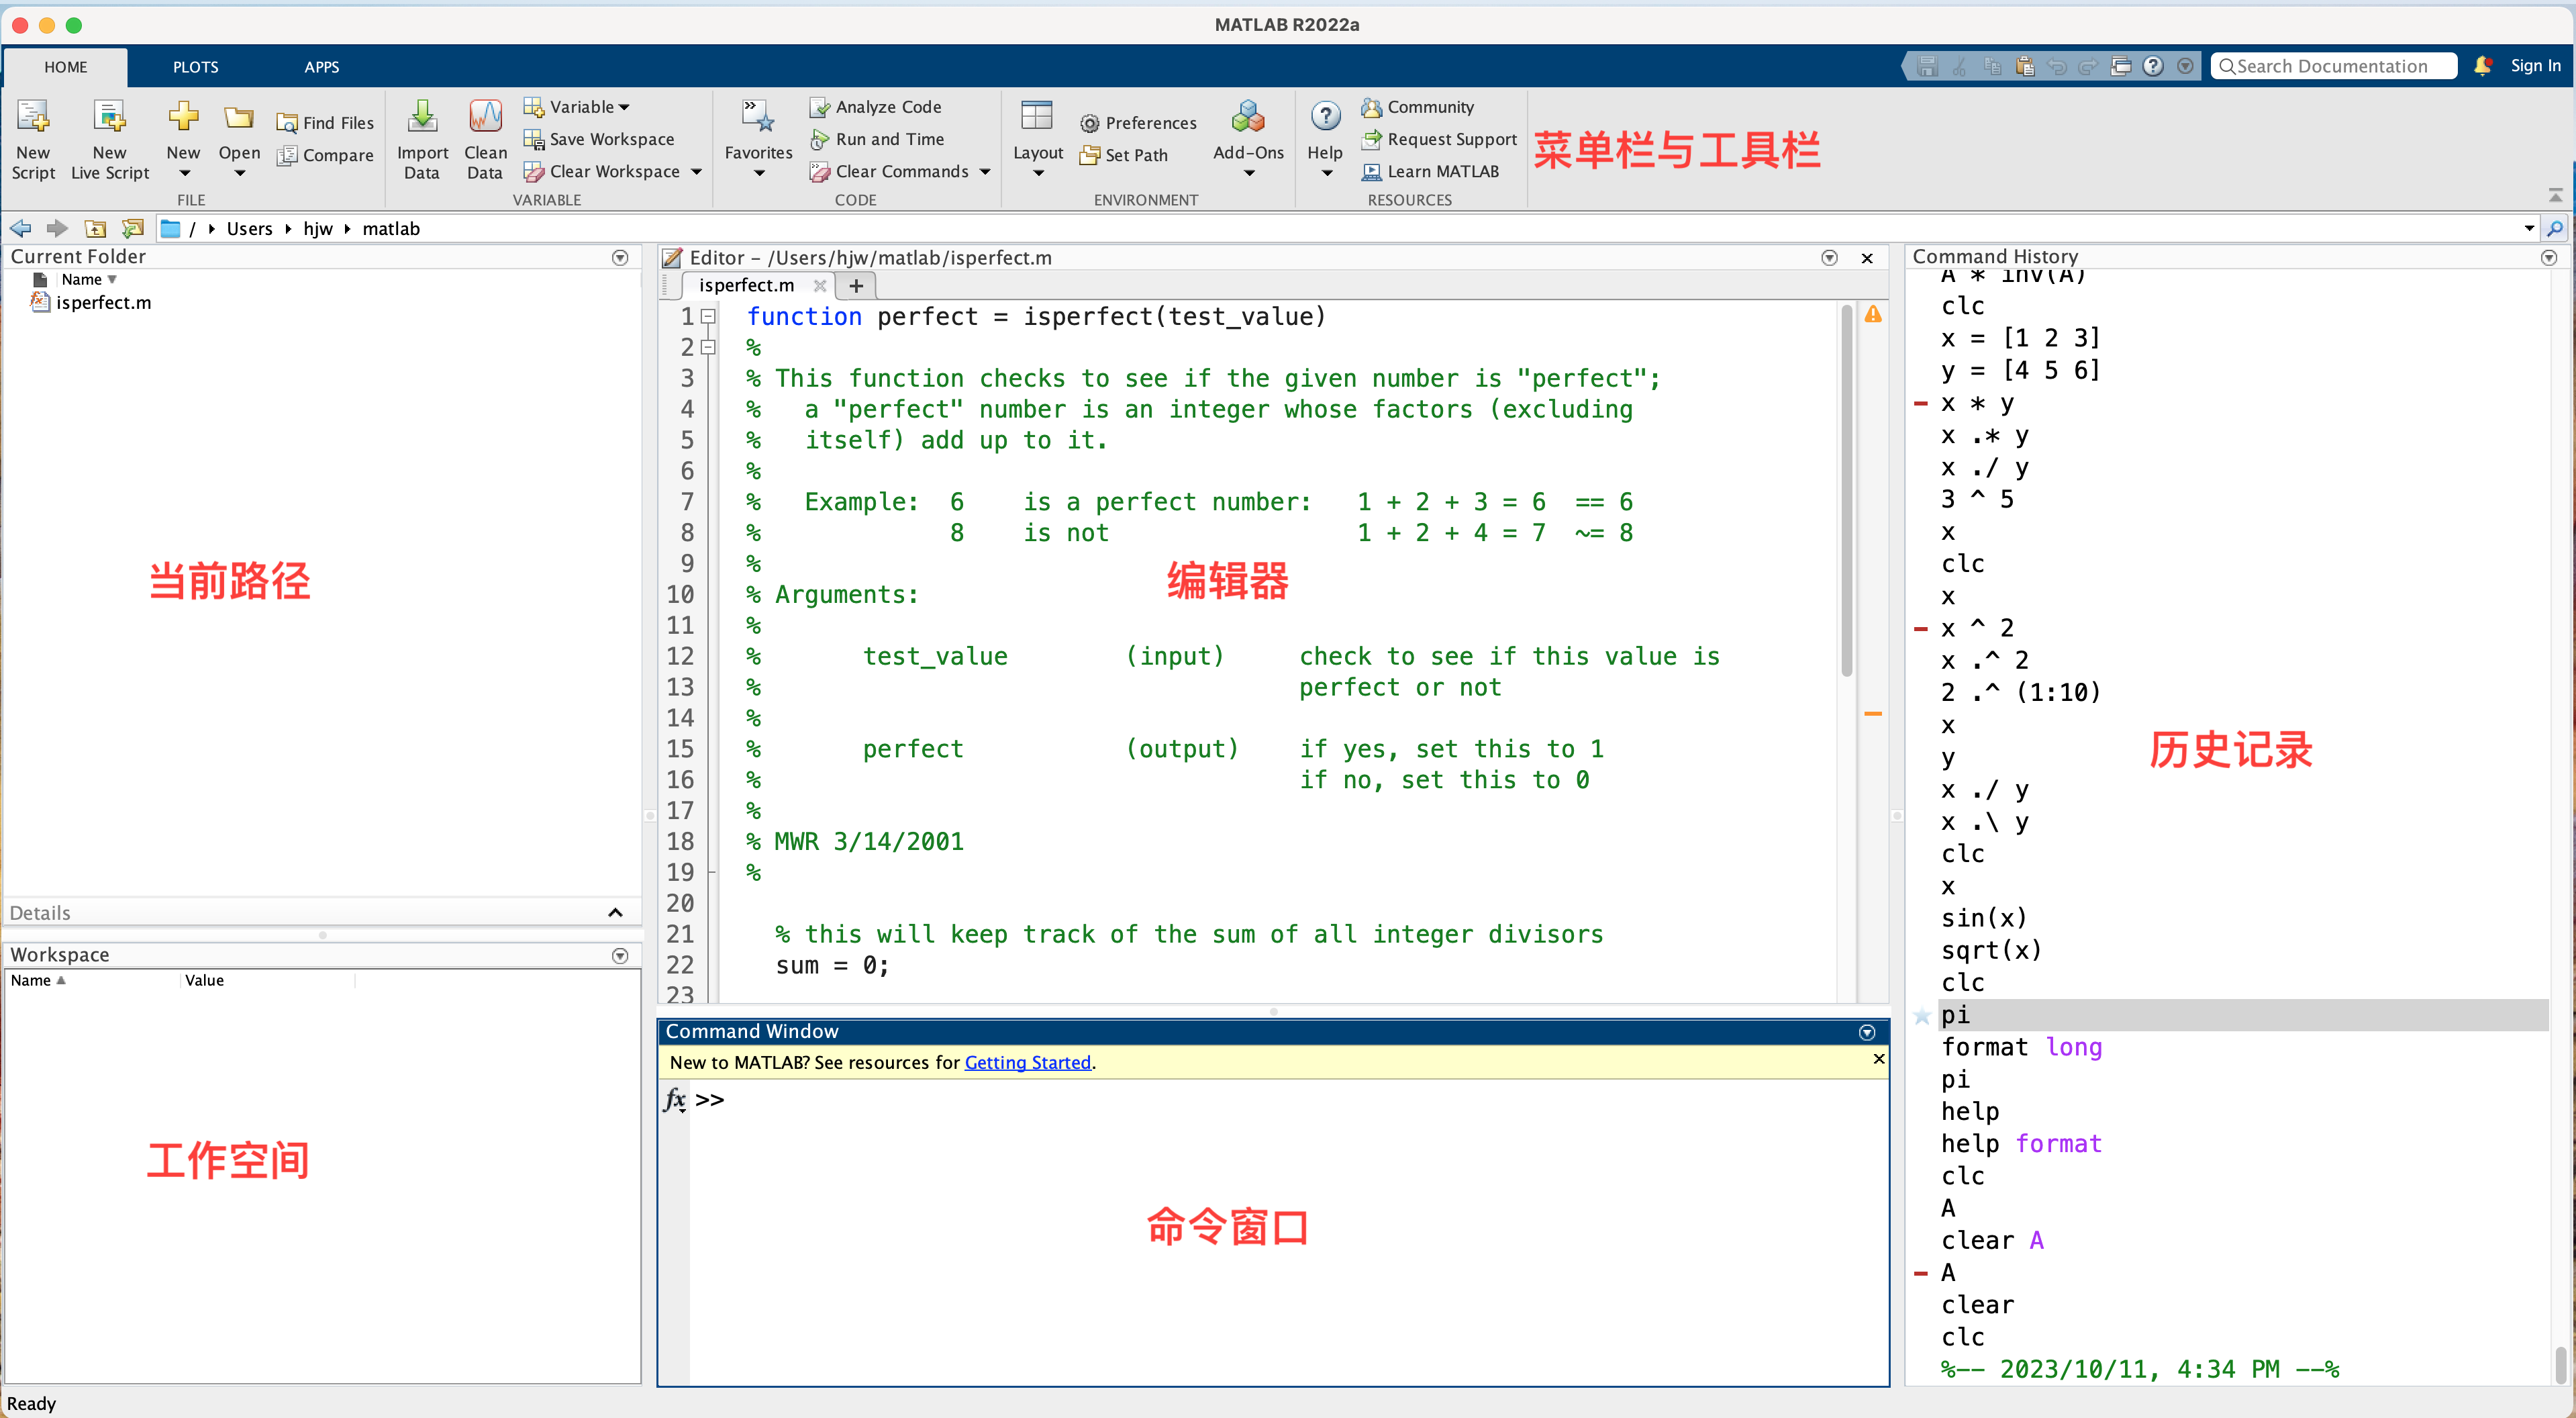
\includegraphics{images/matlab.jpg}
\end{center}
\end{frame}

\begin{frame}{教材及参考资料}
\phantomsection\label{ux6559ux6750ux53caux53c2ux8003ux8d44ux6599}
\begin{itemize}
\tightlist
\item
  \textbf{数学建模(原书第5版), Frank R.Giordano, Willam P.Fox, Steven
  B.Horton, 叶其孝/姜启源译, 机械工业出版社}
\item
  数学模型(第四版), 姜启源/谢金星/叶俊, 高等教育出版社
\item
  数学建模, 杨启帆/谈之奕/何勇, 浙江大学出版社
\item
  数学建模算法与应用, 司守奎/孙玺菁, 国防工业出版社
\item
  MATLAB揭秘, David McMahon著/郑碧波译
\item
  精通MATLAB R2011a, 张志涌, 北京航天航空大学出版社
\end{itemize}
\end{frame}

\begin{frame}{课程安排}
\phantomsection\label{ux8bfeux7a0bux5b89ux6392}
\begin{description}
\tightlist
\item[时间]
16周 = 12课堂 + 4实验
\item[考试]
成绩 = 平时 \(\times\) 30\%+ 期末(闭卷) \(\times\) 70\%
\end{description}
\end{frame}

\begin{frame}{课程概要}
\phantomsection\label{ux8bfeux7a0bux6982ux8981}
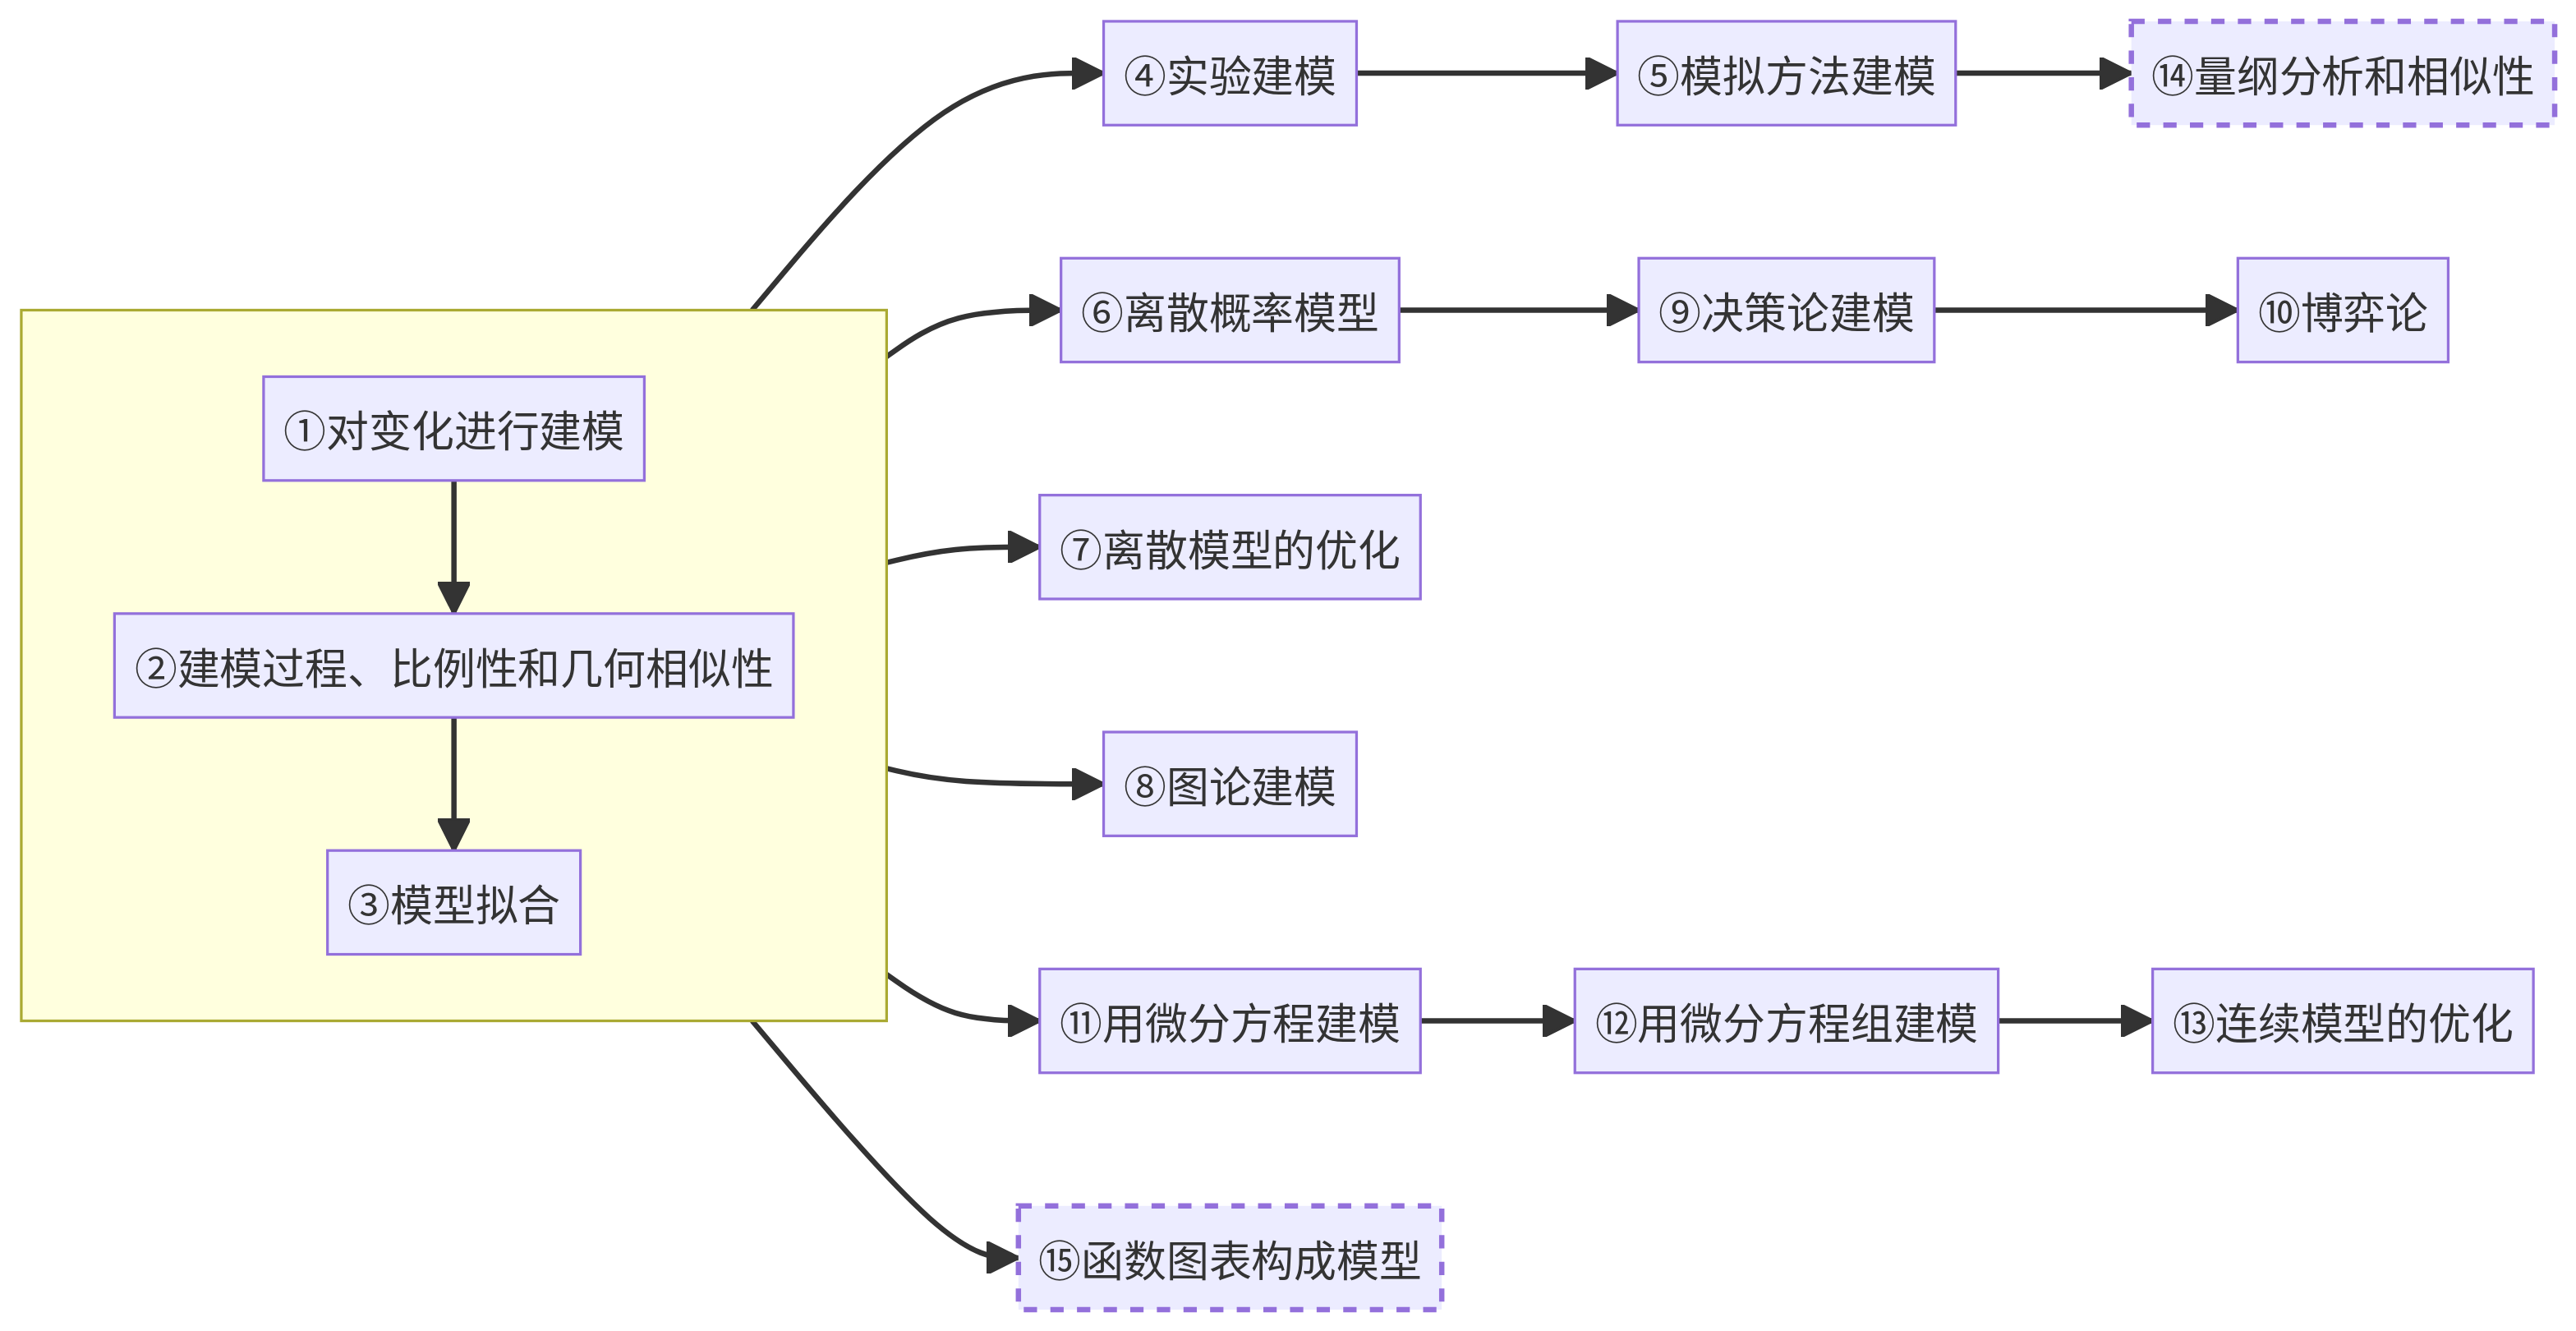
\includegraphics[width=10.08in,height=5.21in]{index_files/figure-beamer/mermaid-figure-1.png}
\end{frame}

\section{第 1 章
对变化进行建模}\label{ux7b2c-1-ux7ae0-ux5bf9ux53d8ux5316ux8fdbux884cux5efaux6a21}

\begin{frame}{弹簧系统}
\phantomsection\label{ux5f39ux7c27ux7cfbux7edf}
\begin{columns}[T]
\begin{column}{0.55\textwidth}
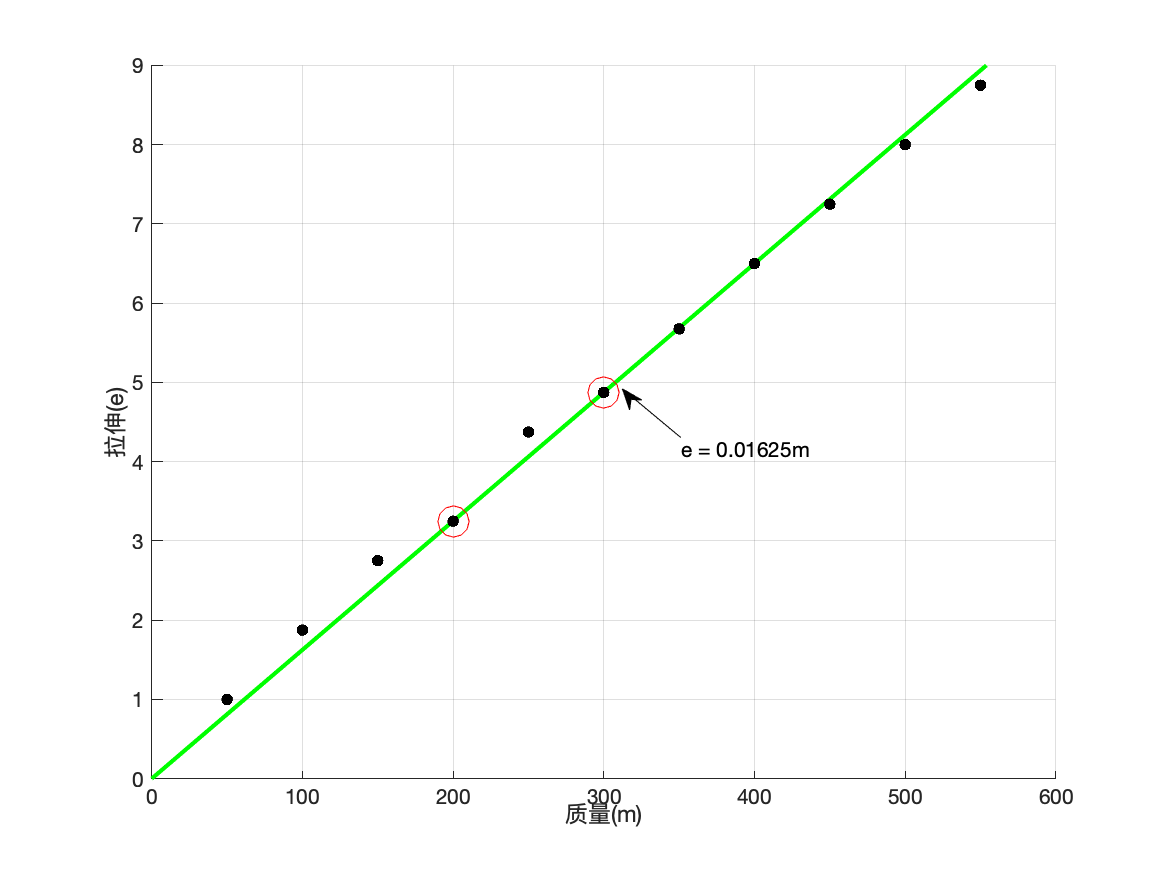
\includegraphics{images/spring_mass.png}
\end{column}

\begin{column}{0.25\textwidth}
\begin{longtable}[]{@{}ll@{}}
\toprule\noalign{}
质量(\(m\)) & 拉伸(\(e\)) \\
\midrule\noalign{}
\endhead
50 & 1.000 \\
100 & 1.875 \\
150 & 2.750 \\
200 & 3.250 \\
250 & 4.375 \\
300 & 4.875 \\
350 & 5.675 \\
400 & 6.500 \\
450 & 7.250 \\
500 & 8.000 \\
550 & 8.750 \\
\bottomrule\noalign{}
\end{longtable}
\end{column}

\begin{column}{0.2\textwidth}
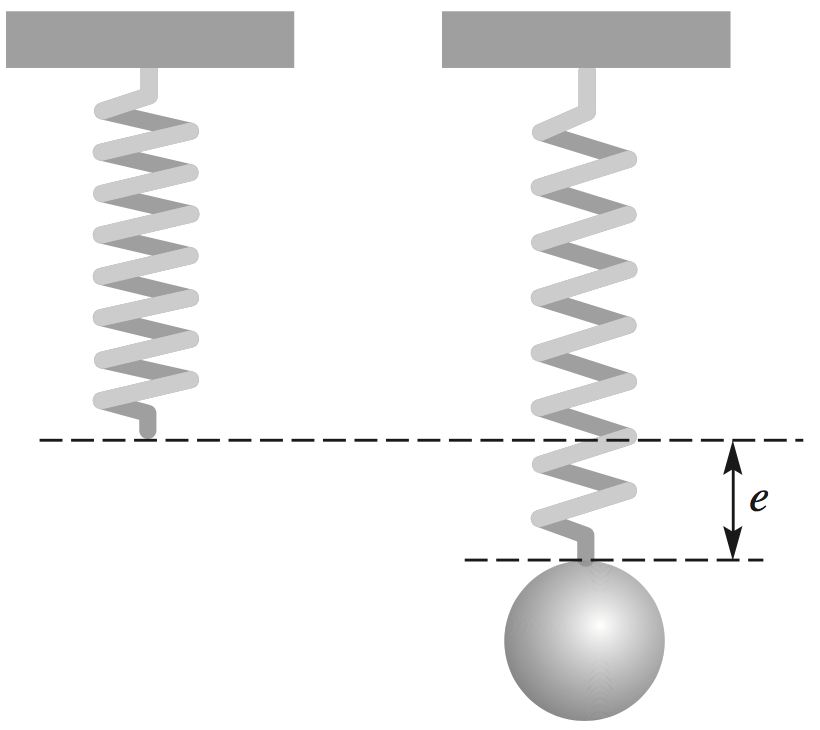
\includegraphics{spring.png}
\end{column}
\end{columns}

\(斜率 = \frac{4.875-3.25}{300-200} = 0.01625\)
\end{frame}

\begin{frame}{对变化进行建模}
\phantomsection\label{ux5bf9ux53d8ux5316ux8fdbux884cux5efaux6a21}
\begin{itemize}
\tightlist
\item
  \[未来值 = 现在值 + 变化\]
\item
  \[变化 = 未来值 - 现在值\]
\end{itemize}

\begin{description}
\tightlist
\item[离散时间]
差分方程(difference equation)
\item[连续时间]
微分方程(第11章)
\end{description}
\end{frame}

\begin{frame}{差分方程}
\phantomsection\label{ux5deeux5206ux65b9ux7a0b}
对于数列\(A = {a_0, a_1, a_2, a_3, \cdots}\), 其一阶差分定义为:

\begin{columns}[T]
\begin{column}{0.4\textwidth}
\[
\Delta a_0 = a_1 - a_0 \\
\Delta a_1 = a_2 - a_1 \\
\Delta a_2 = a_3 - a_2 \\
\Delta a_3 = a_4 - a_3 \\
\cdots \\
\Delta a_n = a_{n+1} - a_n
\]
\end{column}

\begin{column}{0.6\textwidth}
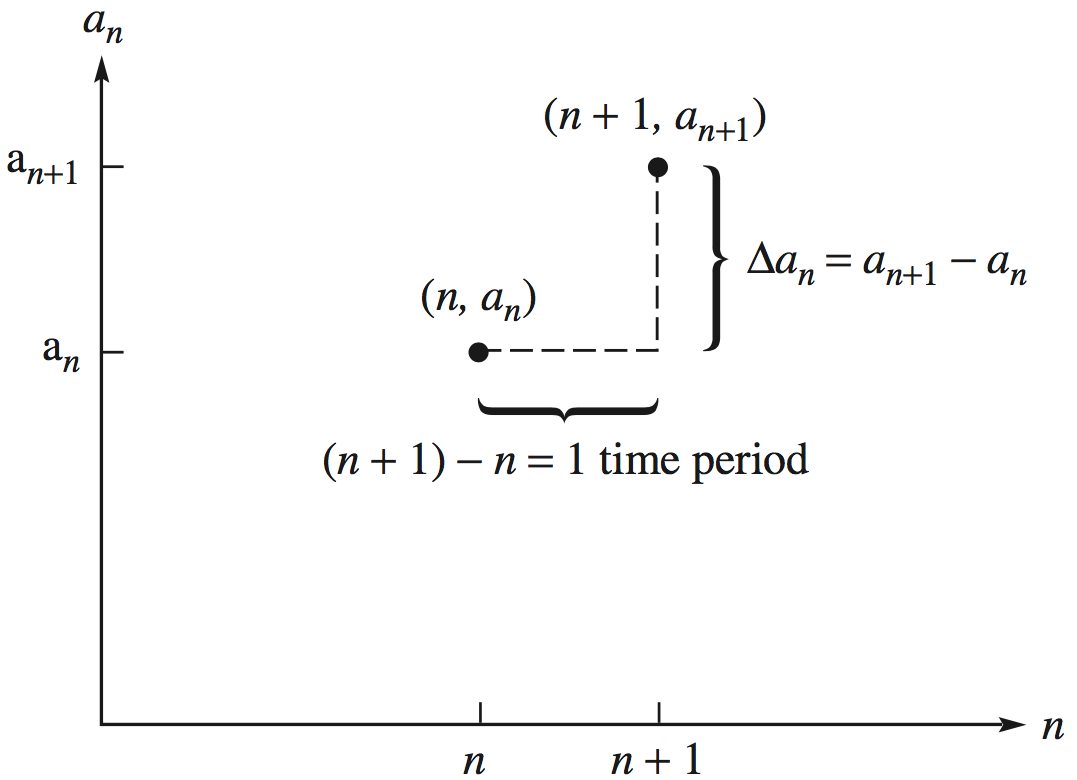
\includegraphics{images/difference.png}
\end{column}
\end{columns}
\end{frame}

\begin{frame}{储蓄问题}
\phantomsection\label{ux50a8ux84c4ux95eeux9898}
考虑本金1000美元,
月利息1\%的储蓄问题\(A = (1000, 1010, 1020.10, 1030.30, ...)\).

\[
\Delta a_0 = a_1 - a_0 = 1010.0 - 1000.0 = 10.0 \\
\Delta a_1 = a_2 - a_1 = 1020.1 - 1010.0 = 10.1 \\
\Delta a_2 = a_3 - a_2 = 1030.3 - 1020.1 = 10.2 \\
\cdots \\
\Delta a_n = a_{n+1} - a_n = 0.01a_n \\
\]

\[
a_{n+1} = a_n + 0.01a_n = 1.01a_n, n = 0, 1, 2, 3 \\
a_0 = 1000
\]

如果每月取出50美元\(\cdots\)

\[\Delta a_n = a_{n+1} - a_n = 0.01a_n - 50\]
\end{frame}

\begin{frame}{如何找出变化?}
\phantomsection\label{ux5982ux4f55ux627eux51faux53d8ux5316}
在多数情况下, 很难象上述例子那样精确表述, 因此我们通过如下步骤找出变化:

\begin{tcolorbox}[enhanced jigsaw, bottomrule=.15mm, bottomtitle=1mm, titlerule=0mm, coltitle=black, arc=.35mm, title=\textcolor{quarto-callout-important-color}{\faExclamation}\hspace{0.5em}{Important}, toptitle=1mm, colbacktitle=quarto-callout-important-color!10!white, colback=white, opacitybacktitle=0.6, colframe=quarto-callout-important-color-frame, rightrule=.15mm, toprule=.15mm, leftrule=.75mm, breakable, left=2mm, opacityback=0]

\begin{enumerate}
\tightlist
\item
  画出变化
\item
  观察变化规律
\item
  用数学术语描述变化
\end{enumerate}

\end{tcolorbox}

变化 = \(\Delta a_n\) = 某个函数\(f\)

对于离散情况:

变化 = \(\Delta a_n\) = \(a_{n+1} - a_n\) = \(f\)(序列中的项, 外部项)
\end{frame}

\begin{frame}{按揭买房}
\phantomsection\label{ux6309ux63edux4e70ux623f}
六年前按揭20年买了一套80000美元的房子, 月供880.87美元并付每月1\%的利息.
问现在还欠银行多少?

\[\Delta b_n = b_{n+1} - b_n = 0.01b_n - 880.87\]

求解下列方程即可:

\[
\begin{align*}
b_{n+1} &= 1.01b_n - 880.87 \\
b_0 &= 80000
\end{align*}
\]

\[B = (80000, 79919.13, 79837.45, \cdots)\]
\end{frame}

\begin{frame}{按揭买房}
\phantomsection\label{ux6309ux63edux4e70ux623f-1}
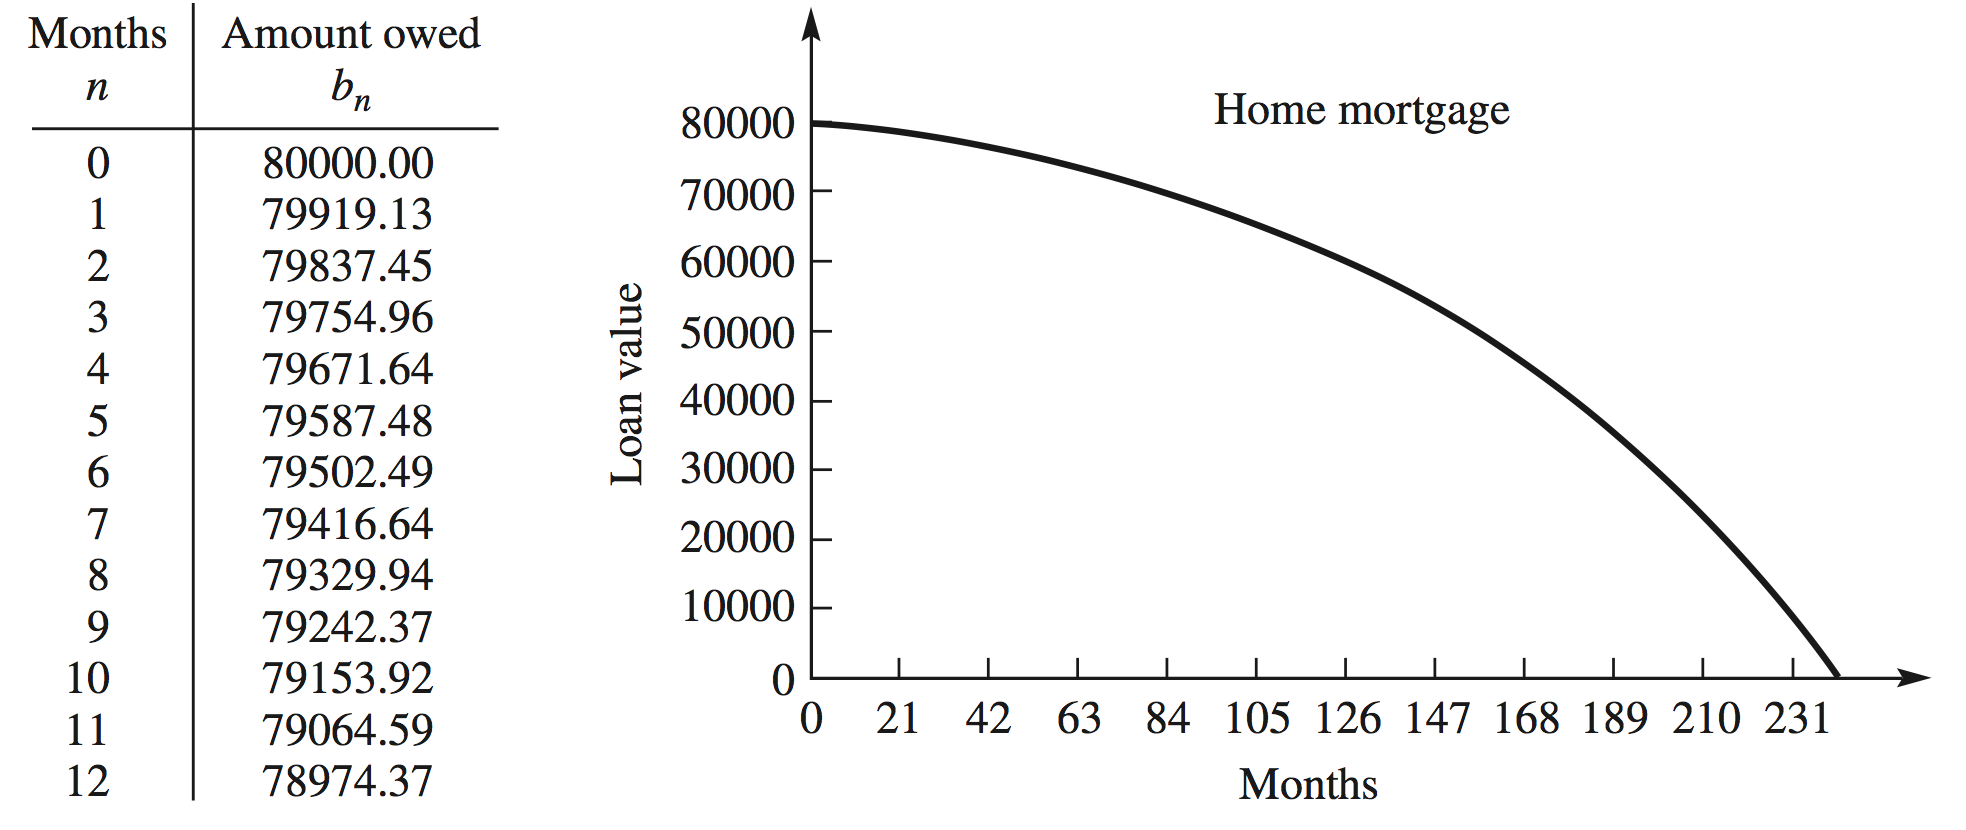
\includegraphics{mort.png}
\end{frame}

\begin{frame}{用差分方程来近似变化}
\phantomsection\label{ux7528ux5deeux5206ux65b9ux7a0bux6765ux8fd1ux4f3cux53d8ux5316}
\begin{itemize}
\item
  变化 = \(\Delta a_n\) = 某个函数\(f\)
\item
  离散变化与连续变化
\item
  模型的细化: 生、死、资源
\end{itemize}
\end{frame}

\begin{frame}{酵母培养 -- 找出模型}
\phantomsection\label{ux9175ux6bcdux57f9ux517b-ux627eux51faux6a21ux578b}
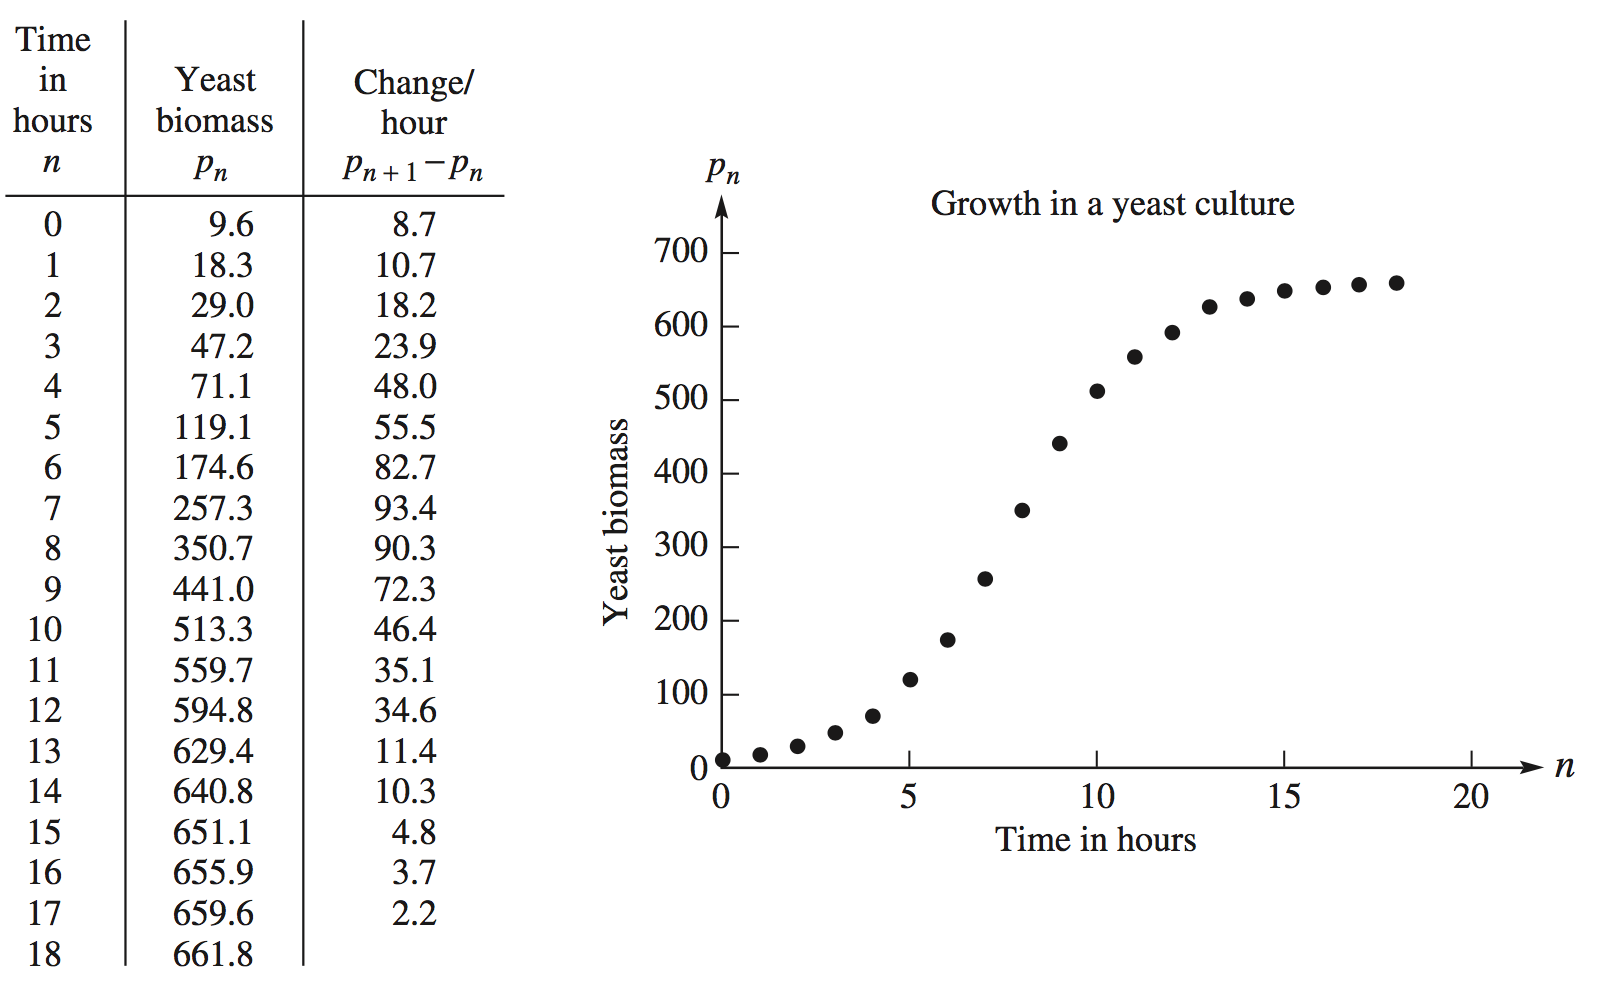
\includegraphics{yeast.png}

\[\Delta p_n = p_{n+1} - p_n = k(665 - p_n)p_n\]
\end{frame}

\begin{frame}{酵母培养 -- 模型数值求解}
\phantomsection\label{ux9175ux6bcdux57f9ux517b-ux6a21ux578bux6570ux503cux6c42ux89e3}
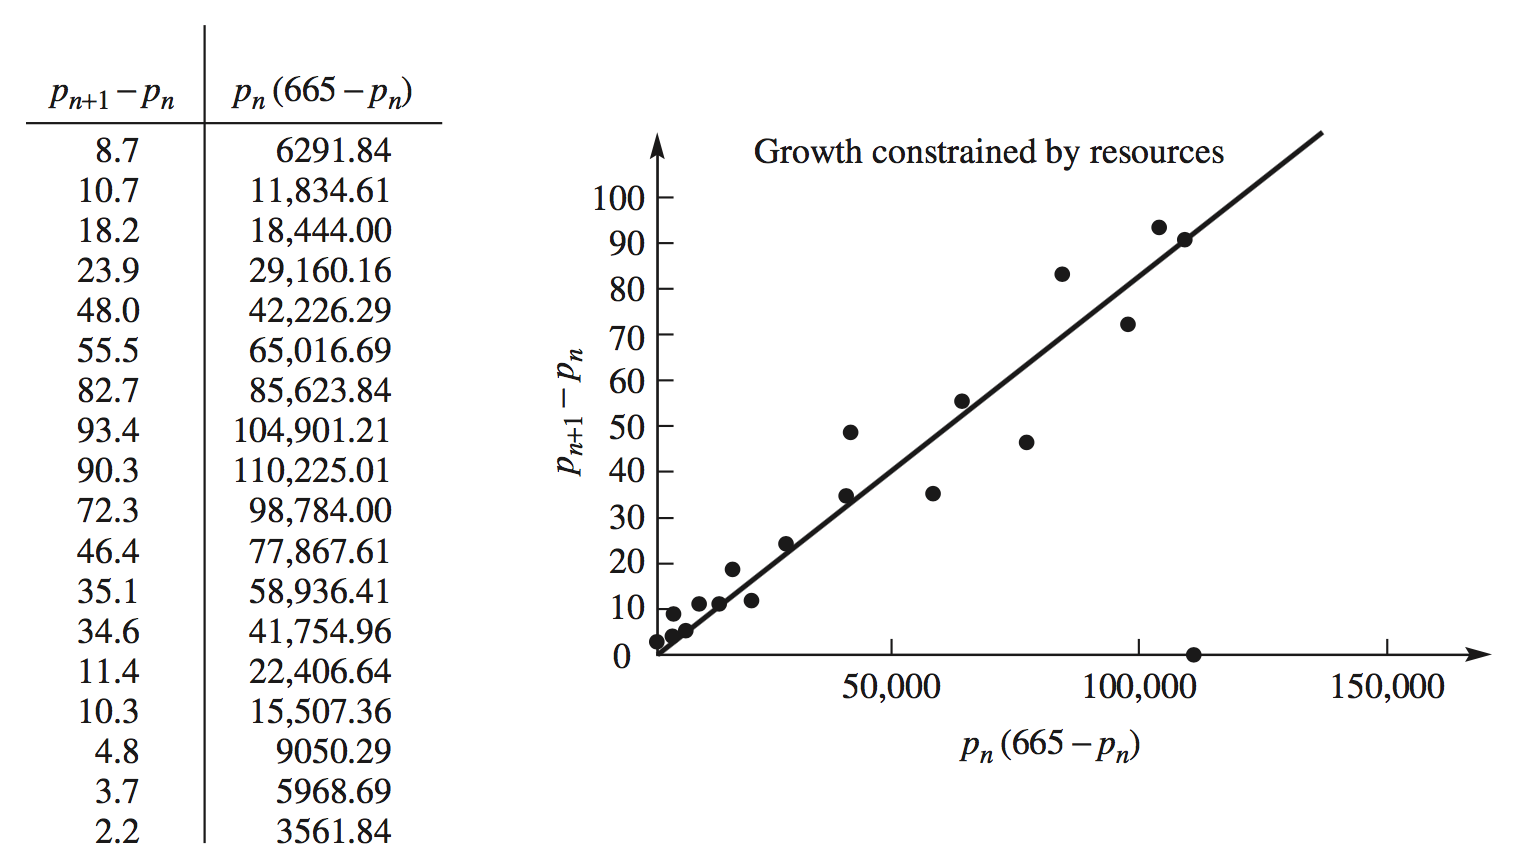
\includegraphics{yeast-fit.png}

\[k \approx 0.00082\] \[p_{n+1} = p_n + 0.00082(665 - p_n)p_n\]
\end{frame}

\begin{frame}{酵母培养 -- 模型验证}
\phantomsection\label{ux9175ux6bcdux57f9ux517b-ux6a21ux578bux9a8cux8bc1}
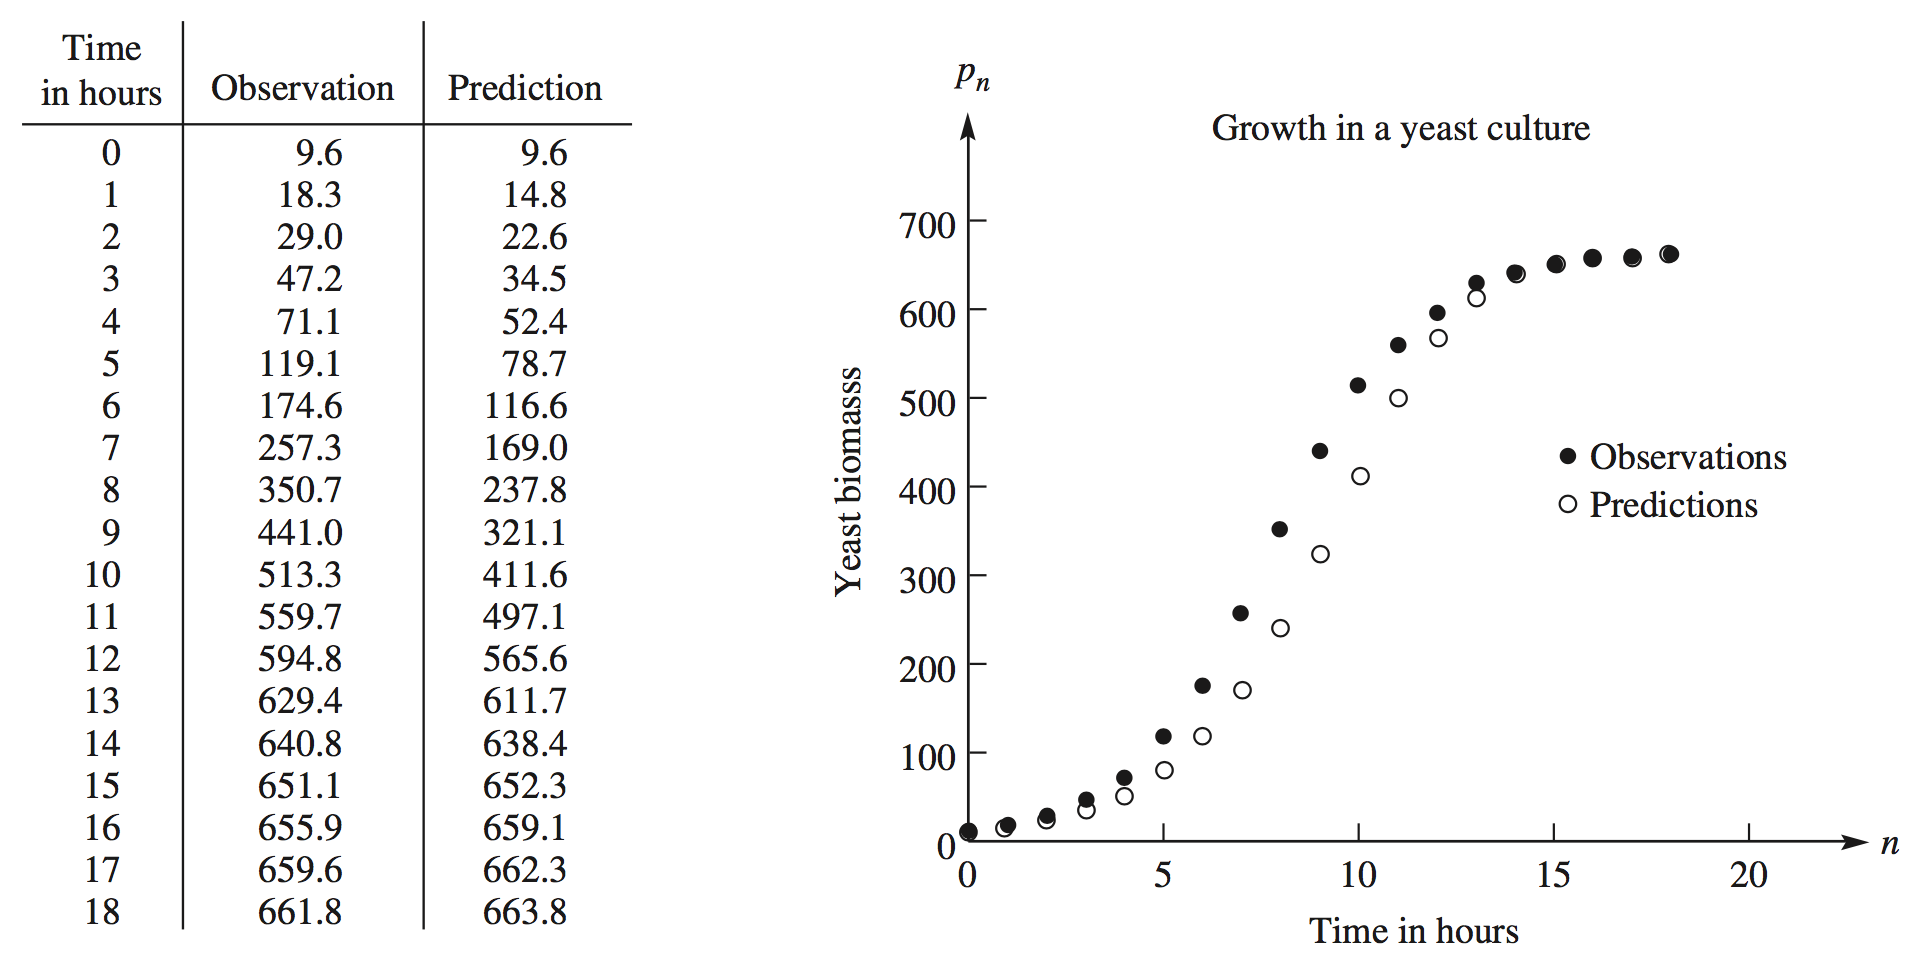
\includegraphics{yeast-verify.png}

\[p_{n+1} = p_n + 0.00082(665 - p_n)p_n\]

思考: 看书上例2传染病传播模型, 考虑如何为该模型加入其它因素?
\end{frame}

\begin{frame}{地高辛在血流中的变化}
\phantomsection\label{ux5730ux9ad8ux8f9bux5728ux8840ux6d41ux4e2dux7684ux53d8ux5316}
\begin{longtable}[]{@{}
  >{\raggedright\arraybackslash}p{(\columnwidth - 18\tabcolsep) * \real{0.1647}}
  >{\raggedright\arraybackslash}p{(\columnwidth - 18\tabcolsep) * \real{0.0941}}
  >{\raggedright\arraybackslash}p{(\columnwidth - 18\tabcolsep) * \real{0.0941}}
  >{\raggedright\arraybackslash}p{(\columnwidth - 18\tabcolsep) * \real{0.0941}}
  >{\raggedright\arraybackslash}p{(\columnwidth - 18\tabcolsep) * \real{0.0941}}
  >{\raggedright\arraybackslash}p{(\columnwidth - 18\tabcolsep) * \real{0.0941}}
  >{\raggedright\arraybackslash}p{(\columnwidth - 18\tabcolsep) * \real{0.0941}}
  >{\raggedright\arraybackslash}p{(\columnwidth - 18\tabcolsep) * \real{0.0941}}
  >{\raggedright\arraybackslash}p{(\columnwidth - 18\tabcolsep) * \real{0.0941}}
  >{\raggedright\arraybackslash}p{(\columnwidth - 18\tabcolsep) * \real{0.0824}}@{}}
\toprule\noalign{}
\begin{minipage}[b]{\linewidth}\raggedright
n
\end{minipage} & \begin{minipage}[b]{\linewidth}\raggedright
0
\end{minipage} & \begin{minipage}[b]{\linewidth}\raggedright
1
\end{minipage} & \begin{minipage}[b]{\linewidth}\raggedright
2
\end{minipage} & \begin{minipage}[b]{\linewidth}\raggedright
3
\end{minipage} & \begin{minipage}[b]{\linewidth}\raggedright
4
\end{minipage} & \begin{minipage}[b]{\linewidth}\raggedright
5
\end{minipage} & \begin{minipage}[b]{\linewidth}\raggedright
6
\end{minipage} & \begin{minipage}[b]{\linewidth}\raggedright
7
\end{minipage} & \begin{minipage}[b]{\linewidth}\raggedright
8
\end{minipage} \\
\midrule\noalign{}
\endhead
\(a_n\) & 0.5 & 0.345 & 0.238 & 0.164 & 0.113 & 0.078 & 0.054 & 0.037 &
0.026 \\
\(\Delta a_n\) & -0.155 & -0.107 & -0.074 & -0.051 & -0.035 & -0.024 &
-0.017 & -0.011 & \\
\bottomrule\noalign{}
\end{longtable}

\begin{columns}[T]
\begin{column}{0.5\textwidth}
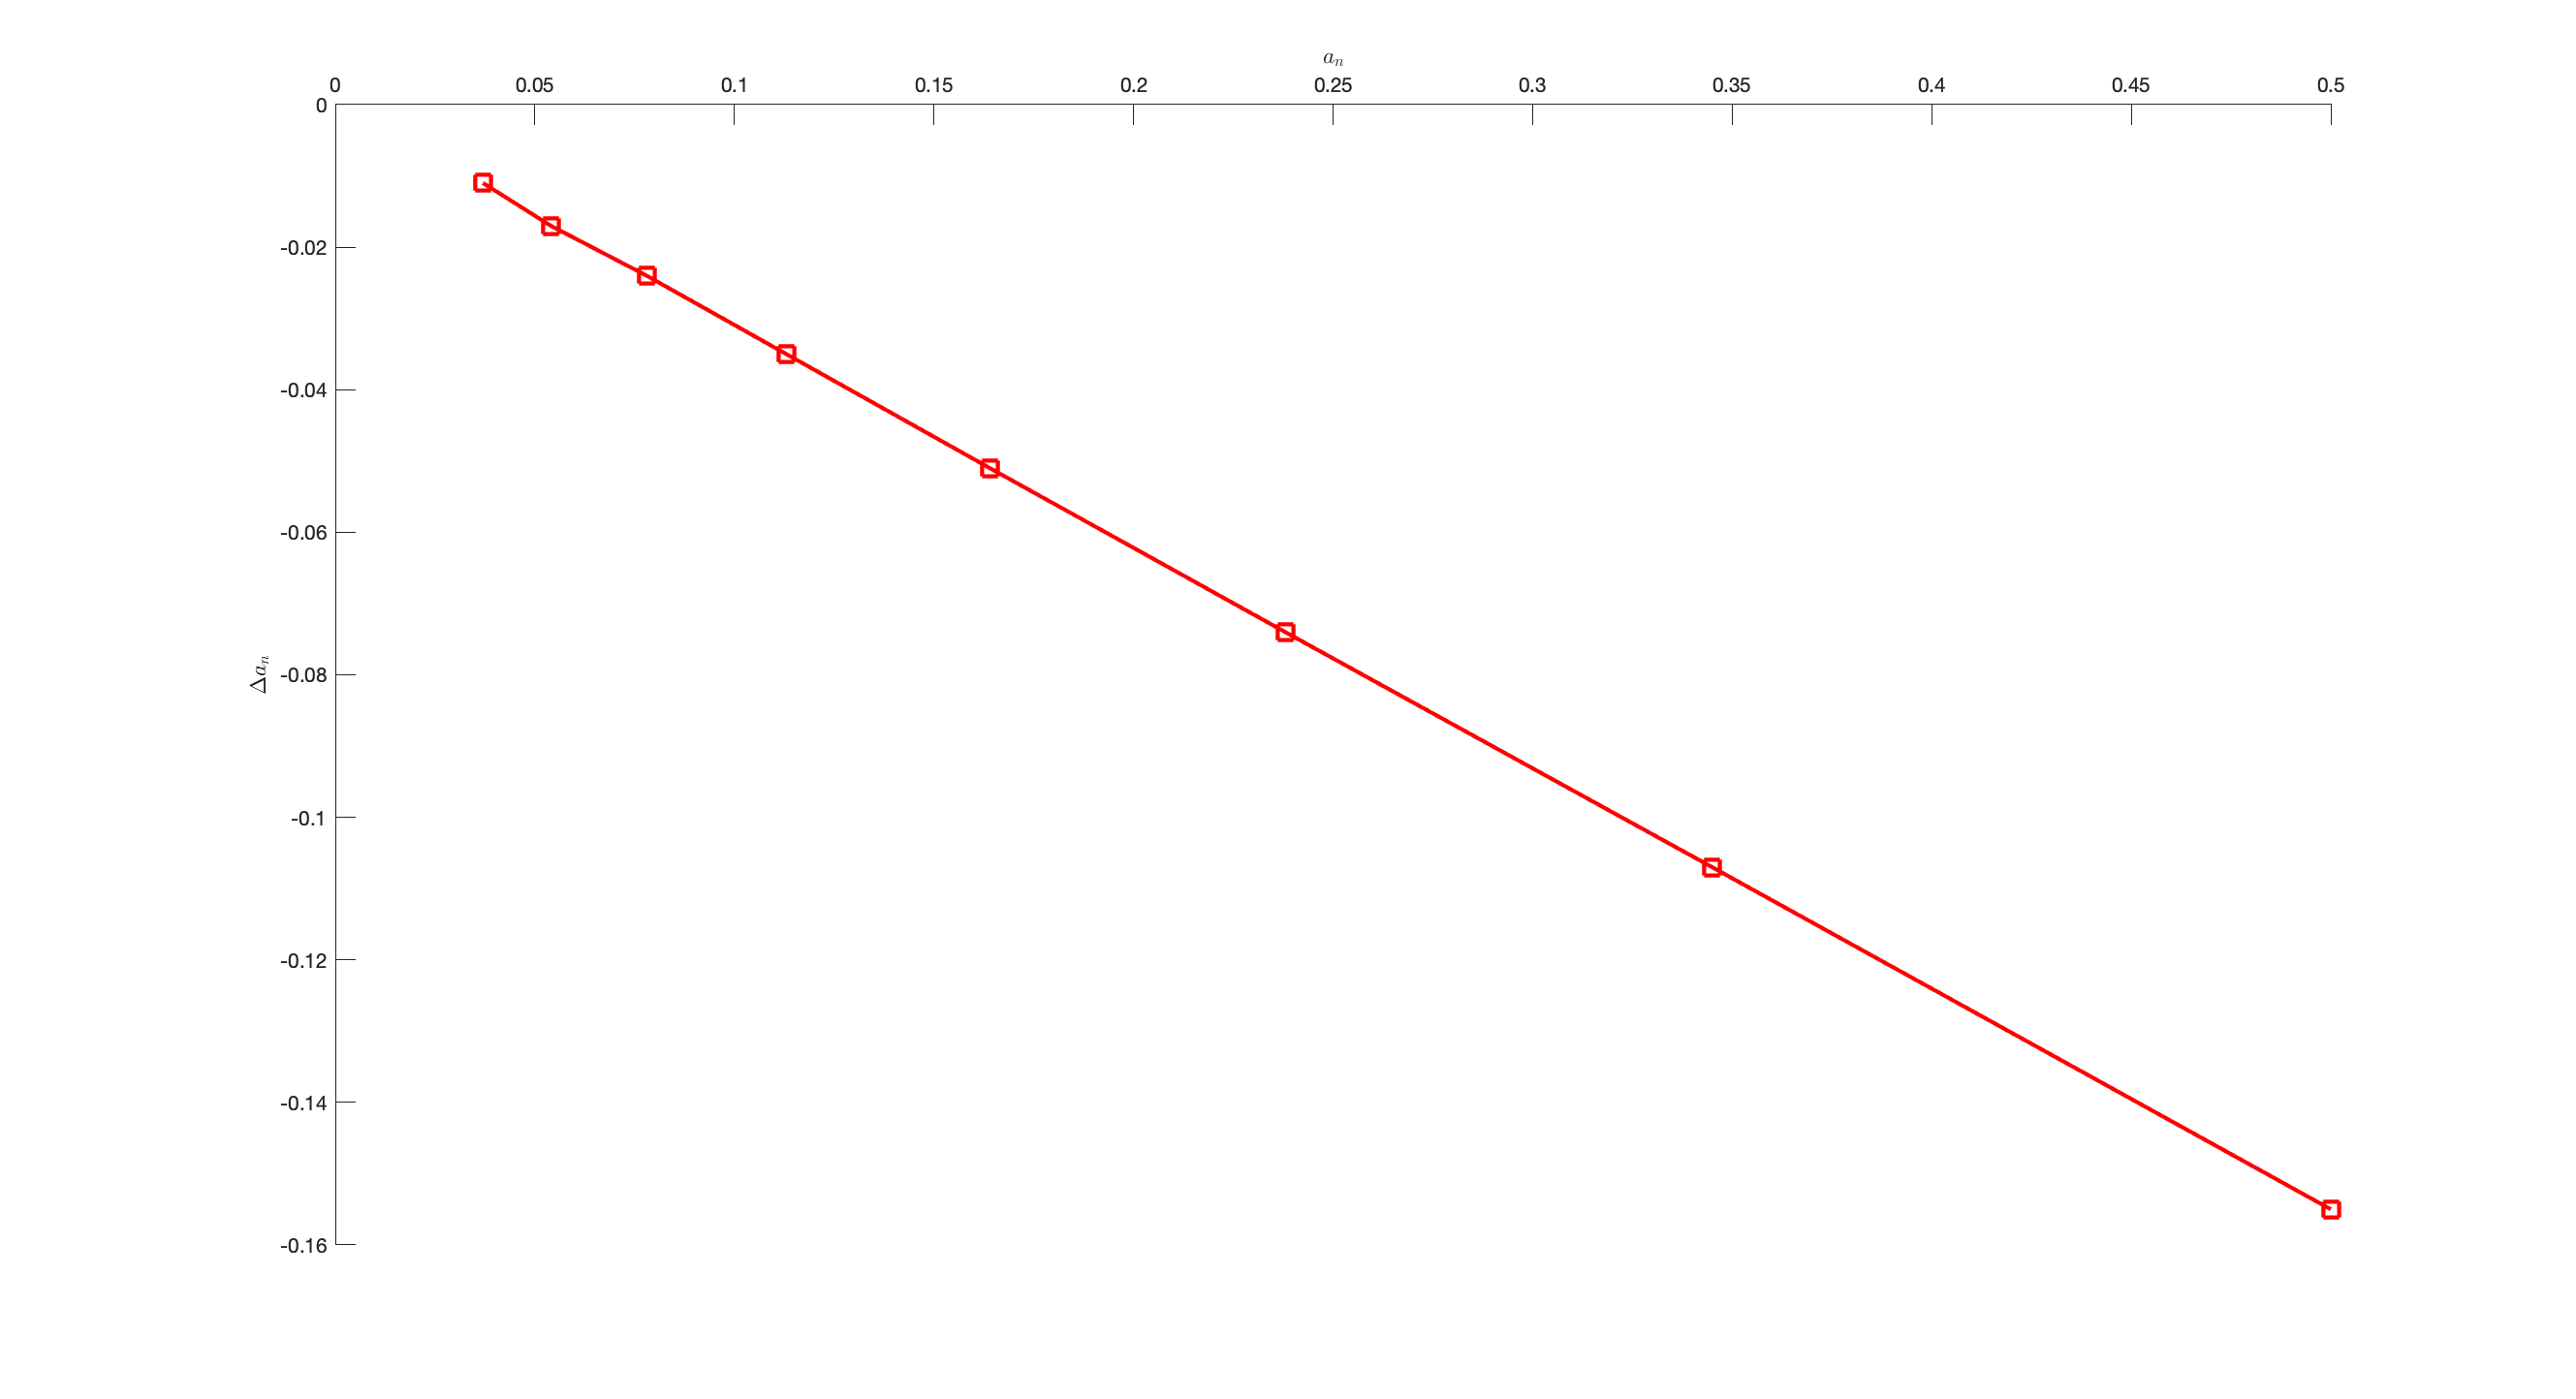
\includegraphics{images/digoxin.png}
\end{column}

\begin{column}{0.5\textwidth}
\[
\Delta a_n = -0.31a_n \\
a_{n+1} -  a_n = -0.31a_n \\
a_{n+1} = 0.69a_n
\]
\end{column}
\end{columns}
\end{frame}

\begin{frame}{动态系统的解法 -- 猜测}
\phantomsection\label{ux52a8ux6001ux7cfbux7edfux7684ux89e3ux6cd5-ux731cux6d4b}
存款问题: \(a_{n+1} = 1.01a_n, a_0 = 1000\)

\[
\begin{align*}
a_1 &= 1010.0 = 1.01(1000)\\
a_2 &= 1020.1 = 1.01(1010) = 1.01^2 (1000)\\
a_3 &= 1030.3 = 1.01(1020.1) = 1.01^3 (1000)\\
a_4 &= 1040.6 = 1.01(1030.3) = 1.01^4 (1000)
\end{align*}
\]

\begin{columns}[T]
\begin{column}{0.6\textwidth}
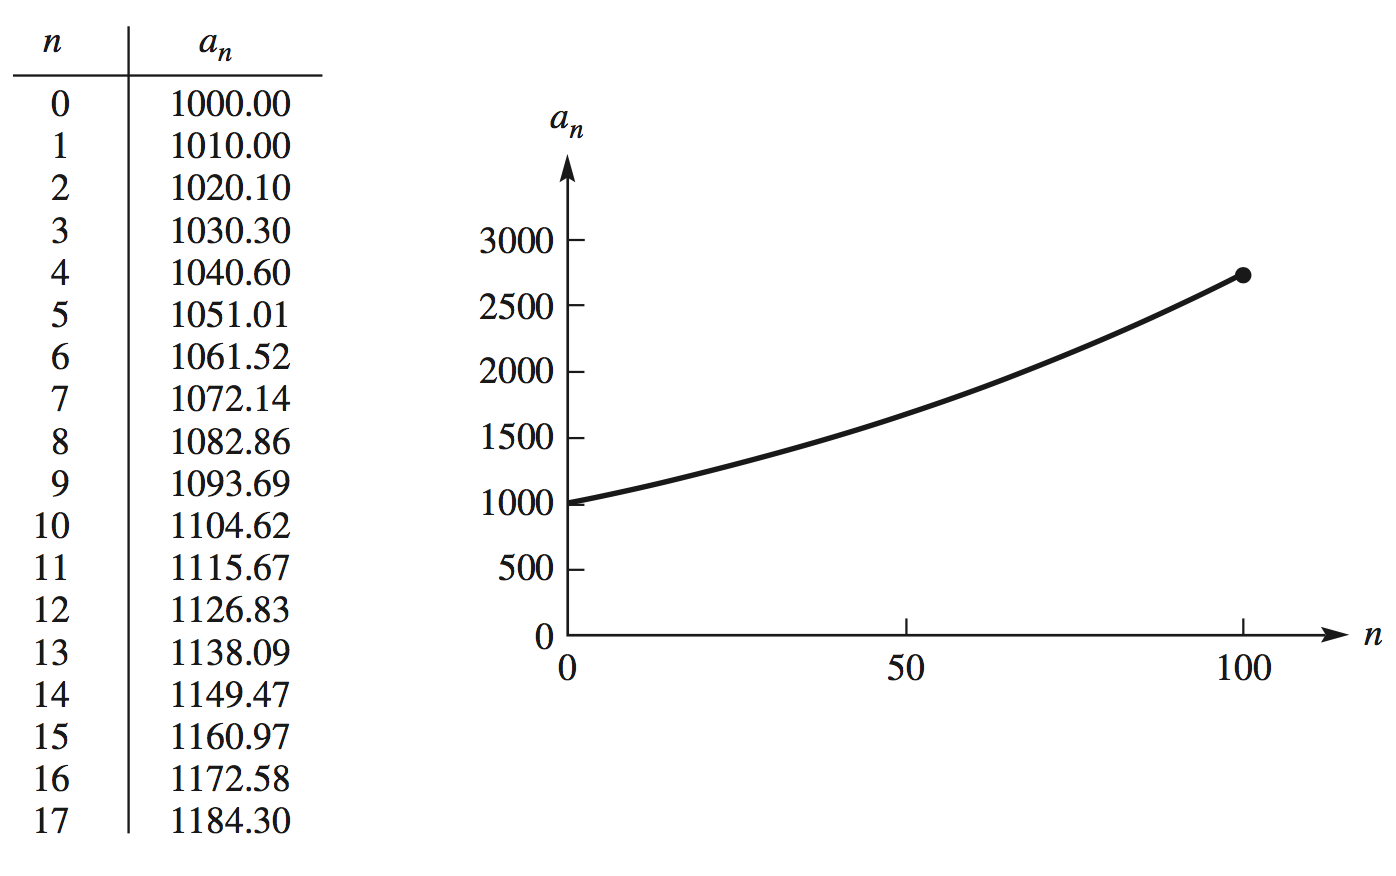
\includegraphics{saving.png}
\end{column}
\end{columns}
\end{frame}

\begin{frame}{动态系统的解法 -- 猜测}
\phantomsection\label{ux52a8ux6001ux7cfbux7edfux7684ux89e3ux6cd5-ux731cux6d4b-1}
猜测: \(a_k = 1.01^k(1000)\) 验证、结论: \ldots{}

\begin{tcolorbox}[enhanced jigsaw, bottomrule=.15mm, bottomtitle=1mm, titlerule=0mm, coltitle=black, arc=.35mm, title=\textcolor{quarto-callout-tip-color}{\faLightbulb}\hspace{0.5em}{Tip}, toptitle=1mm, colbacktitle=quarto-callout-tip-color!10!white, colback=white, opacitybacktitle=0.6, colframe=quarto-callout-tip-color-frame, rightrule=.15mm, toprule=.15mm, leftrule=.75mm, breakable, left=2mm, opacityback=0]

推测法的一般步骤

\begin{enumerate}
\item
  观察模式
\item
  猜测动力系统的形式
\item
  用带入法来测试该猜测
\item
  接受或拒绝该推测:取决于代入和代数运算后结果是否满足该动力系统。
\end{enumerate}

\end{tcolorbox}

推论: 形式为\(a_{n+1} = ra_n\)的动态系统的解为\(a_k = r^k a_0\).
\end{frame}

\begin{frame}{\(a_{n+1}=ra_n\)}
\phantomsection\label{a_n1ra_n}
\(r = ?\)

\begin{columns}[T]
\begin{column}{0.4\textwidth}
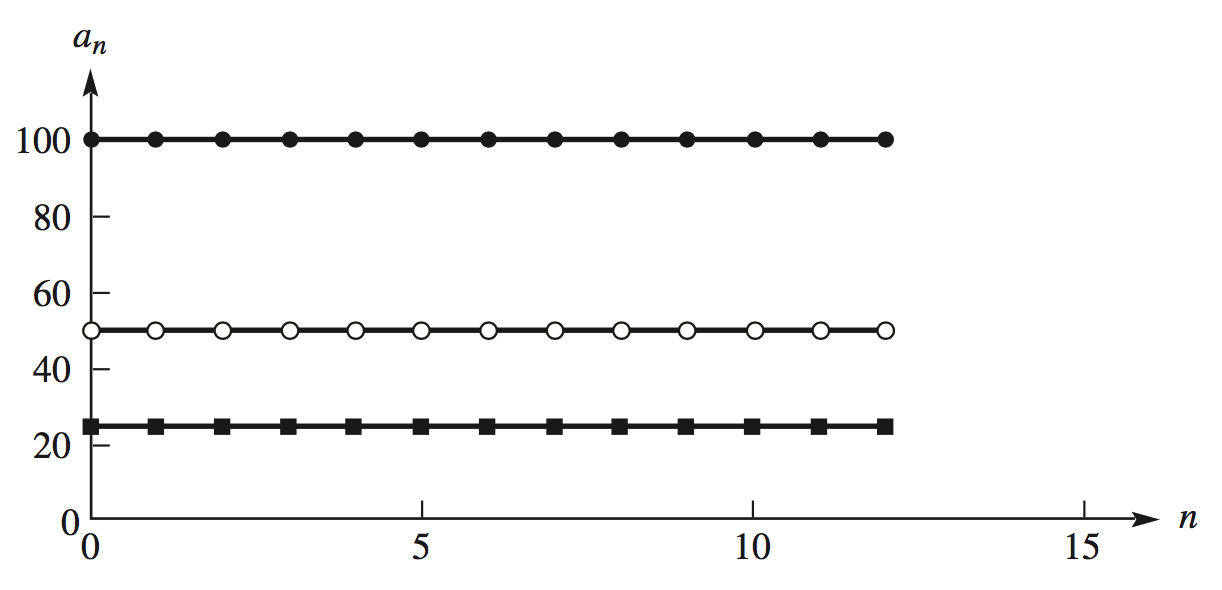
\includegraphics{r0.png} 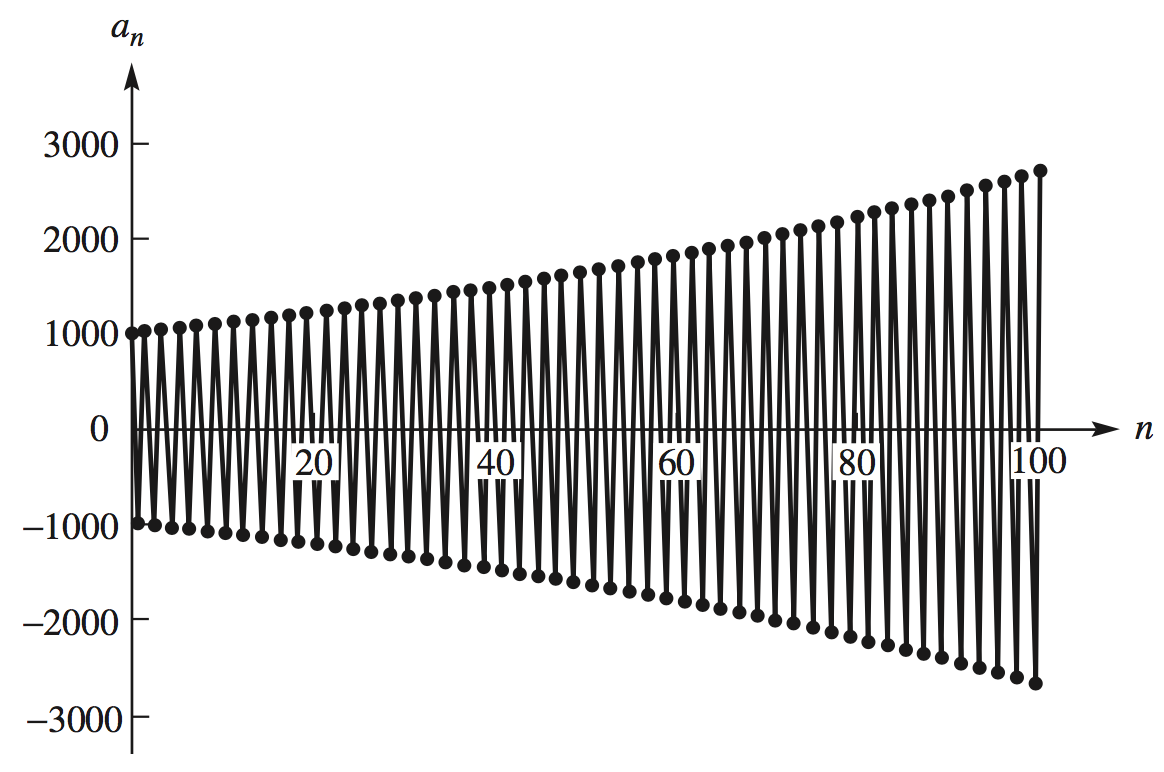
\includegraphics{rn.png}
\end{column}

\begin{column}{0.2\textwidth}
\end{column}

\begin{column}{0.4\textwidth}
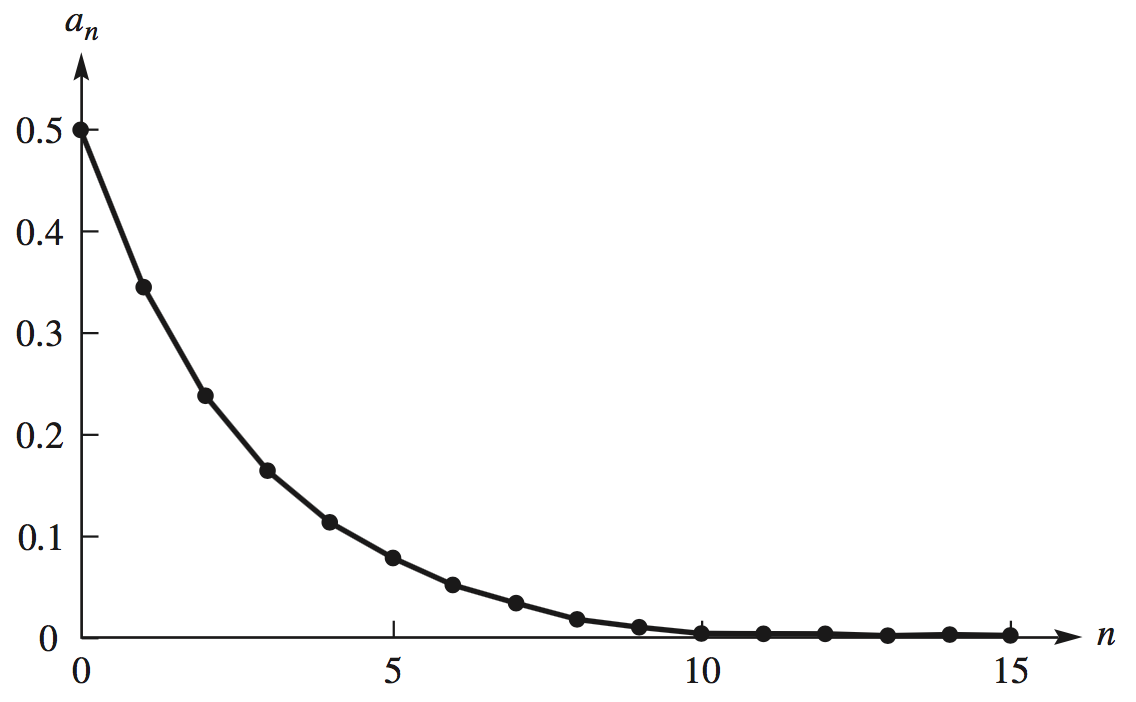
\includegraphics{rf.png} 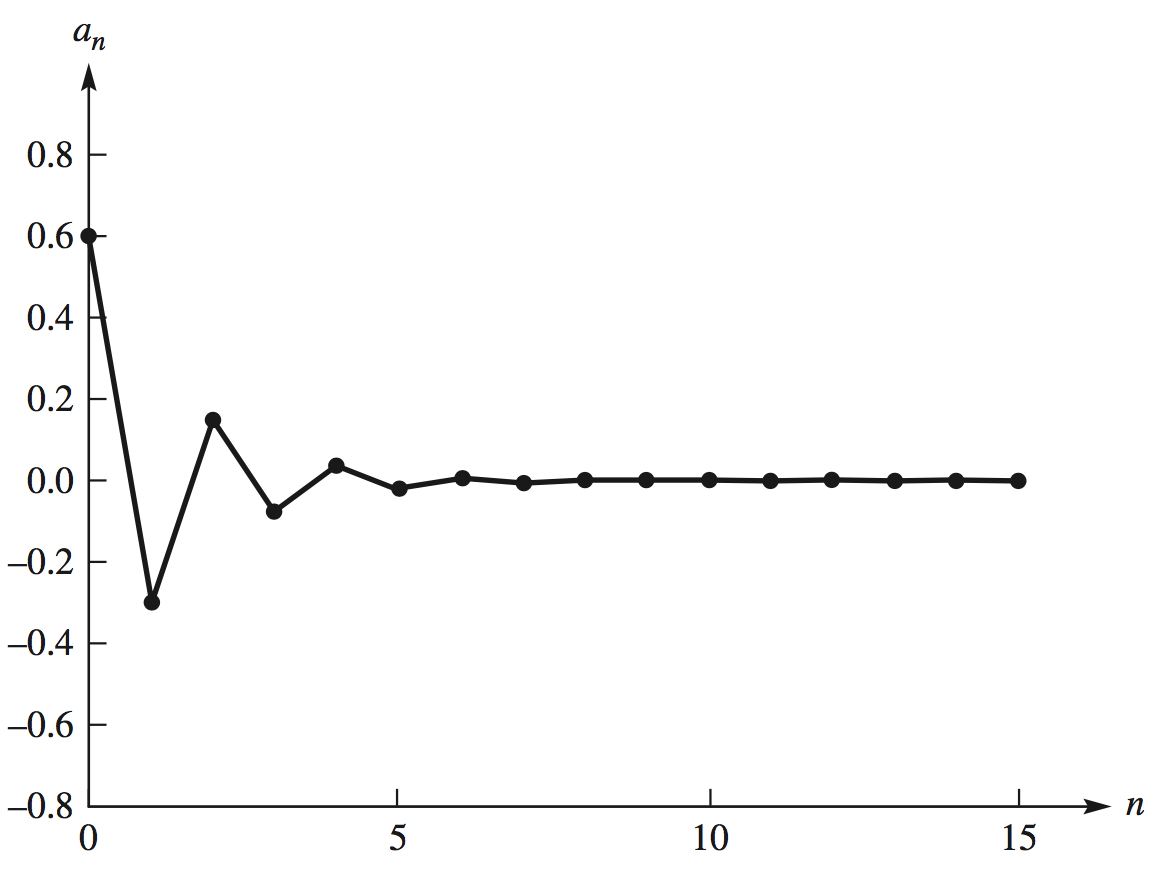
\includegraphics{rnf.png}
\end{column}
\end{columns}
\end{frame}

\begin{frame}{\(a_{n+1}=ra_n + b\)}
\phantomsection\label{a_n1ra_n-b}
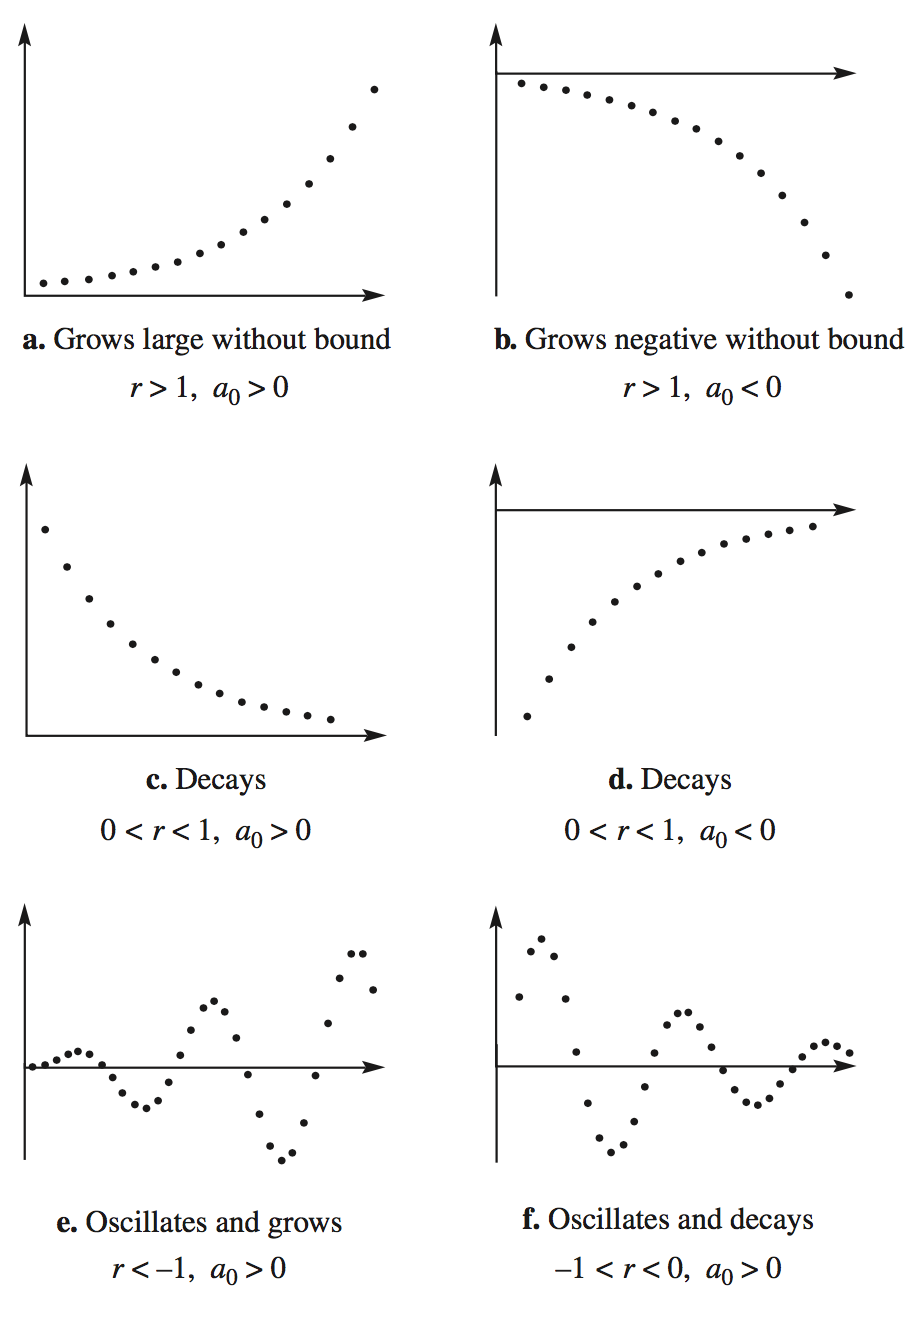
\includegraphics[width=0.4\textwidth,height=\textheight]{rb.png}
\end{frame}

\begin{frame}{不动点(平衡点)}
\phantomsection\label{ux4e0dux52a8ux70b9ux5e73ux8861ux70b9}
\begin{figure}[H]

{\centering 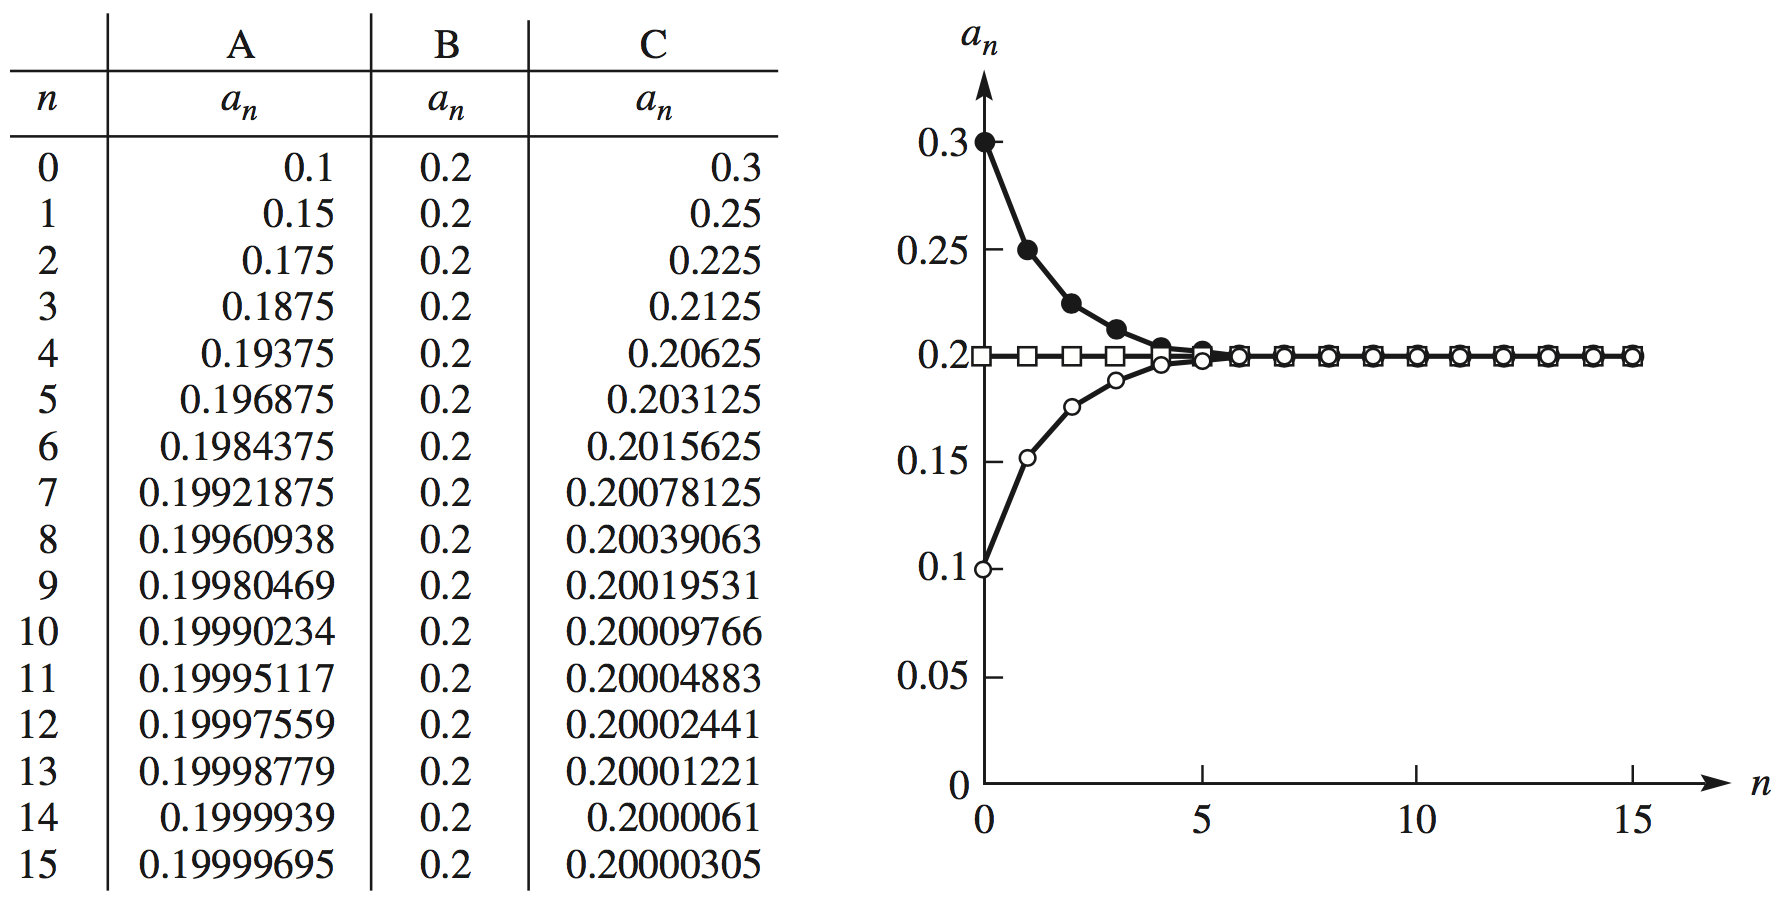
\includegraphics{fixedpoint.png}

}

\caption{Digoxin浓度变化}

\end{figure}%
\end{frame}

\begin{frame}{不动点}
\phantomsection\label{ux4e0dux52a8ux70b9}
\[a_{n+1} = 1.01a_n -1000\]

\begin{figure}[H]

{\centering 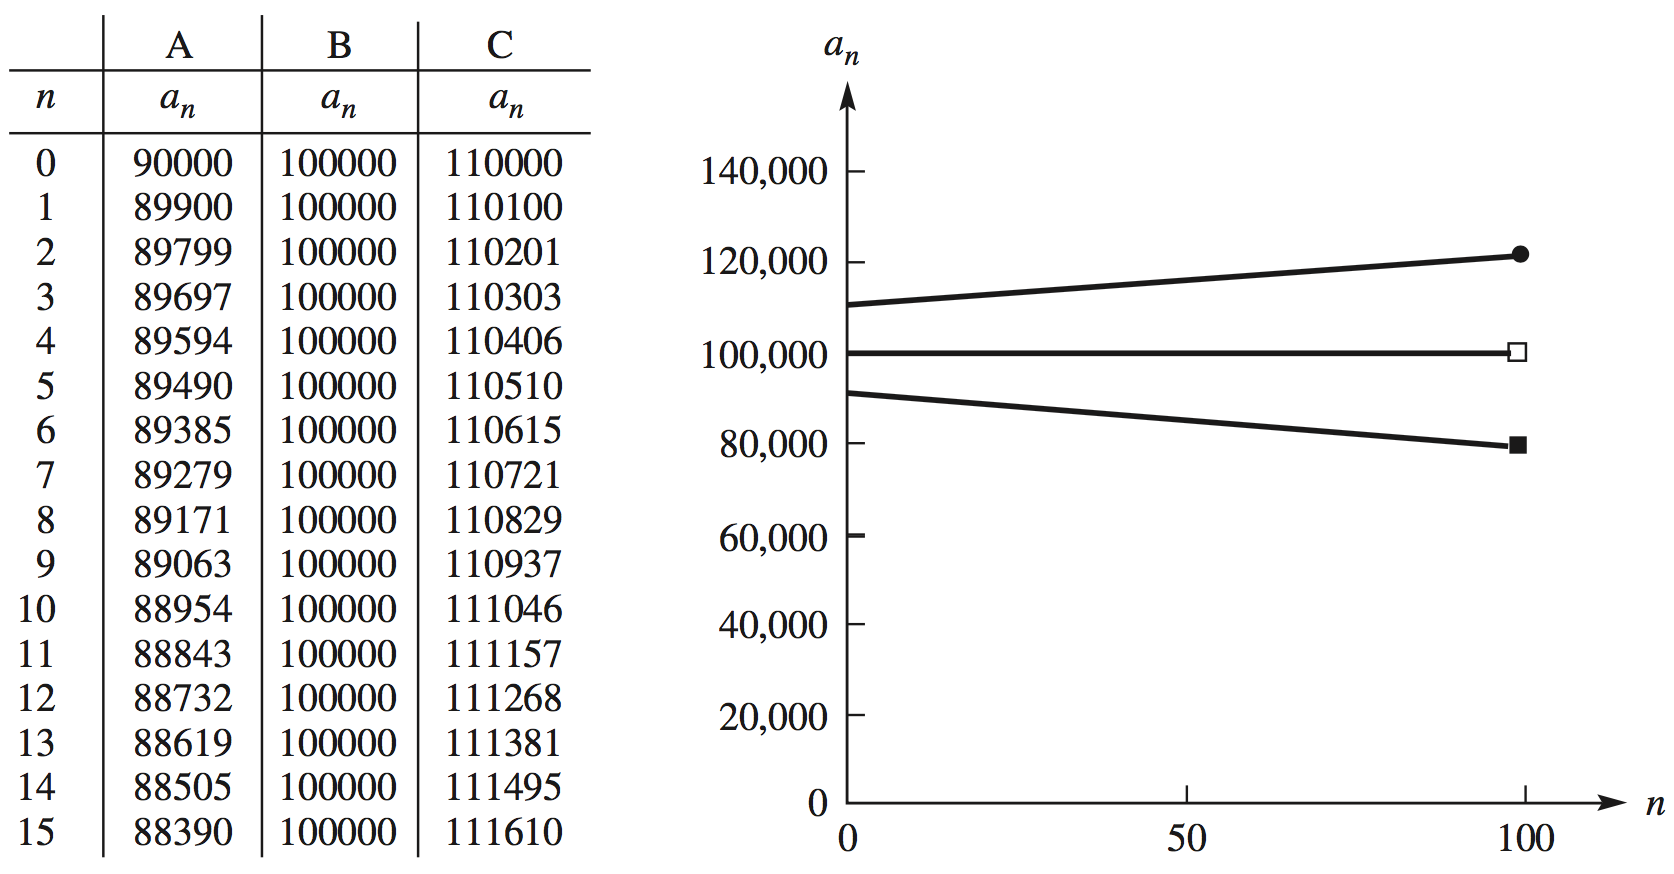
\includegraphics{invest.png}

}

\caption{投资}

\end{figure}%
\end{frame}

\begin{frame}{\(r = 1\)}
\phantomsection\label{r-1}
\[a_{n+1} = a_n -300\]

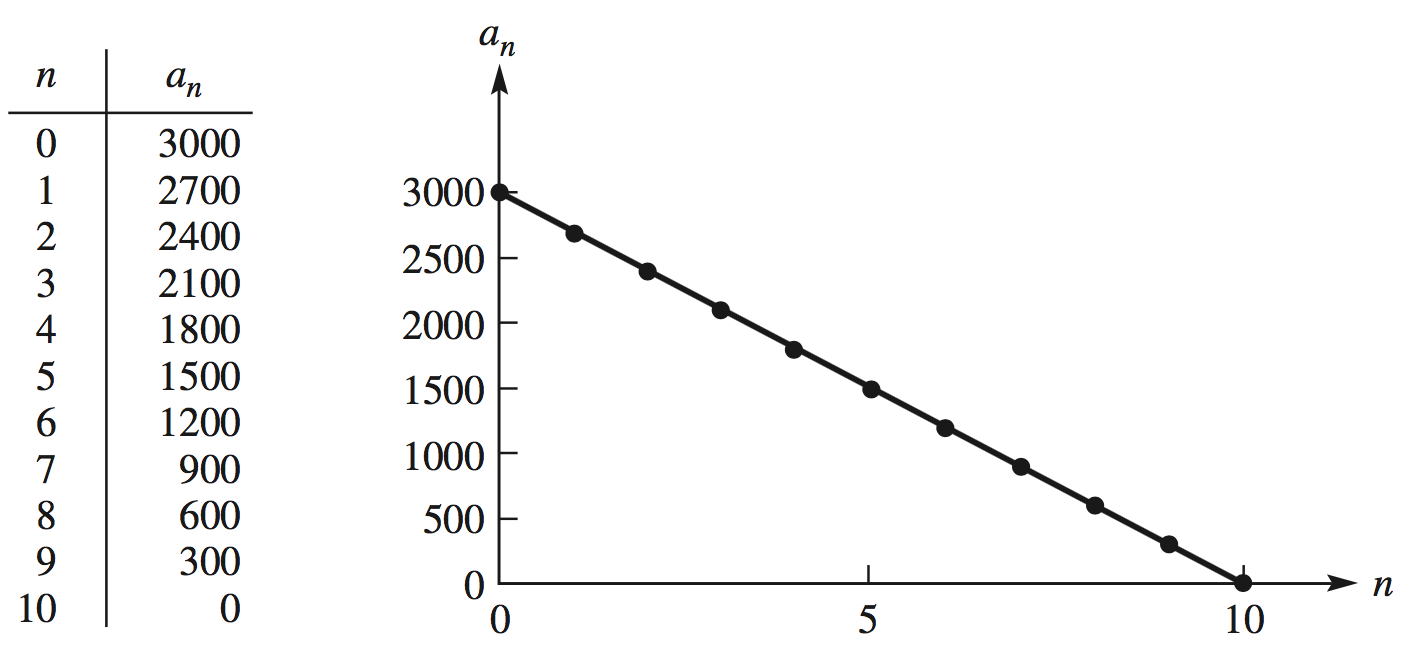
\includegraphics{poor.png}
\end{frame}

\begin{frame}{不动点}
\phantomsection\label{ux4e0dux52a8ux70b9-1}
\(a_{n+1} = ra_n + b, r \neq 1\)的不动点为:

\[a = \frac{b}{1-r}\]

上述动态系统的解为: \(a_k=r^kc+\frac{b}{1-r}\).

思考: \(r\)的值不同时,长期来说系统如何变化?
\end{frame}

\begin{frame}{非线性系统}
\phantomsection\label{ux975eux7ebfux6027ux7cfbux7edf}
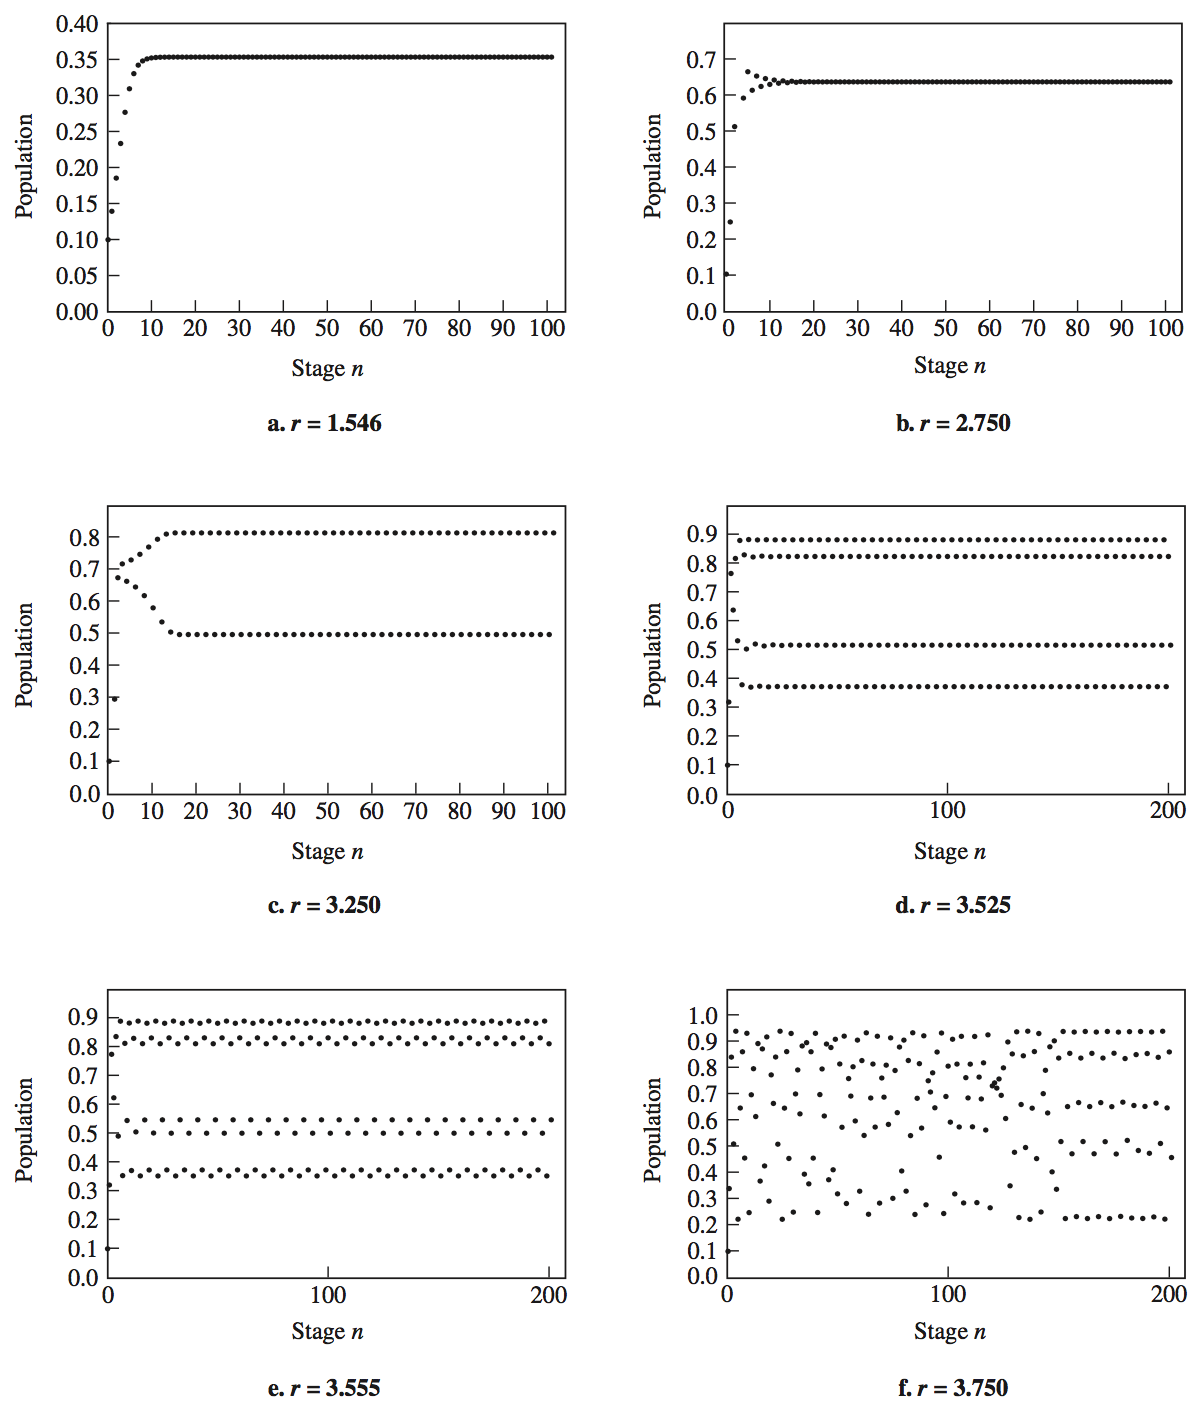
\includegraphics[width=0.4\textwidth,height=\textheight]{nonlinear.png}
\end{frame}

\begin{frame}{差分方程组}
\phantomsection\label{ux5deeux5206ux65b9ux7a0bux7ec4}
\begin{itemize}
\item
  找出不动点
\item
  当初始值在不动点附近时,系统如何变化
\end{itemize}

研究系统的长期变化,看系统对如下条件是否敏感:

\begin{itemize}
\item
  初始条件
\item
  对模型中的常量进行扰动
\end{itemize}
\end{frame}

\begin{frame}{汽车租赁公司}
\phantomsection\label{ux6c7dux8f66ux79dfux8d41ux516cux53f8}
\begin{columns}[T]
\begin{column}{0.8\textwidth}
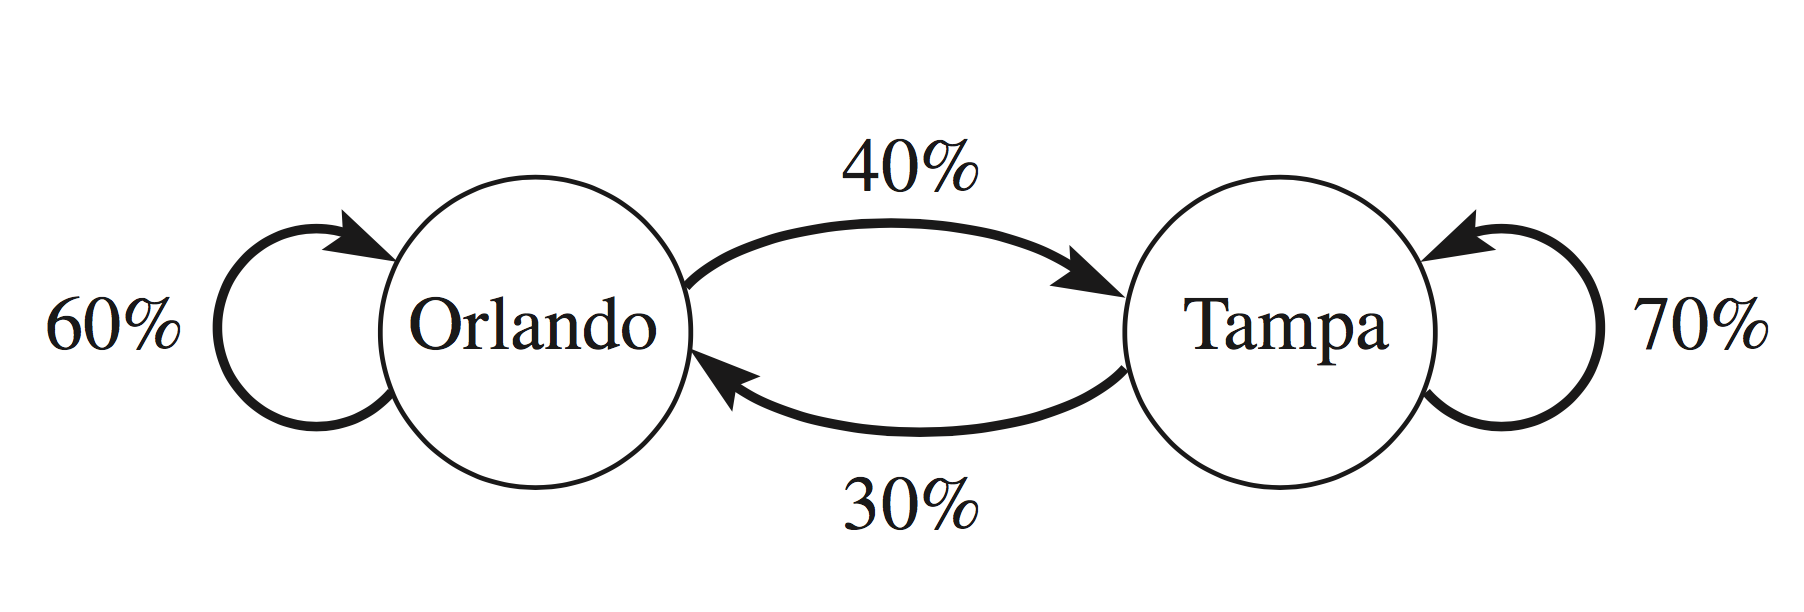
\includegraphics{taxi.png}
\end{column}
\end{columns}

\begin{description}
\tightlist
\item[\(O_n\)]
第\(n\)天营业结束时在奥兰多的车辆数
\item[\(T_n\)]
第\(n\)天营业结束时在坦帕的车辆数
\end{description}

\[
\begin{align*}
O_{n+1} &=0.6O_n + 0.3T_n \\
T_{n+1} &=0.4O_n + 0.7T_n
\end{align*}
\]
\end{frame}

\begin{frame}{计算平衡点}
\phantomsection\label{ux8ba1ux7b97ux5e73ux8861ux70b9}
如果存在平衡点\(O\), \(T\): \[O=O_{n+1}=O_n\] \[T=T_{n+1}=T_n\] 推导出:
\[O=0.6O + 0.3T\] \[T=0.4O + 0.7T\]
\end{frame}

\begin{frame}{方程求解}
\phantomsection\label{ux65b9ux7a0bux6c42ux89e3}
\(O=\frac{3}{4}T\)满足上述方程组.
如果公司有7000辆车,则\((O, T) = (3000, 4000)\)处开始,保持不变。

分析下述四种初始条件:

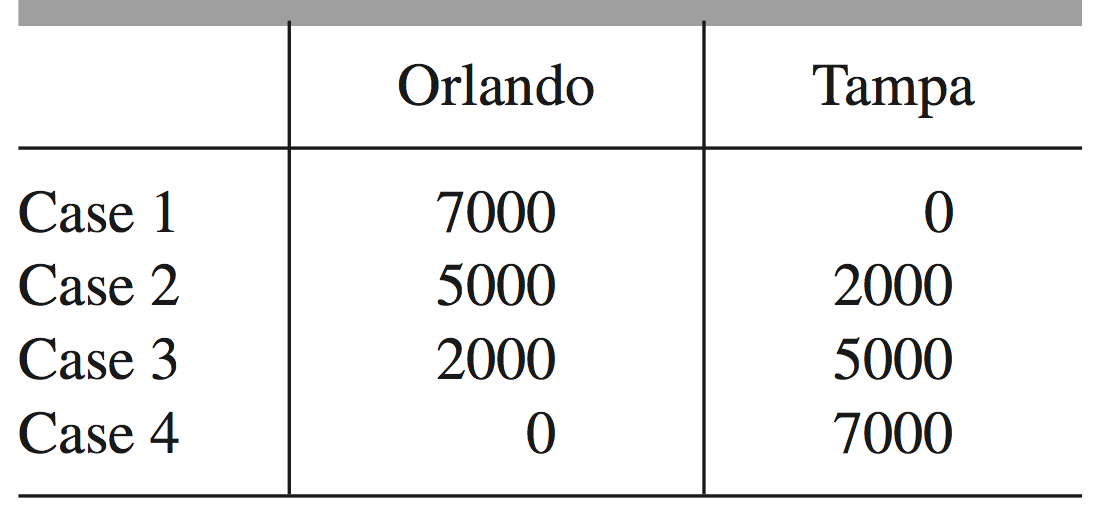
\includegraphics[width=0.4\textwidth,height=\textheight]{taxi-cases.png}
\end{frame}

\begin{frame}{分析}
\phantomsection\label{ux5206ux6790}
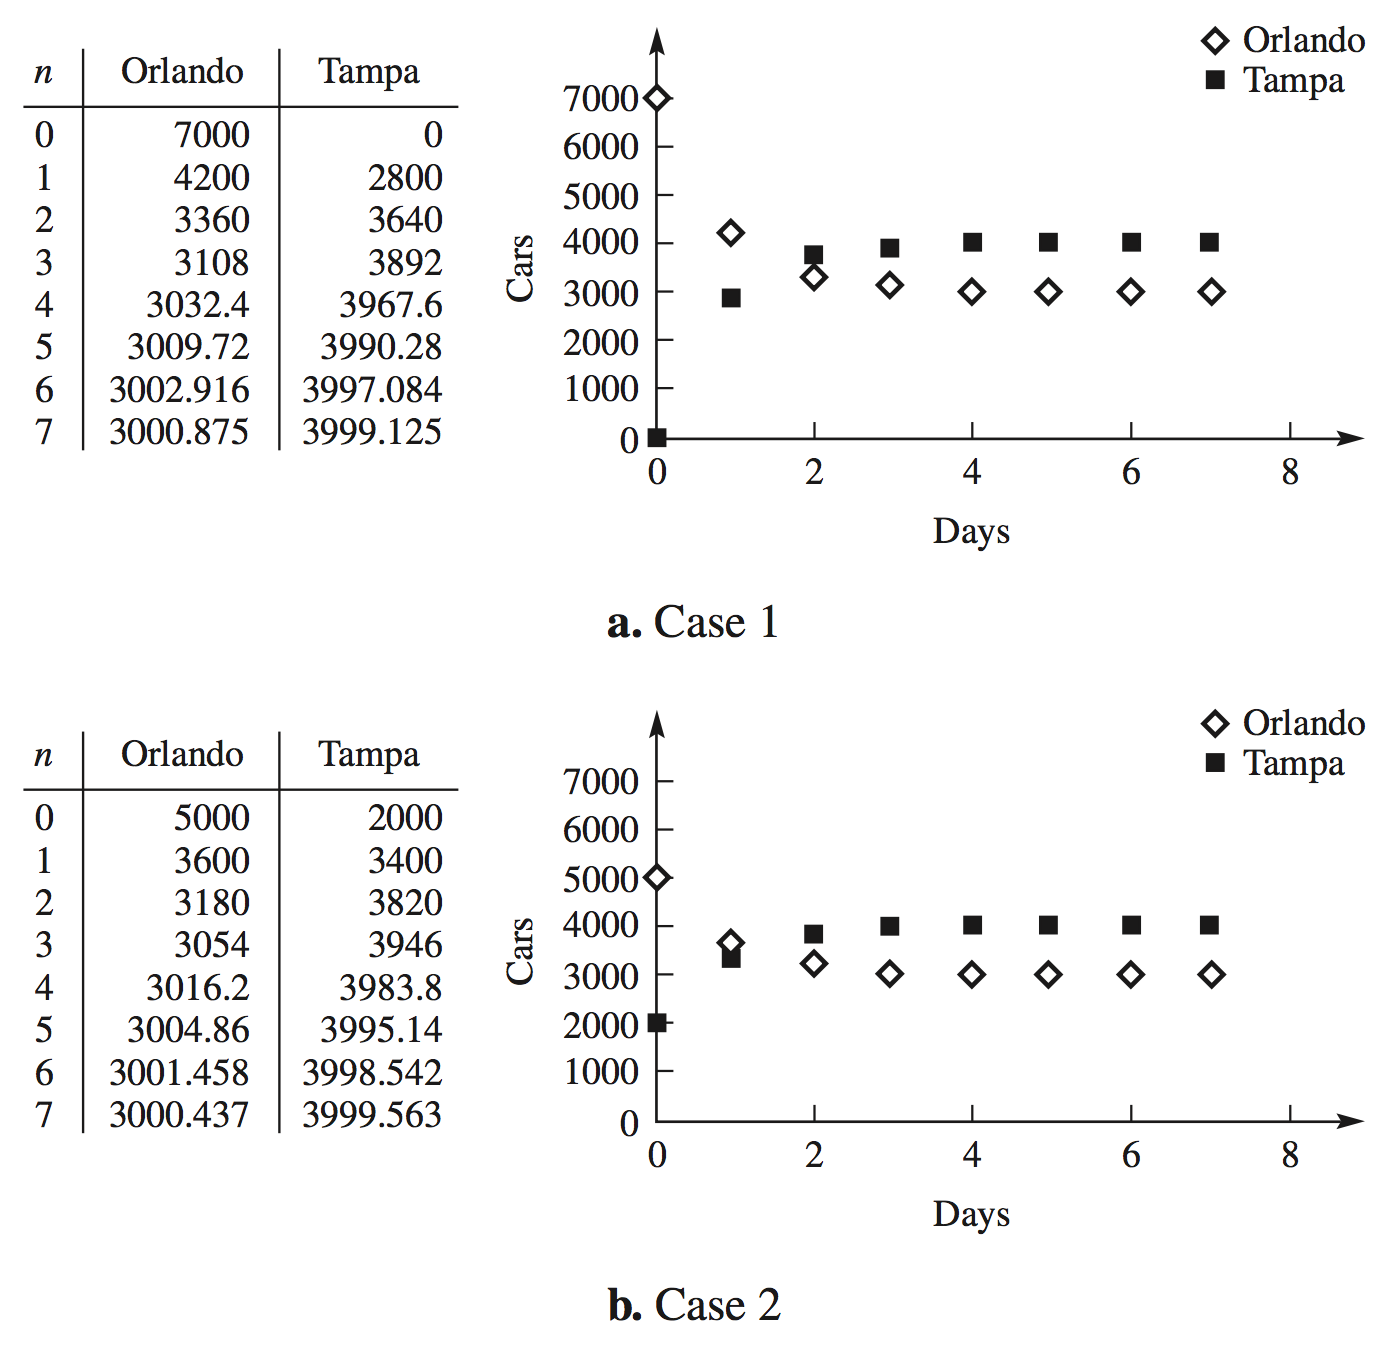
\includegraphics[width=0.4\textwidth,height=\textheight]{taxi-case12.png}
\end{frame}

\begin{frame}{分析}
\phantomsection\label{ux5206ux6790-1}
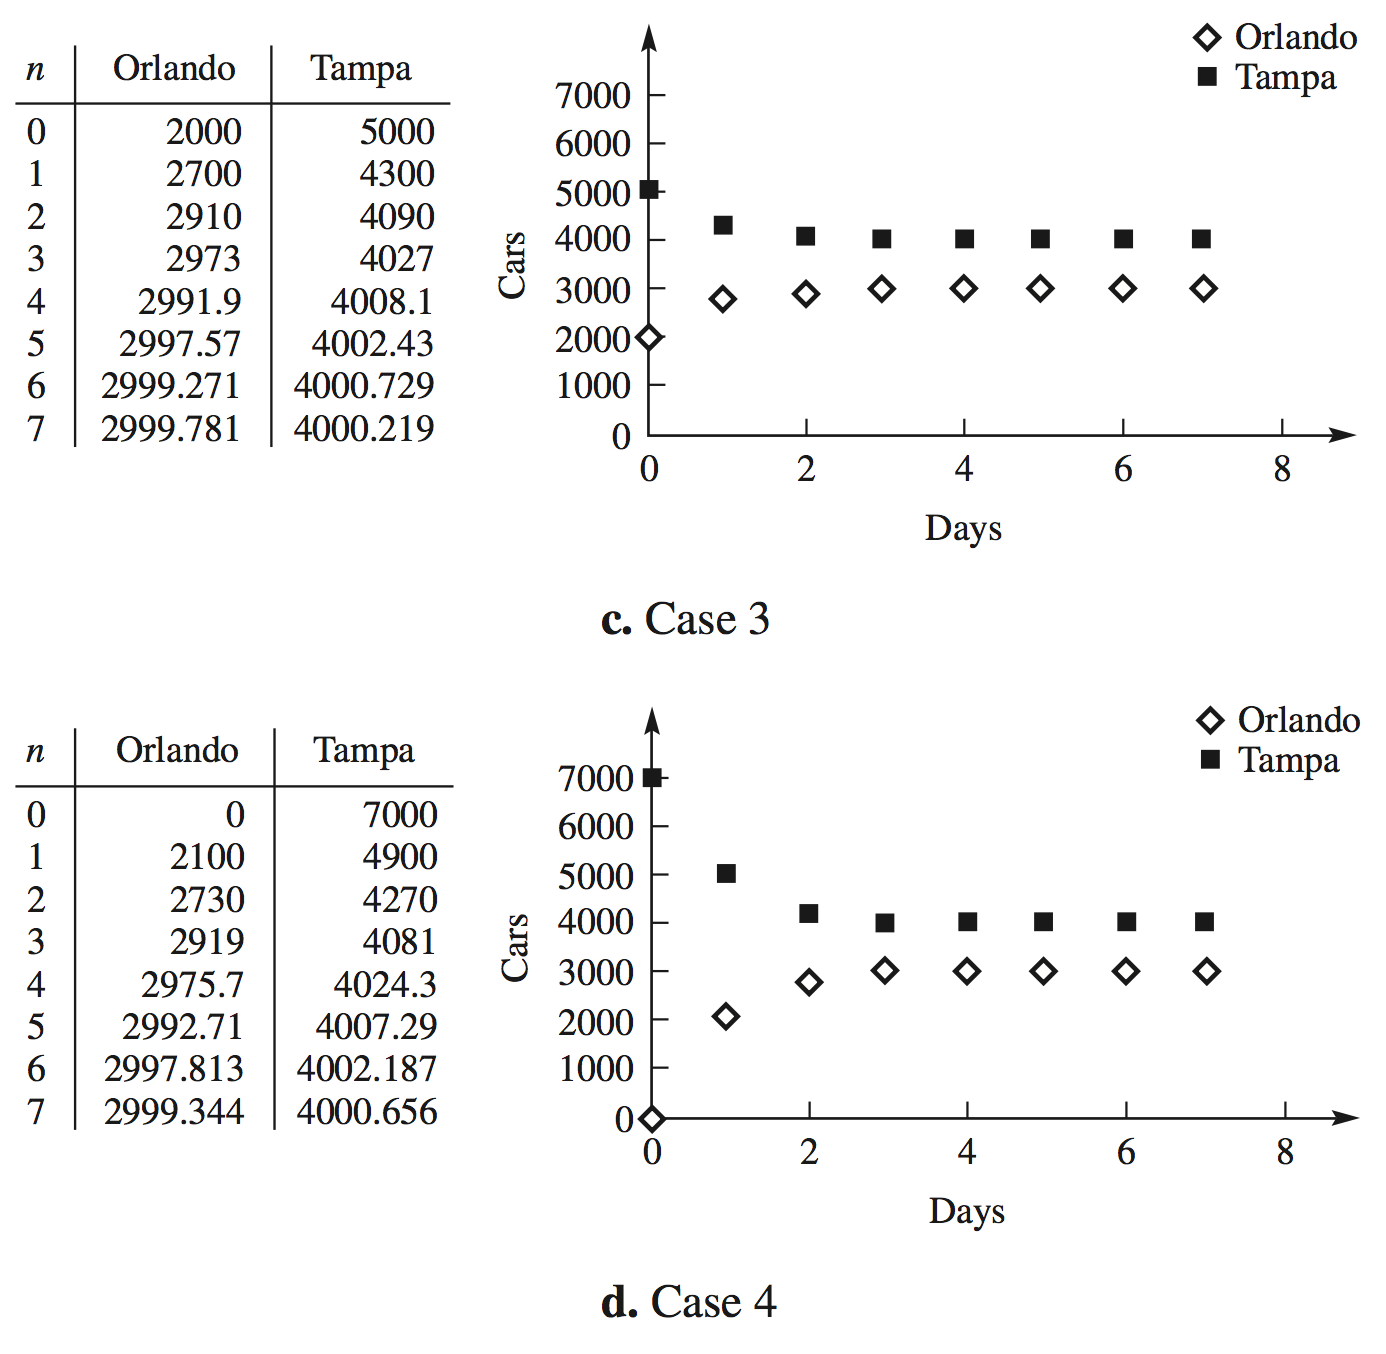
\includegraphics[width=0.4\textwidth,height=\textheight]{taxi-case34.png}
\end{frame}

\begin{frame}{结论}
\phantomsection\label{ux7ed3ux8bba}
四种情形中每一种情形在一周内都是和平衡点\((3000,4000)\)很接近的,甚至在其中一个城市没有车的情况也是如此。结果显示,平衡点是稳定的而且对初始值不敏感的。

思考:该系统是否对\(O_{n+1}\)和\(T_{n+1}\)的系数敏感?
\end{frame}

\begin{frame}{特拉法尔加战斗}
\phantomsection\label{ux7279ux62c9ux6cd5ux5c14ux52a0ux6218ux6597}
法西联军33艘战舰,英军27艘战舰,在一次遭遇战中每方的战舰损失都是对方战舰的\(10\%\)。

\textbf{动力系统模型} 令\(n\)表示战斗过程中遭遇战的阶段并定义:

\begin{itemize}
\tightlist
\item
  \(B_n =\)第\(n\)阶段英军的战舰数
\item
  \(F_n =\)第\(n\)阶段法西联军的战舰数
\end{itemize}
\end{frame}

\begin{frame}{死拼打法}
\phantomsection\label{ux6b7bux62fcux6253ux6cd5}
战斗结束:英军全面战败,剩3艘战舰其中一艘严重损坏,法军大约还有18艘战舰。

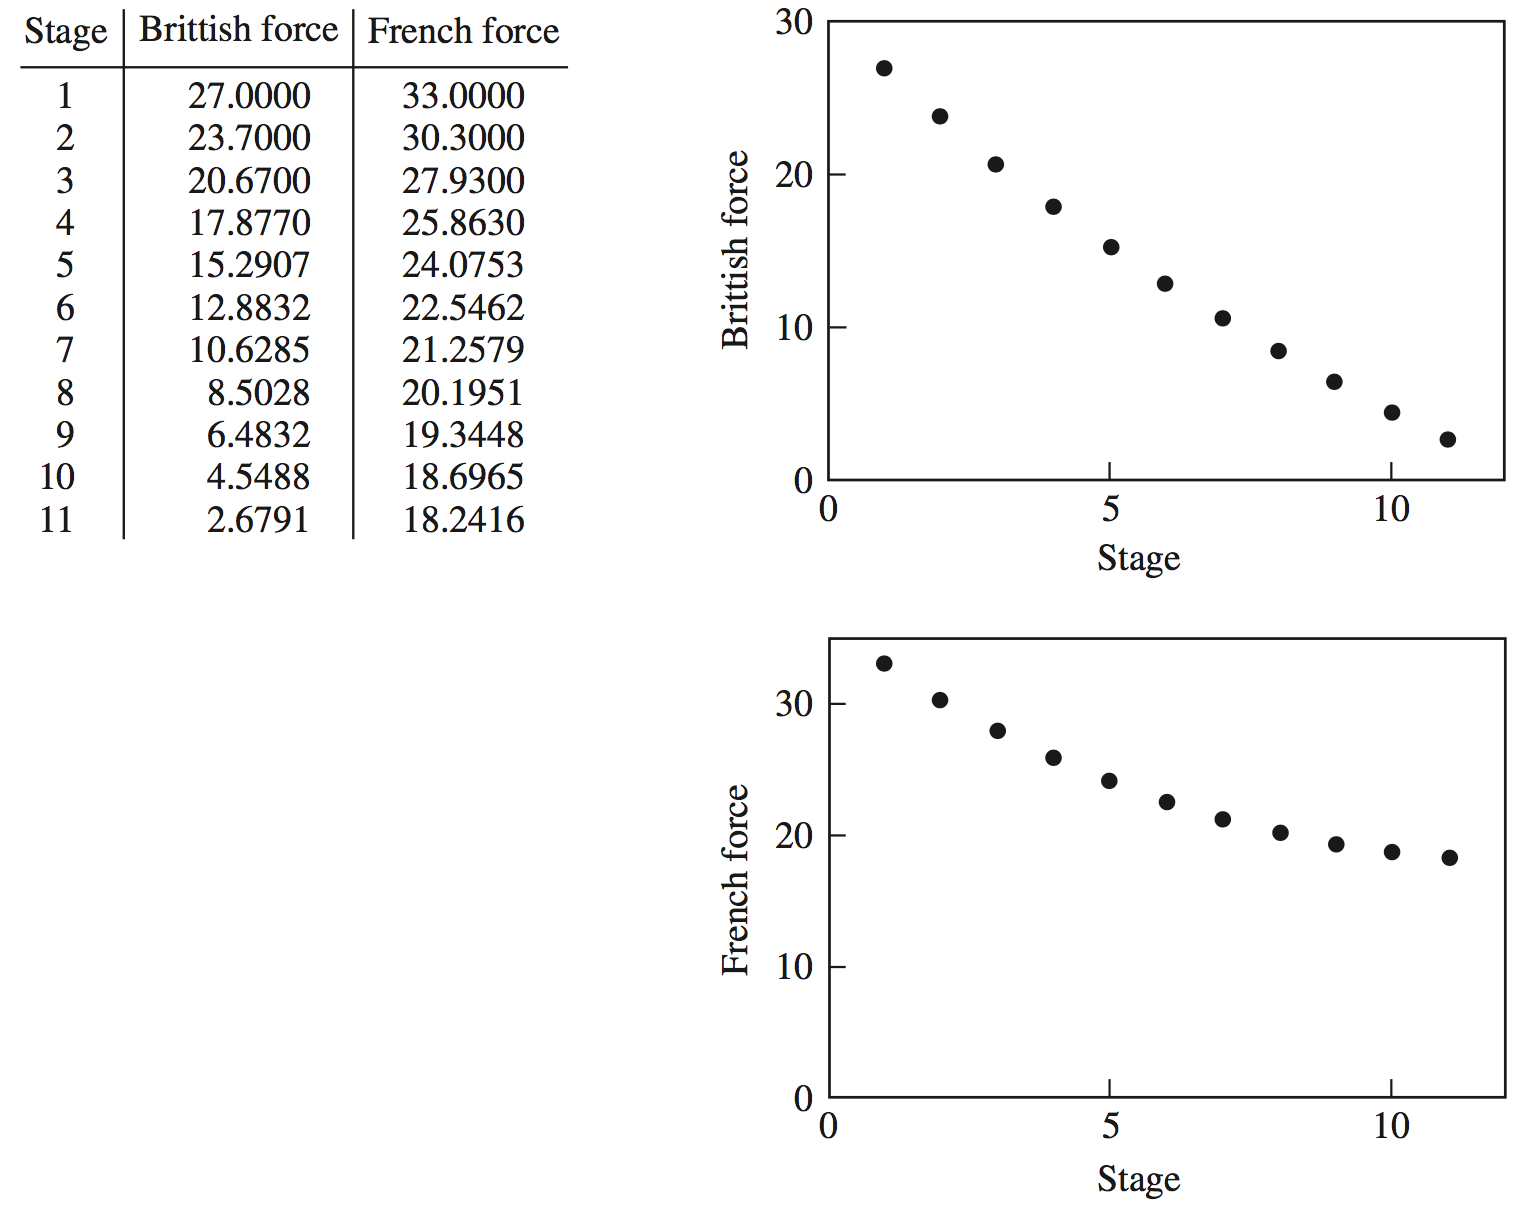
\includegraphics[width=0.4\textwidth,height=\textheight]{fight-death.png}
\end{frame}

\begin{frame}{各个击破}
\phantomsection\label{ux5404ux4e2aux51fbux7834}
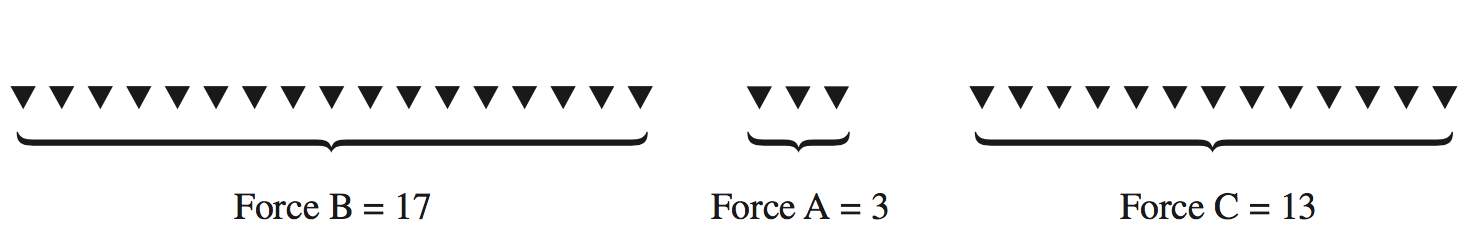
\includegraphics[width=0.4\textwidth,height=\textheight]{fight-france.png}

策略:英军13艘攻击\(A\);然后,全力攻击\(B\),最后攻击\(C\)。
\end{frame}

\begin{frame}{战斗A}
\phantomsection\label{ux6218ux6597a}
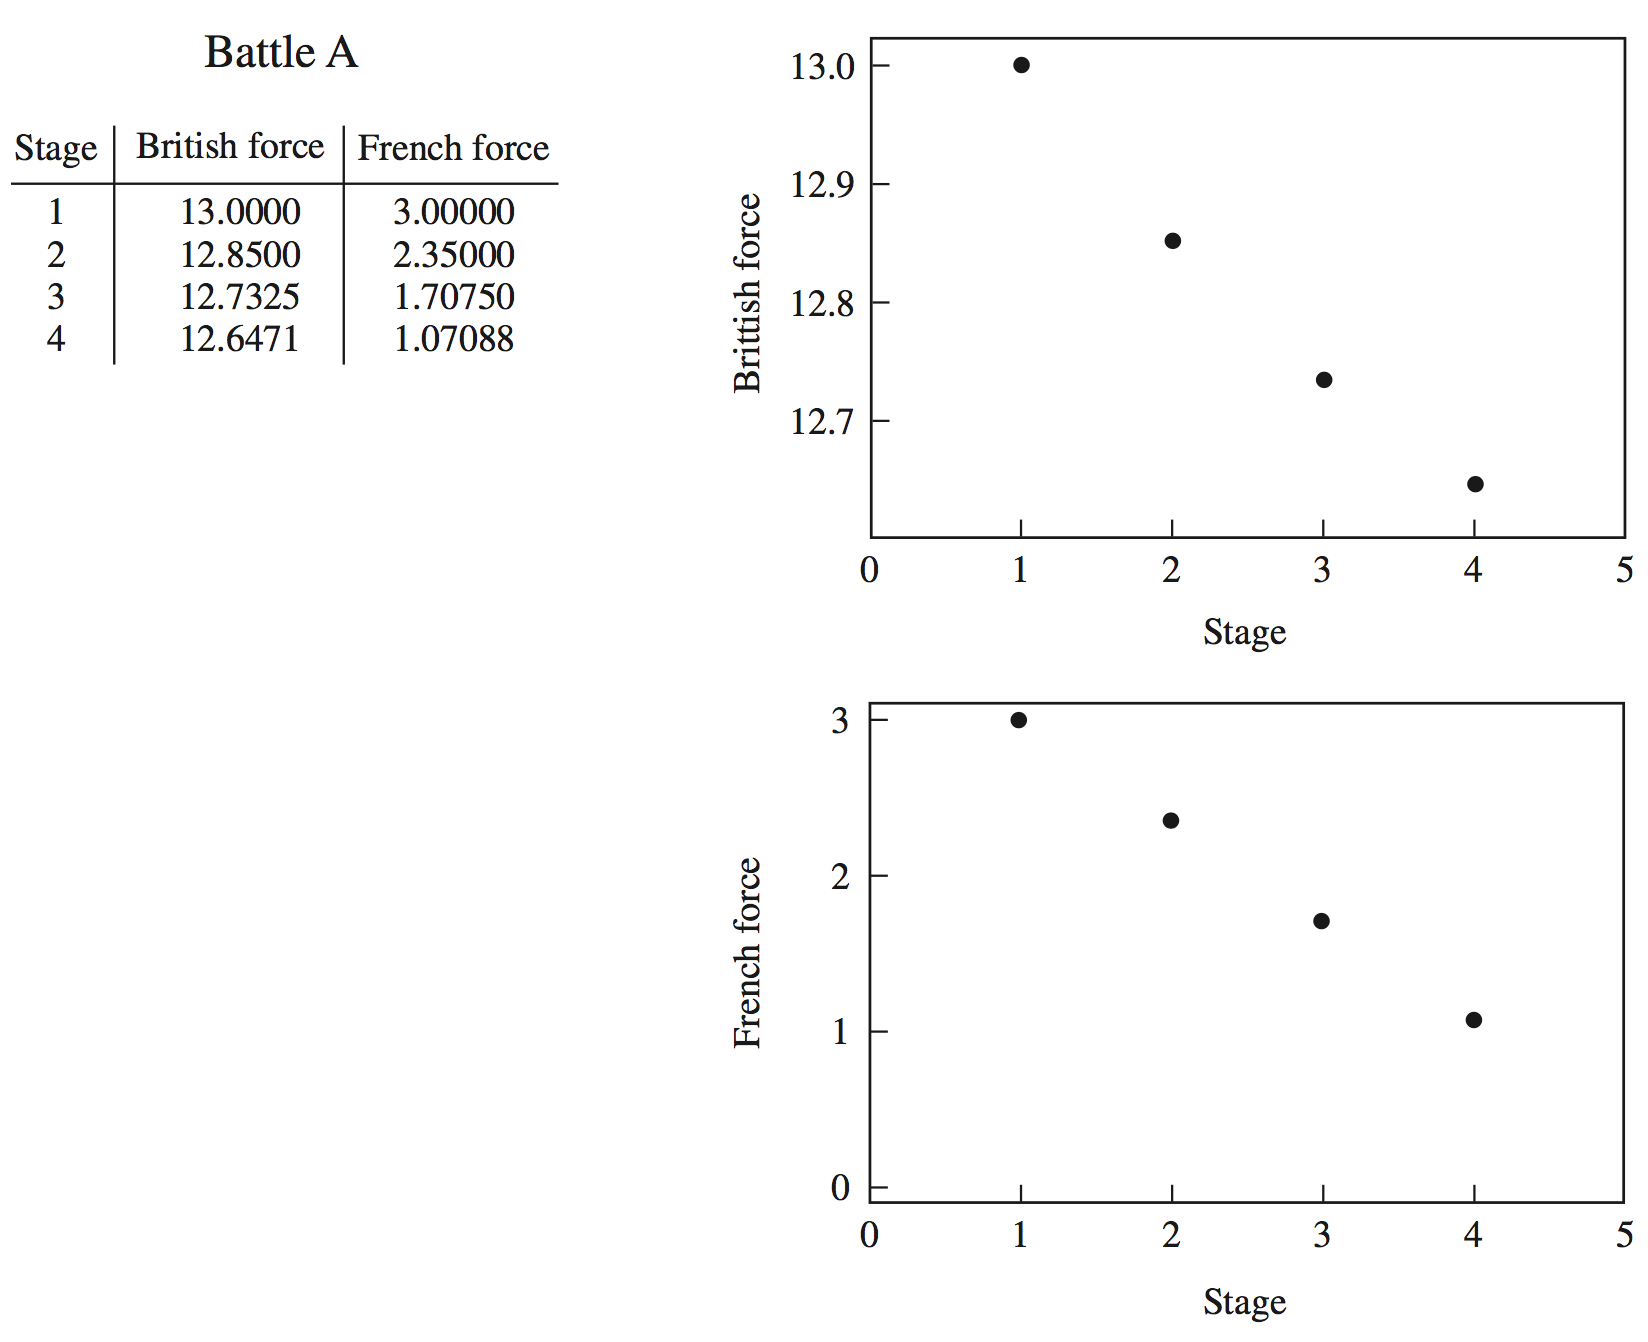
\includegraphics[width=0.4\textwidth,height=\textheight]{fight-A.png}
\end{frame}

\begin{frame}{战斗B}
\phantomsection\label{ux6218ux6597b}
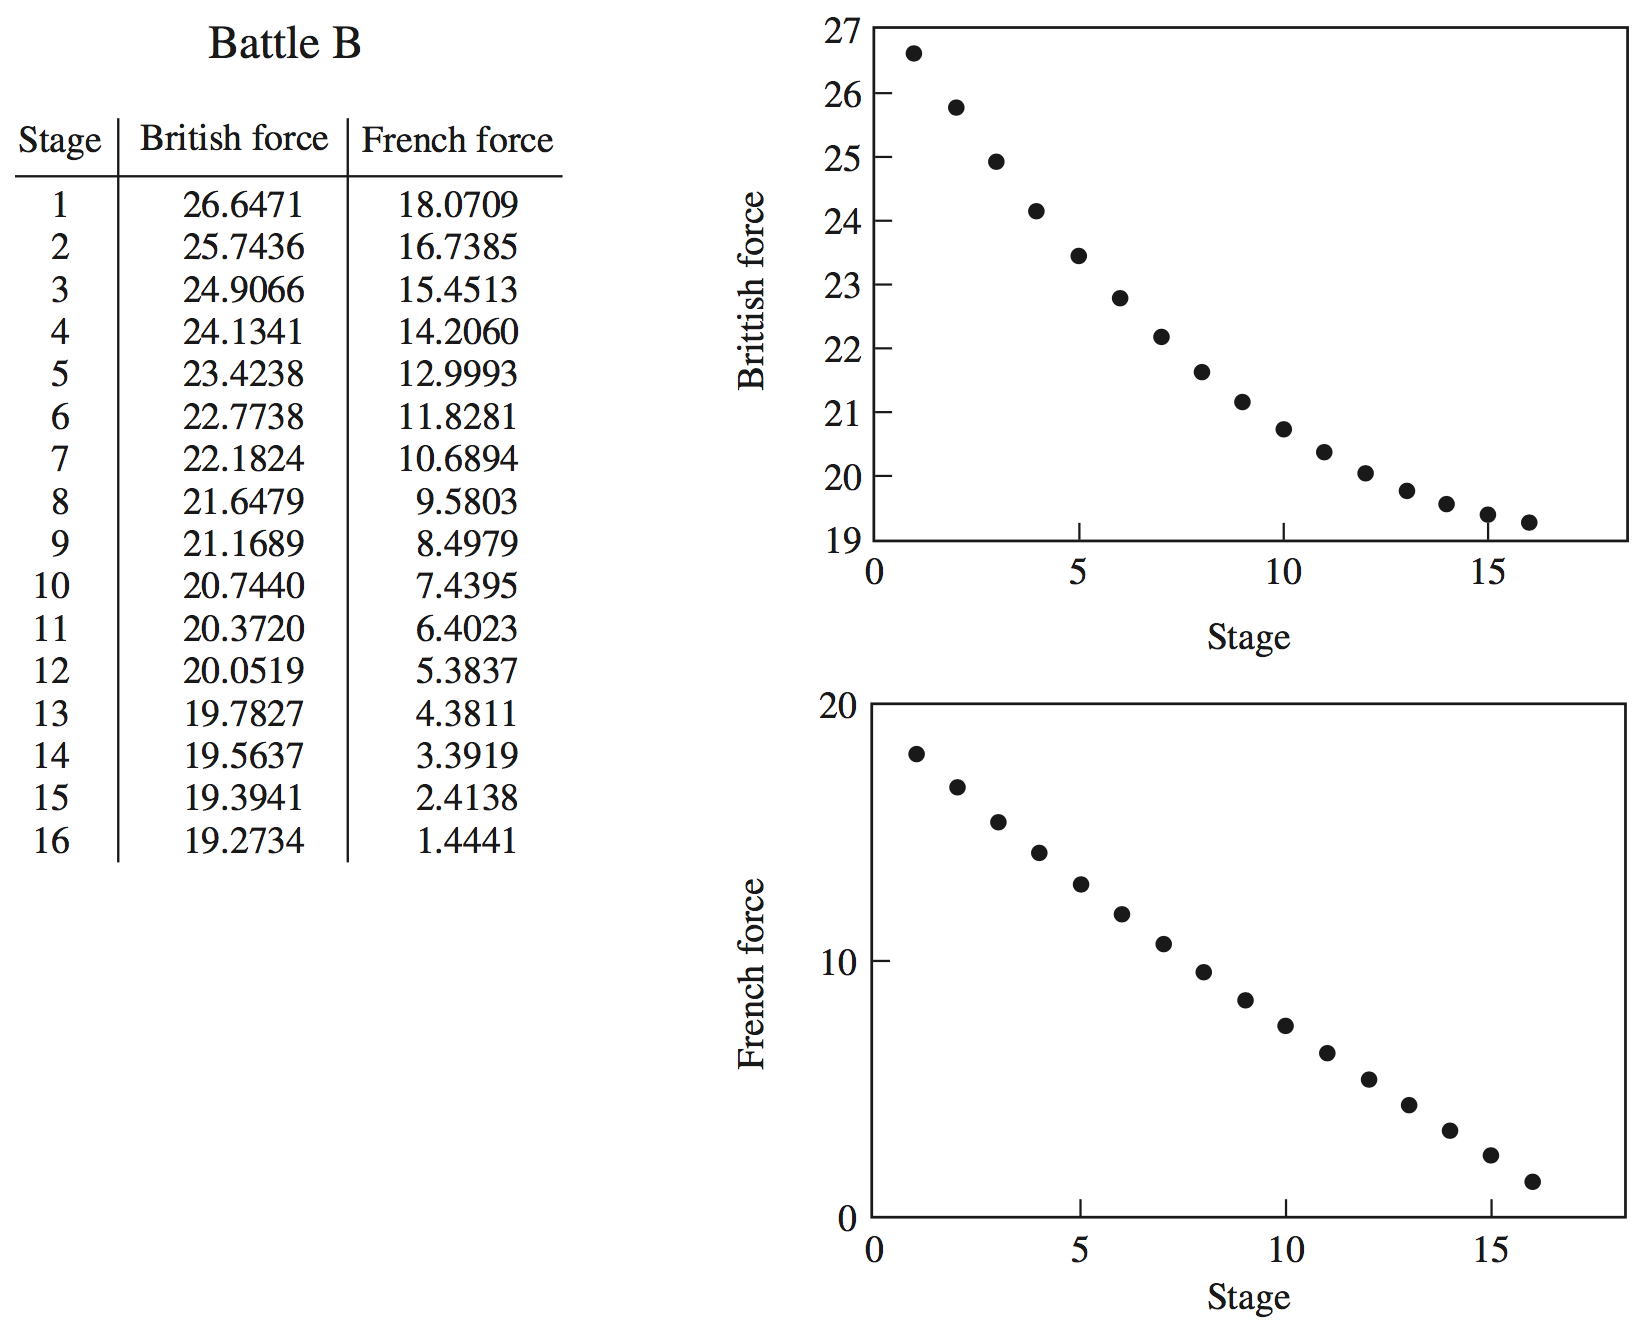
\includegraphics[width=0.4\textwidth,height=\textheight]{fight-B.png}
\end{frame}

\begin{frame}{战斗C}
\phantomsection\label{ux6218ux6597c}
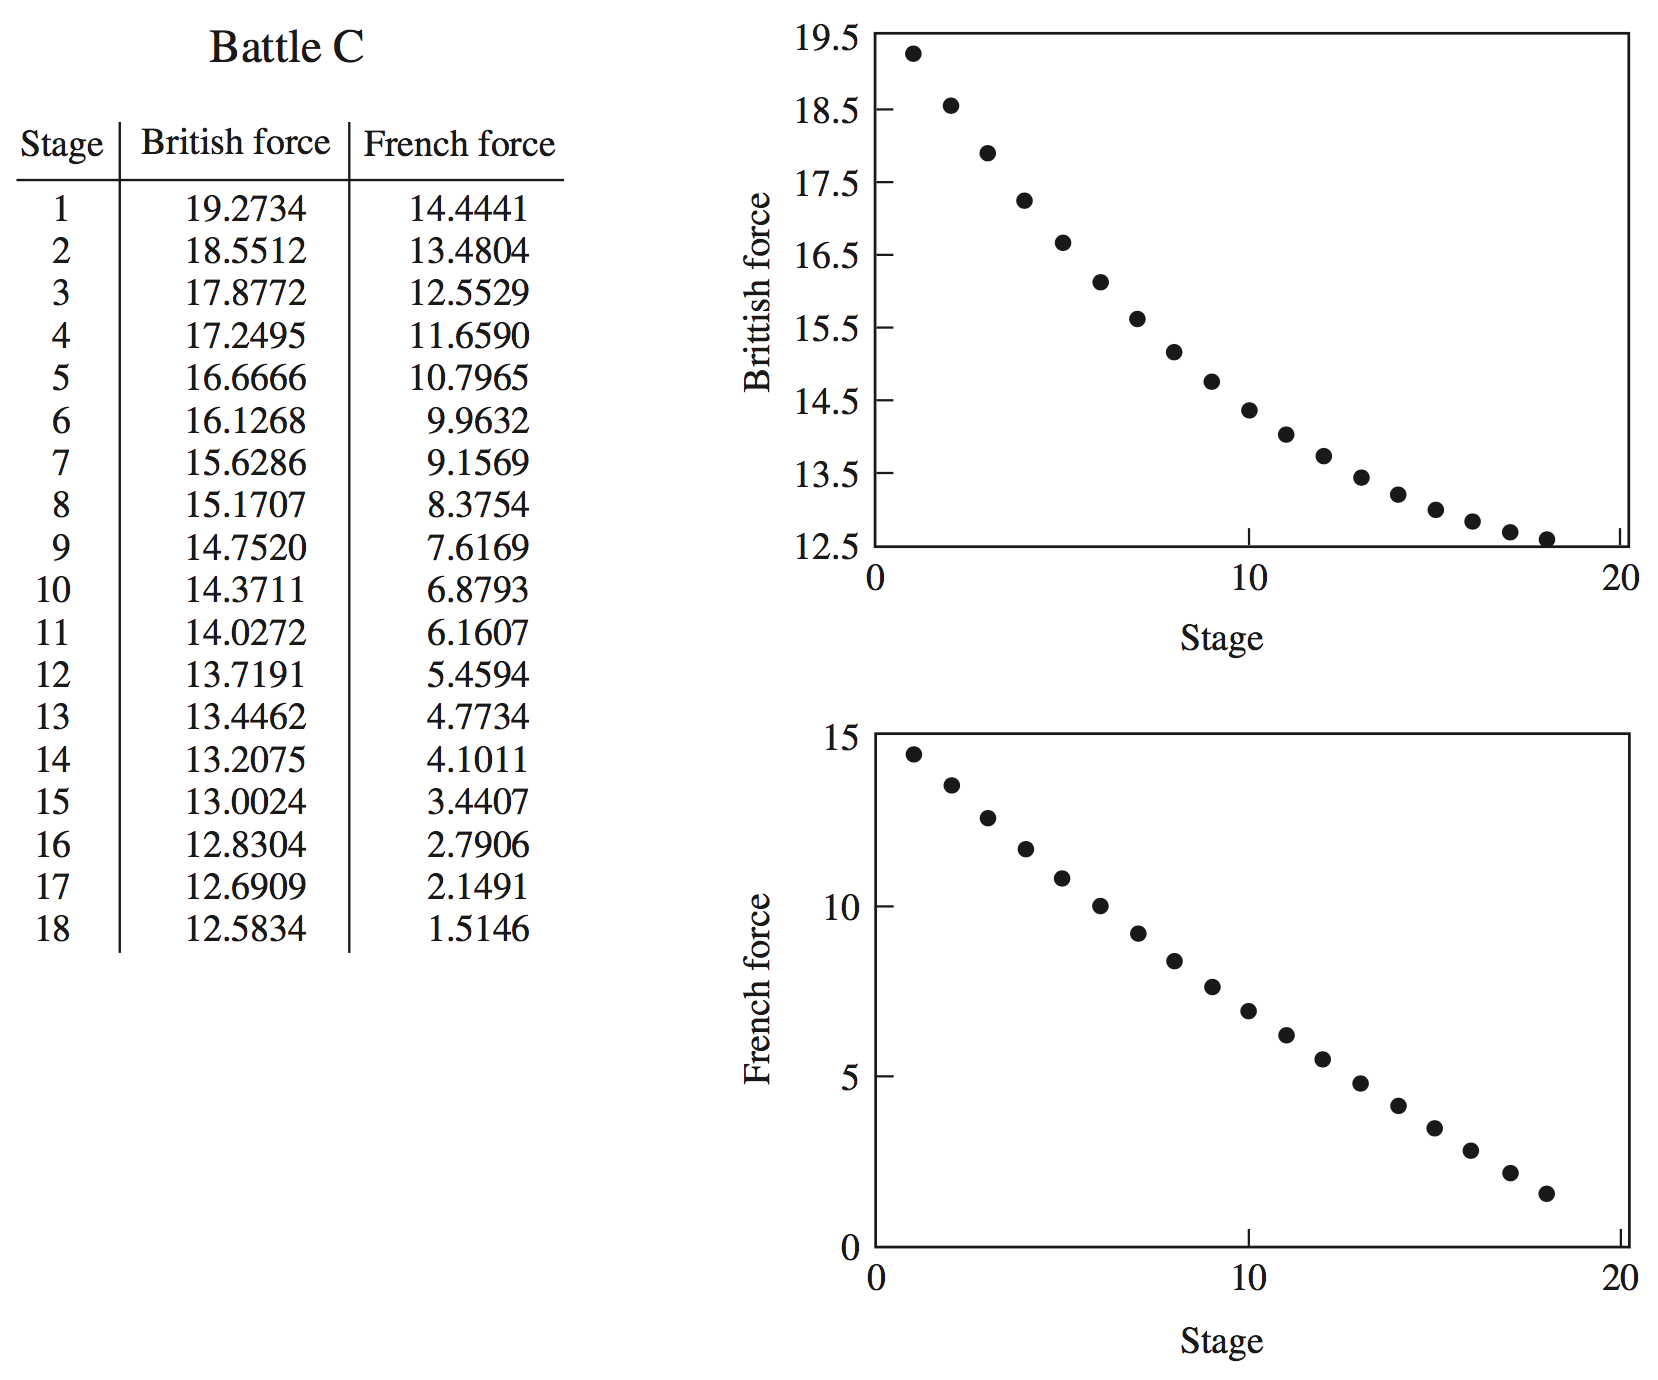
\includegraphics[width=0.4\textwidth,height=\textheight]{fight-C.png}
\end{frame}

\begin{frame}{战果}
\phantomsection\label{ux6218ux679c}
英军大获全胜。现实世界:法西联军没有参加战斗C,而是把剩下的约13艘战舰撤回法国。
\end{frame}

\begin{frame}{斑点猫头鹰和隼}
\phantomsection\label{ux6591ux70b9ux732bux5934ux9e70ux548cux96bc}
\begin{itemize}
\tightlist
\item
  \(O_n\), \(H_n\)分别表示第\(n\)天猫头鹰和隼的数量
\item
  \(\Delta O_n=k_1O_n\), \(\Delta H_n=k_2H_n\) (不考虑竞争)
\item
  \(\Delta O_n=k_1O_n - k_3O_nH_n\), \(\Delta H_n=k_2H_n-k_4O_nH_n\)
  (考虑竞争)
\item
  \(O_{n+1}=(1+k_1)O_n - k_3O_nH_n\)
\item
  \(H_{n+1}=(1+k_2)H_n-k_4O_nH_n\)
\end{itemize}
\end{frame}

\begin{frame}{求解平衡点}
\phantomsection\label{ux6c42ux89e3ux5e73ux8861ux70b9}
\begin{itemize}
\tightlist
\item
  \(O_{n+1}=1.2O_n - 0.001O_nH_n\)
\item
  \(H_{n+1}=1.3H_n - 0.002O_nH_n\)
\end{itemize}

如果\((O,H)\)为平衡点则\(O_{n+1}=O_n=O\), \(H_{n+1}=H_n=H\):

\begin{itemize}
\tightlist
\item
  \(O=1.2O - 0.001OH \Rightarrow O = 0 or H = 200\)
\item
  \(H=1.3H - 0.002OH \Rightarrow H = 0 or O = 150\)
\end{itemize}
\end{frame}

\begin{frame}{平衡点分析}
\phantomsection\label{ux5e73ux8861ux70b9ux5206ux6790}
两个平衡点: \((0, 0)\), \((150, 200)\). 为什么?

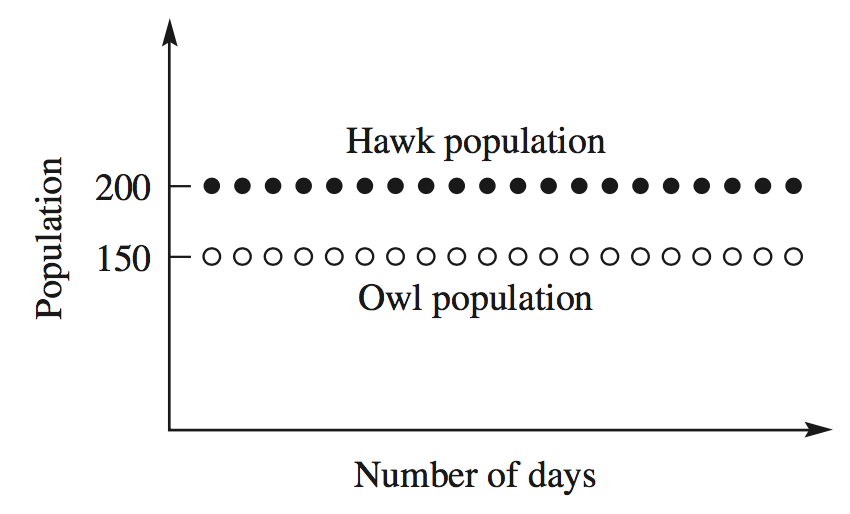
\includegraphics[width=0.4\textwidth,height=\textheight]{owl.png}
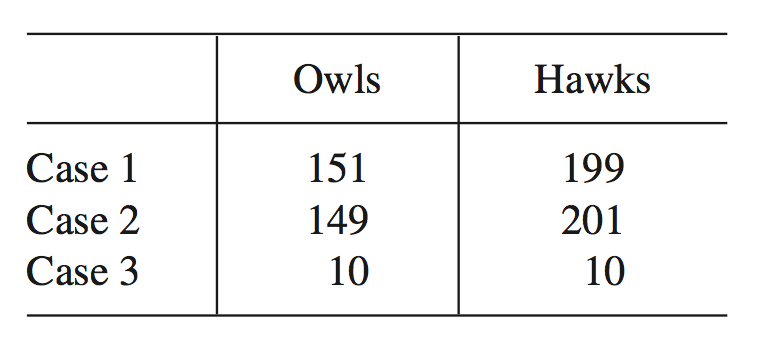
\includegraphics[width=0.4\textwidth,height=\textheight]{owl-start.png}
\end{frame}

\begin{frame}{情况1}
\phantomsection\label{ux60c5ux51b51}
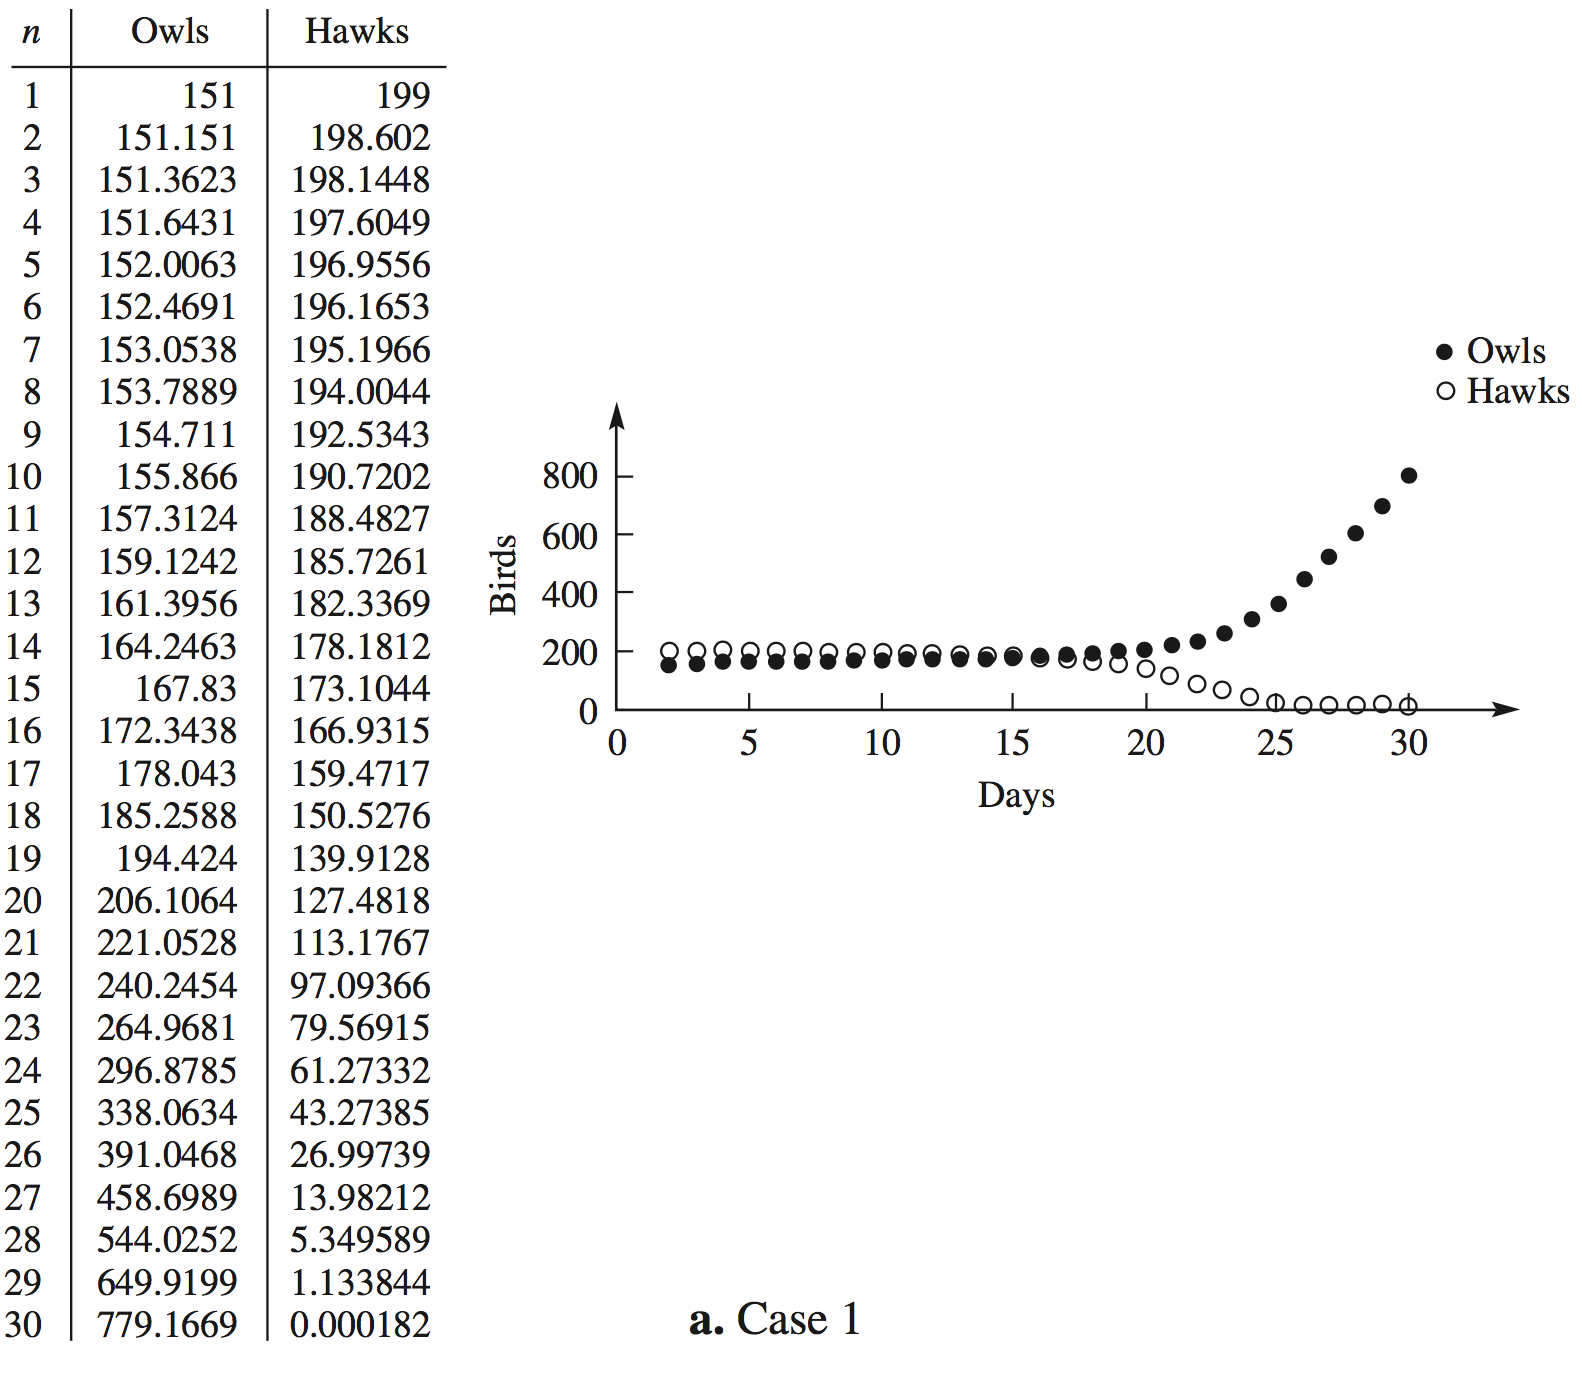
\includegraphics[width=0.4\textwidth,height=\textheight]{owl-1.png}
\end{frame}

\begin{frame}{情况2}
\phantomsection\label{ux60c5ux51b52}
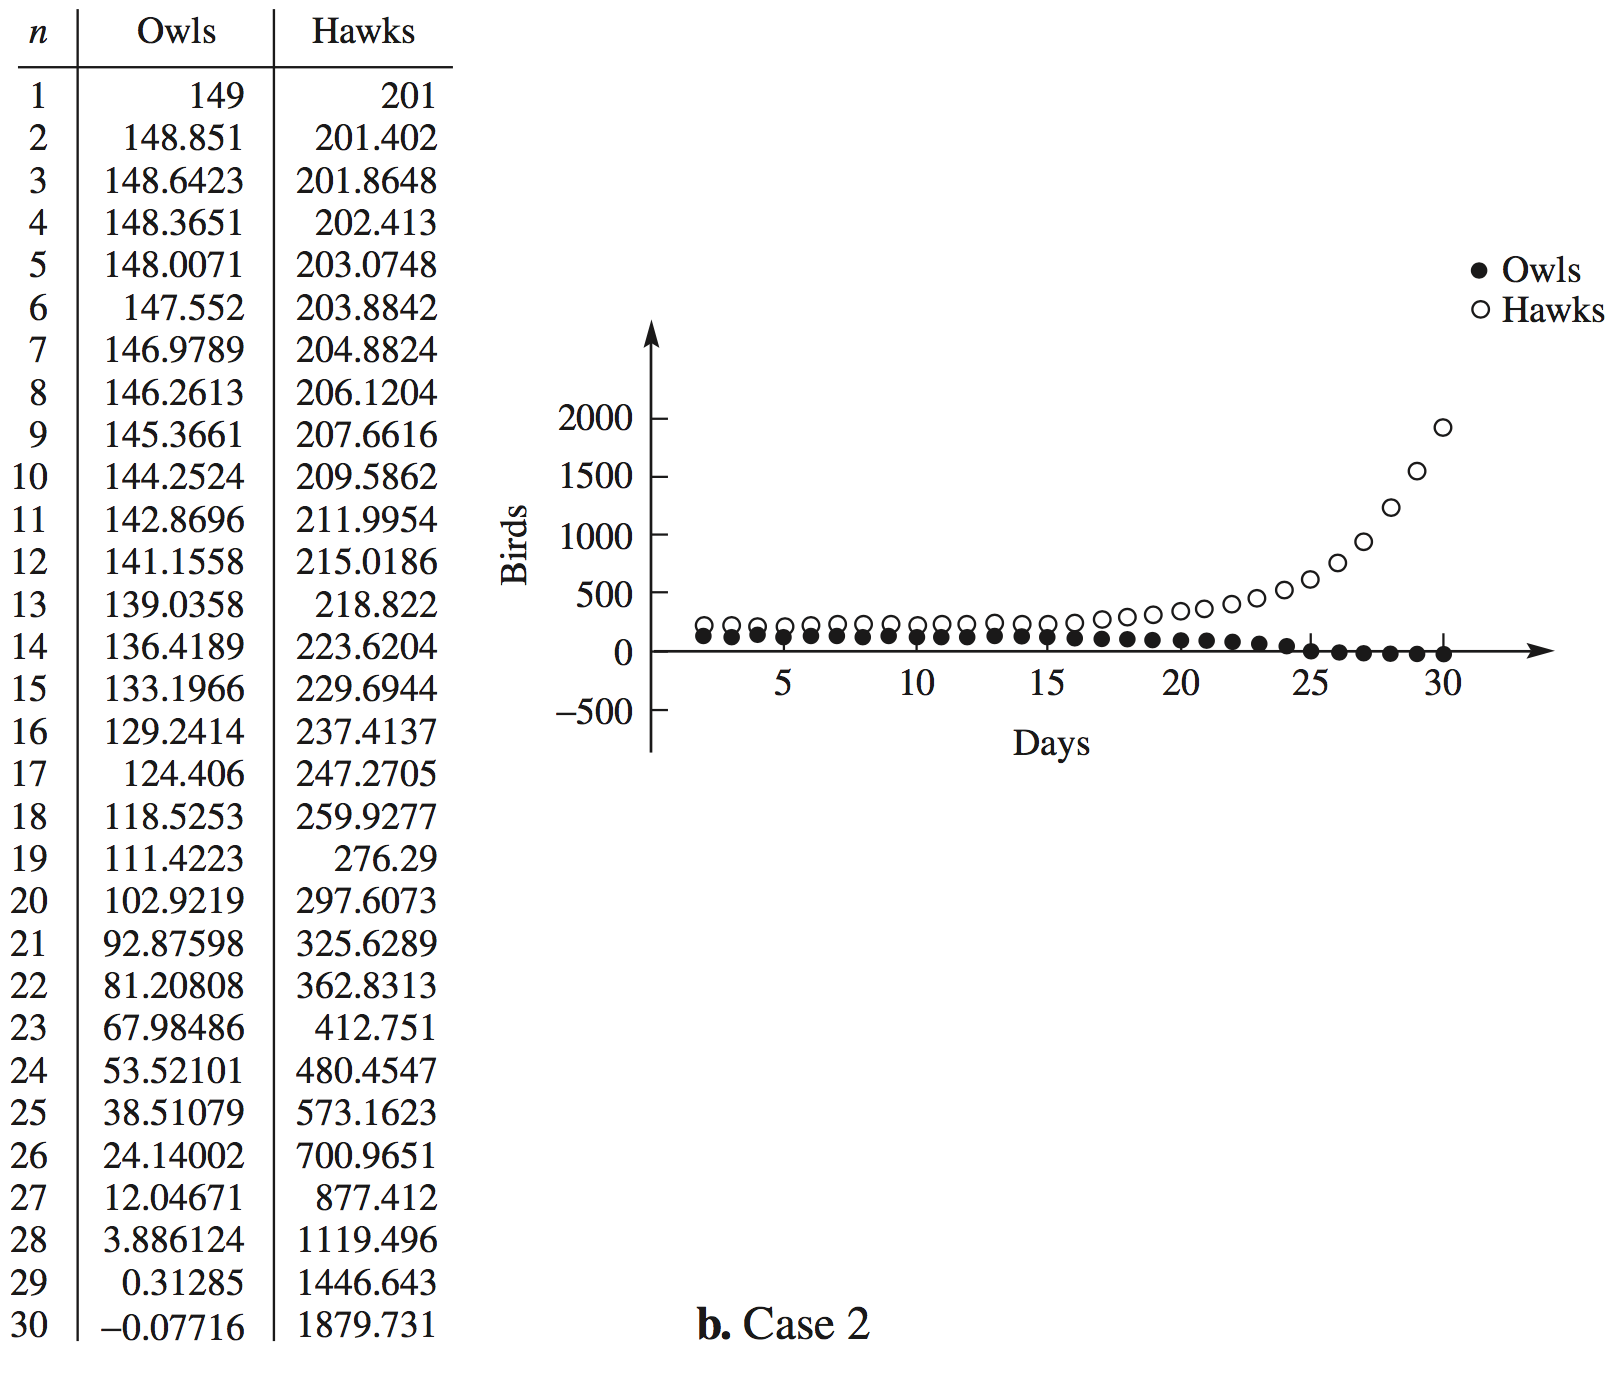
\includegraphics[width=0.4\textwidth,height=\textheight]{owl-2.png}
\end{frame}

\begin{frame}{情况3}
\phantomsection\label{ux60c5ux51b53}
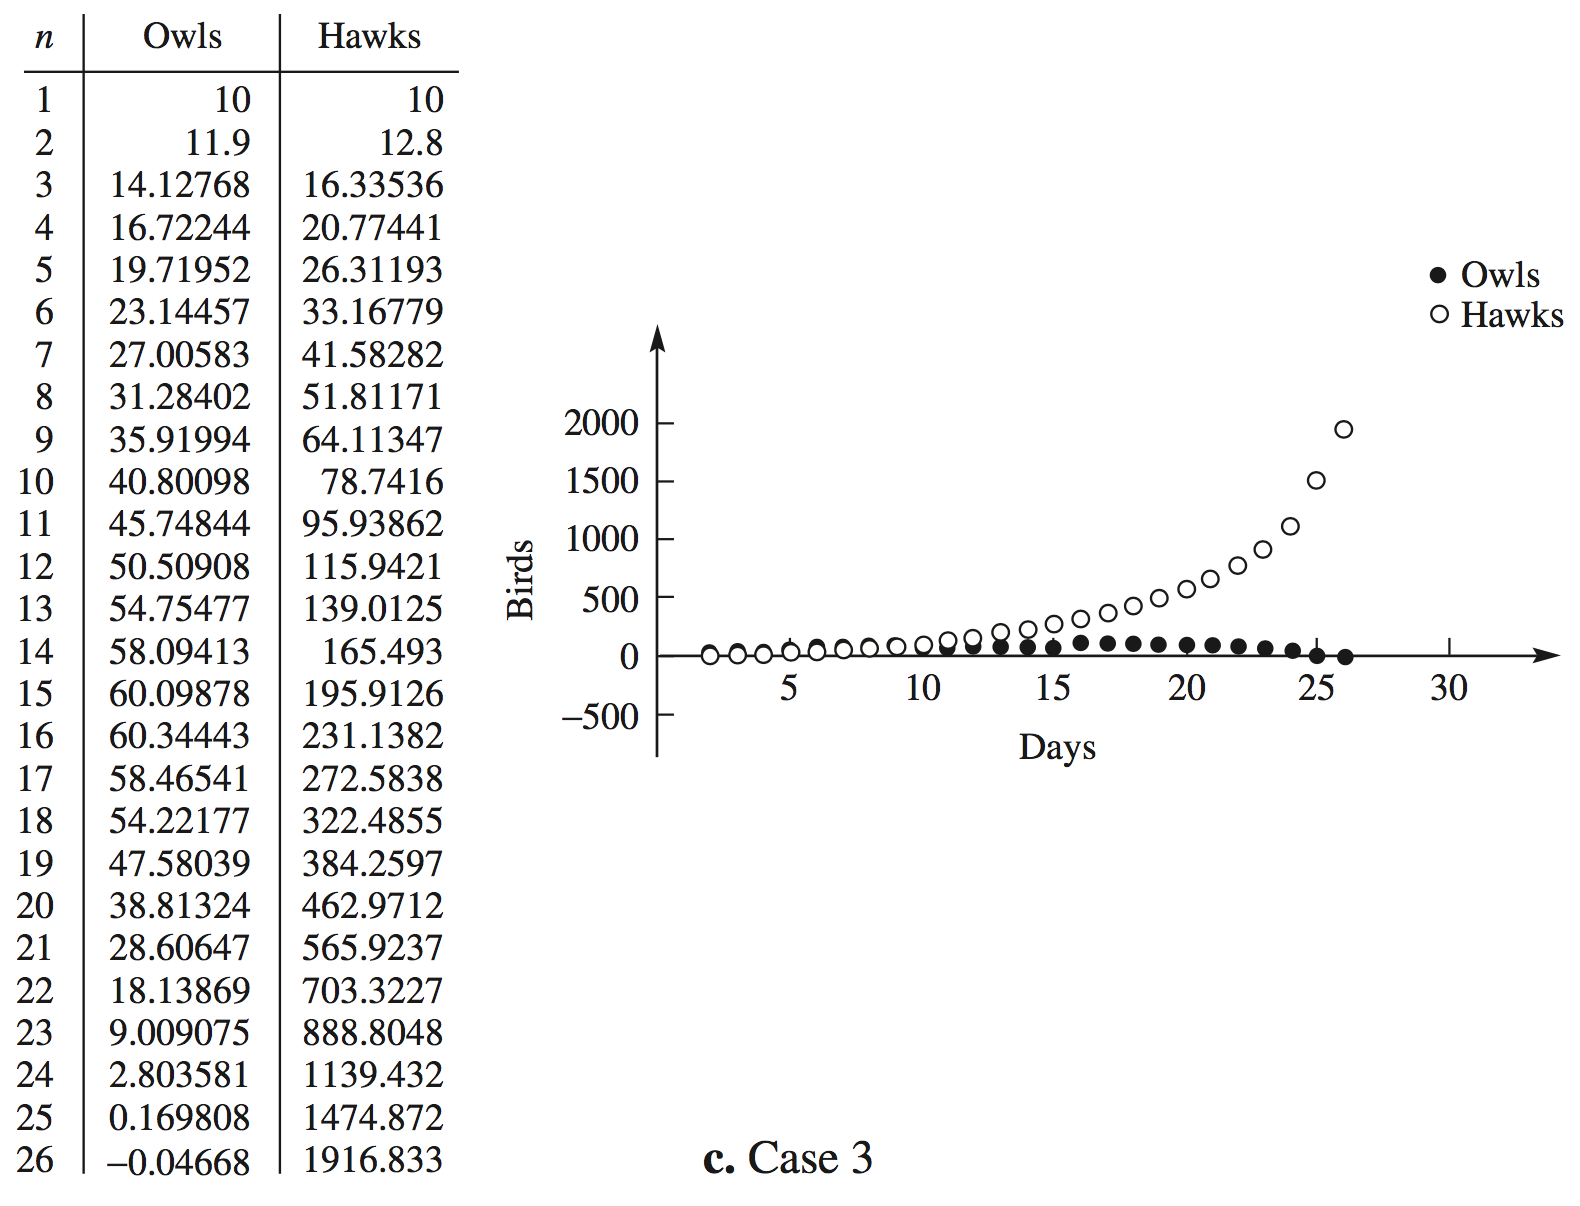
\includegraphics[width=0.4\textwidth,height=\textheight]{owl-3.png}
\end{frame}

\begin{frame}{对初始条件的敏感性和长期行为}
\phantomsection\label{ux5bf9ux521dux59cbux6761ux4ef6ux7684ux654fux611fux6027ux548cux957fux671fux884cux4e3a}
如果在栖息地安置350只猫头鹰和隼:

\begin{enumerate}
\tightlist
\item
  如果150头为猫头鹰:猫头鹰和隼的数量不变(150、200)
\item
  如果149头或更少猫头鹰:猫头鹰将灭绝
\item
  如果151头或更多猫头鹰:隼将灭绝
\item
  该模型对初始条件极其敏感,平衡点不稳定。
\end{enumerate}
\end{frame}

\begin{frame}{旅客趋势}
\phantomsection\label{ux65c5ux5ba2ux8d8bux52bf}
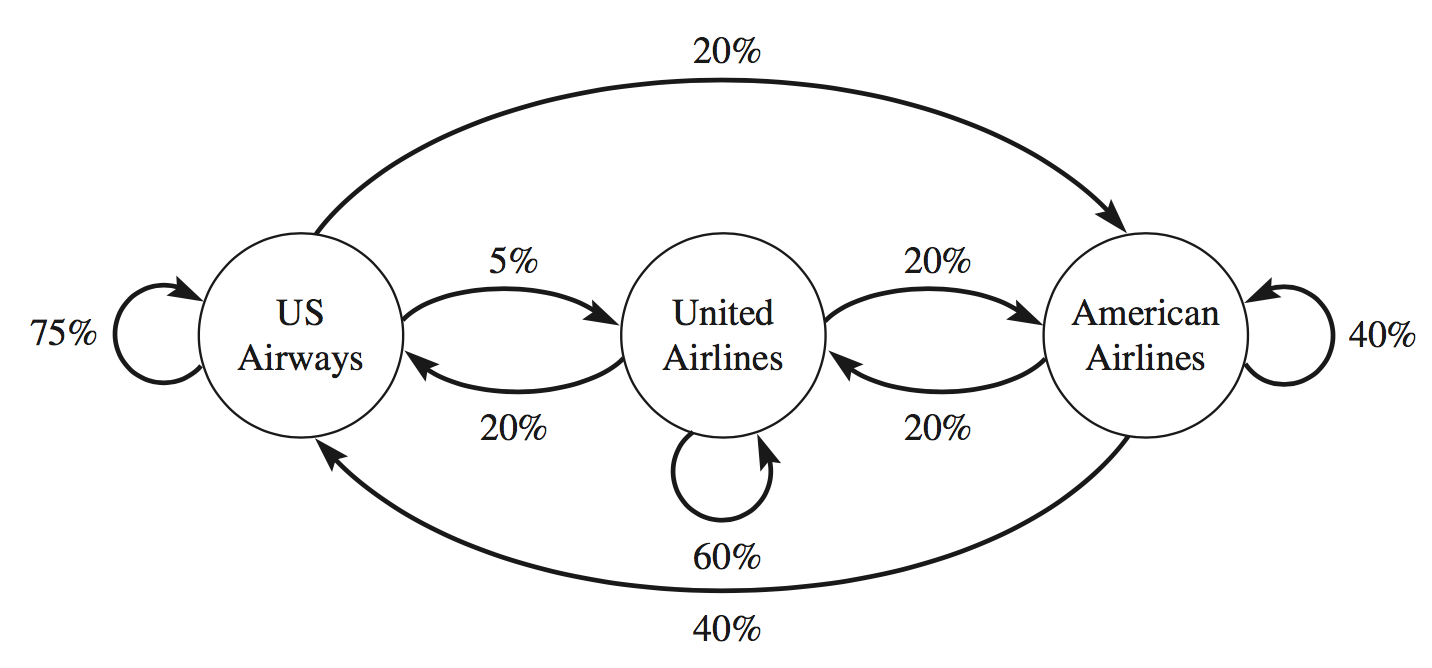
\includegraphics[width=0.6\textwidth,height=\textheight]{party.png}

\begin{itemize}
\tightlist
\item
  \(S_n =\) 第\(n\)个旅行周乘坐US Airways的旅客数
\item
  \(U_n =\) 第\(n\)个旅行周乘坐United Airlines的旅客数
\item
  \(A_n =\) 第\(n\)个旅行周乘坐American Airlines的旅客数
\end{itemize}
\end{frame}

\begin{frame}{差分方程组}
\phantomsection\label{ux5deeux5206ux65b9ux7a0bux7ec4-1}
\[
S_{n+1}=0.75S_n+0.20U_n+0.40A_n \\
U_{n+1}=0.05S_n+0.60U_n+0.20A_n \\
A_{n+1}=0.20S_n+0.20U_n+0.40A_n
\]

平衡点: \(S_{n+1}=S_n=S\), \(U_{n+1}=U_n=U\), \(A_{n+1}=A_n=A\):

\[
-0.25S+0.20U+0.40A=0 \\
0.05S-0.40U+0.20A=0 \\
0.20S+0.20U-0.60A=0
\]
\end{frame}

\begin{frame}{平衡点分析}
\phantomsection\label{ux5e73ux8861ux70b9ux5206ux6790-1}
\(S:U:A = 2.2221:0.7777694:1\)

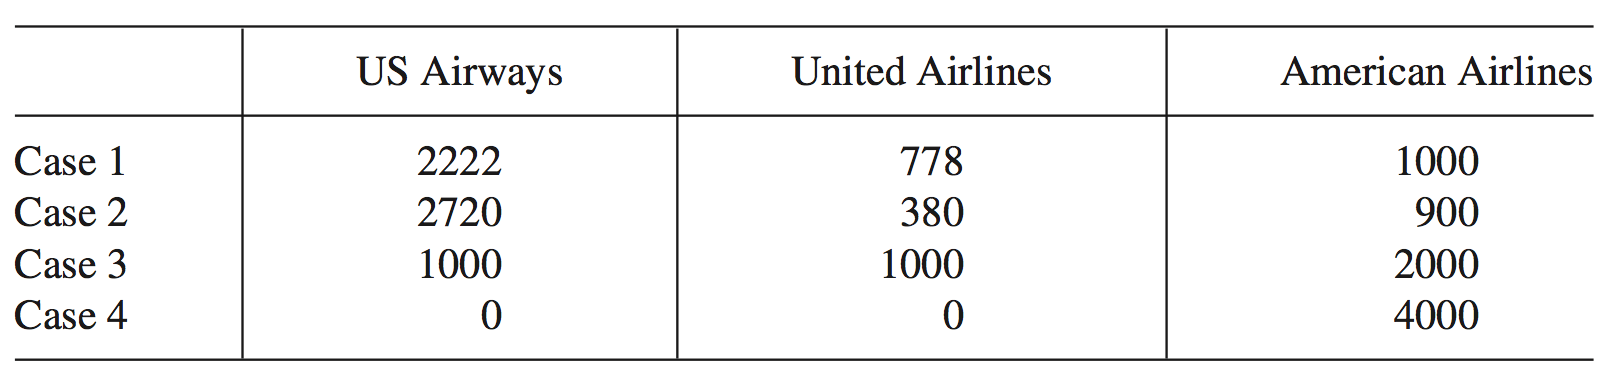
\includegraphics{party-case.png}
\end{frame}

\begin{frame}{情况1}
\phantomsection\label{ux60c5ux51b51-1}
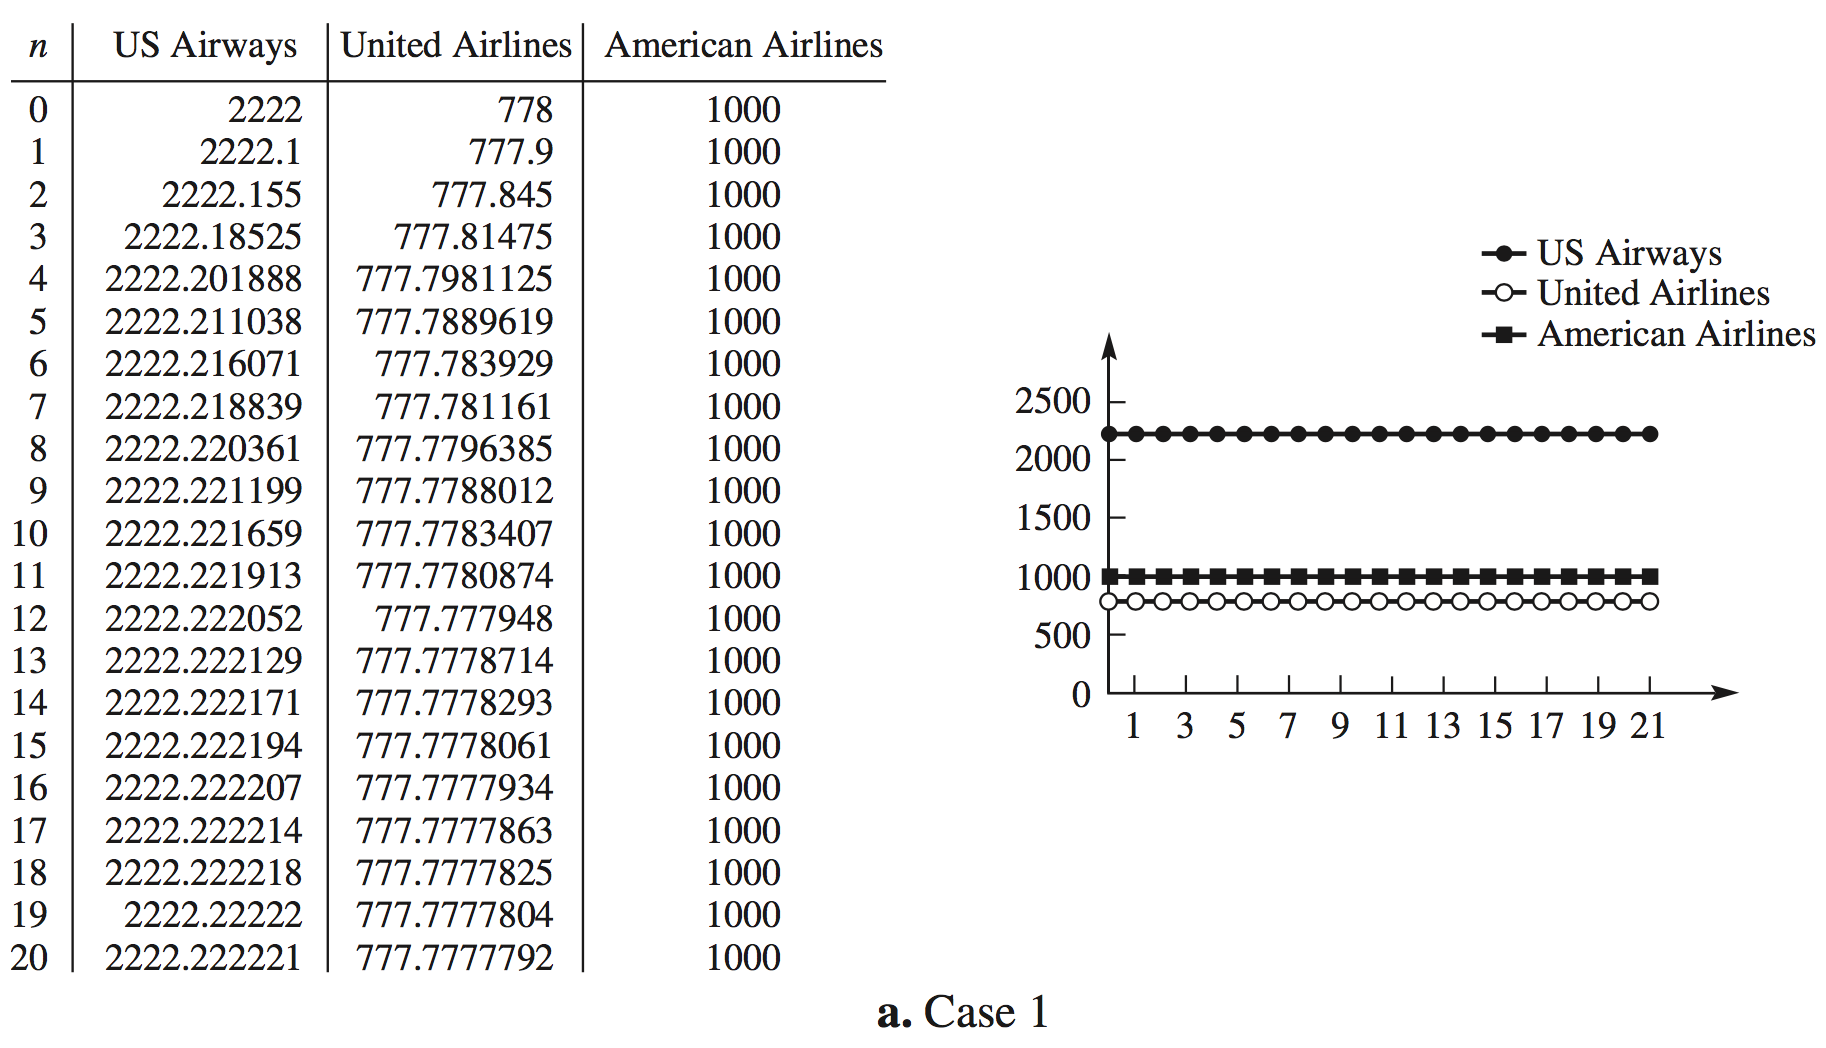
\includegraphics{party-1.png}
\end{frame}

\begin{frame}{情况2}
\phantomsection\label{ux60c5ux51b52-1}
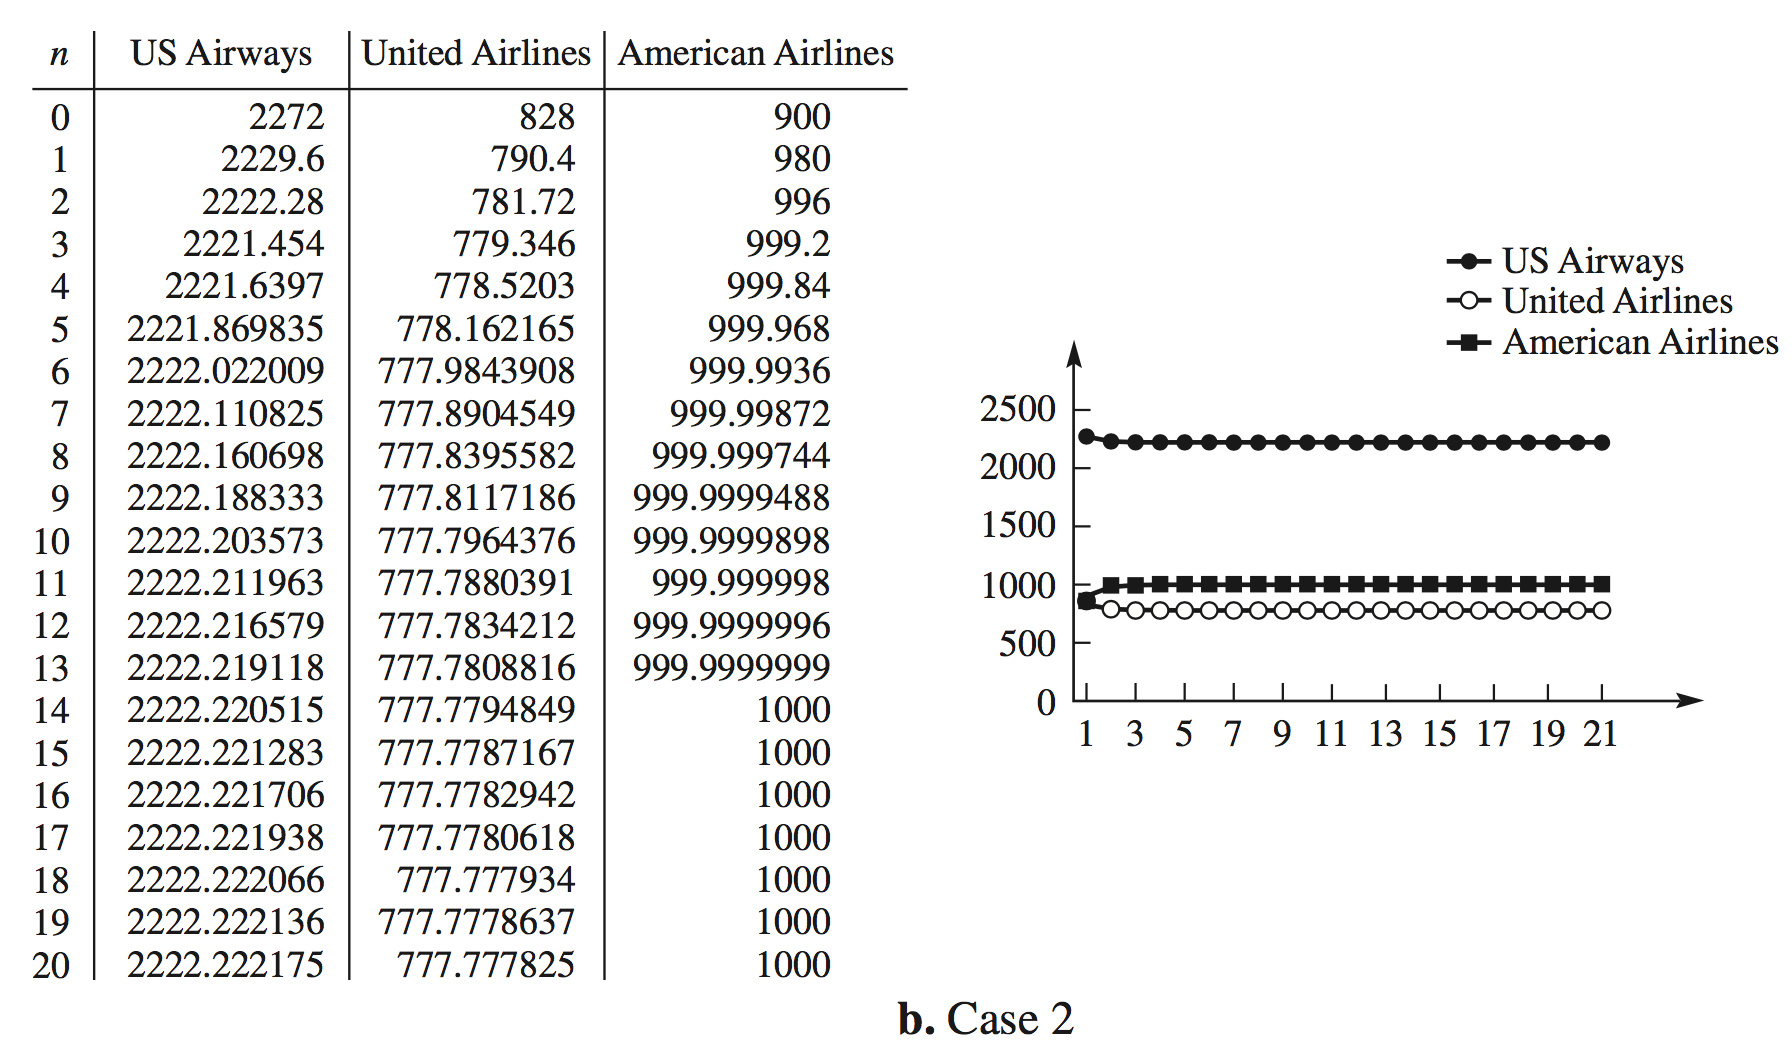
\includegraphics{party-2.png}
\end{frame}

\begin{frame}{情况3}
\phantomsection\label{ux60c5ux51b53-1}
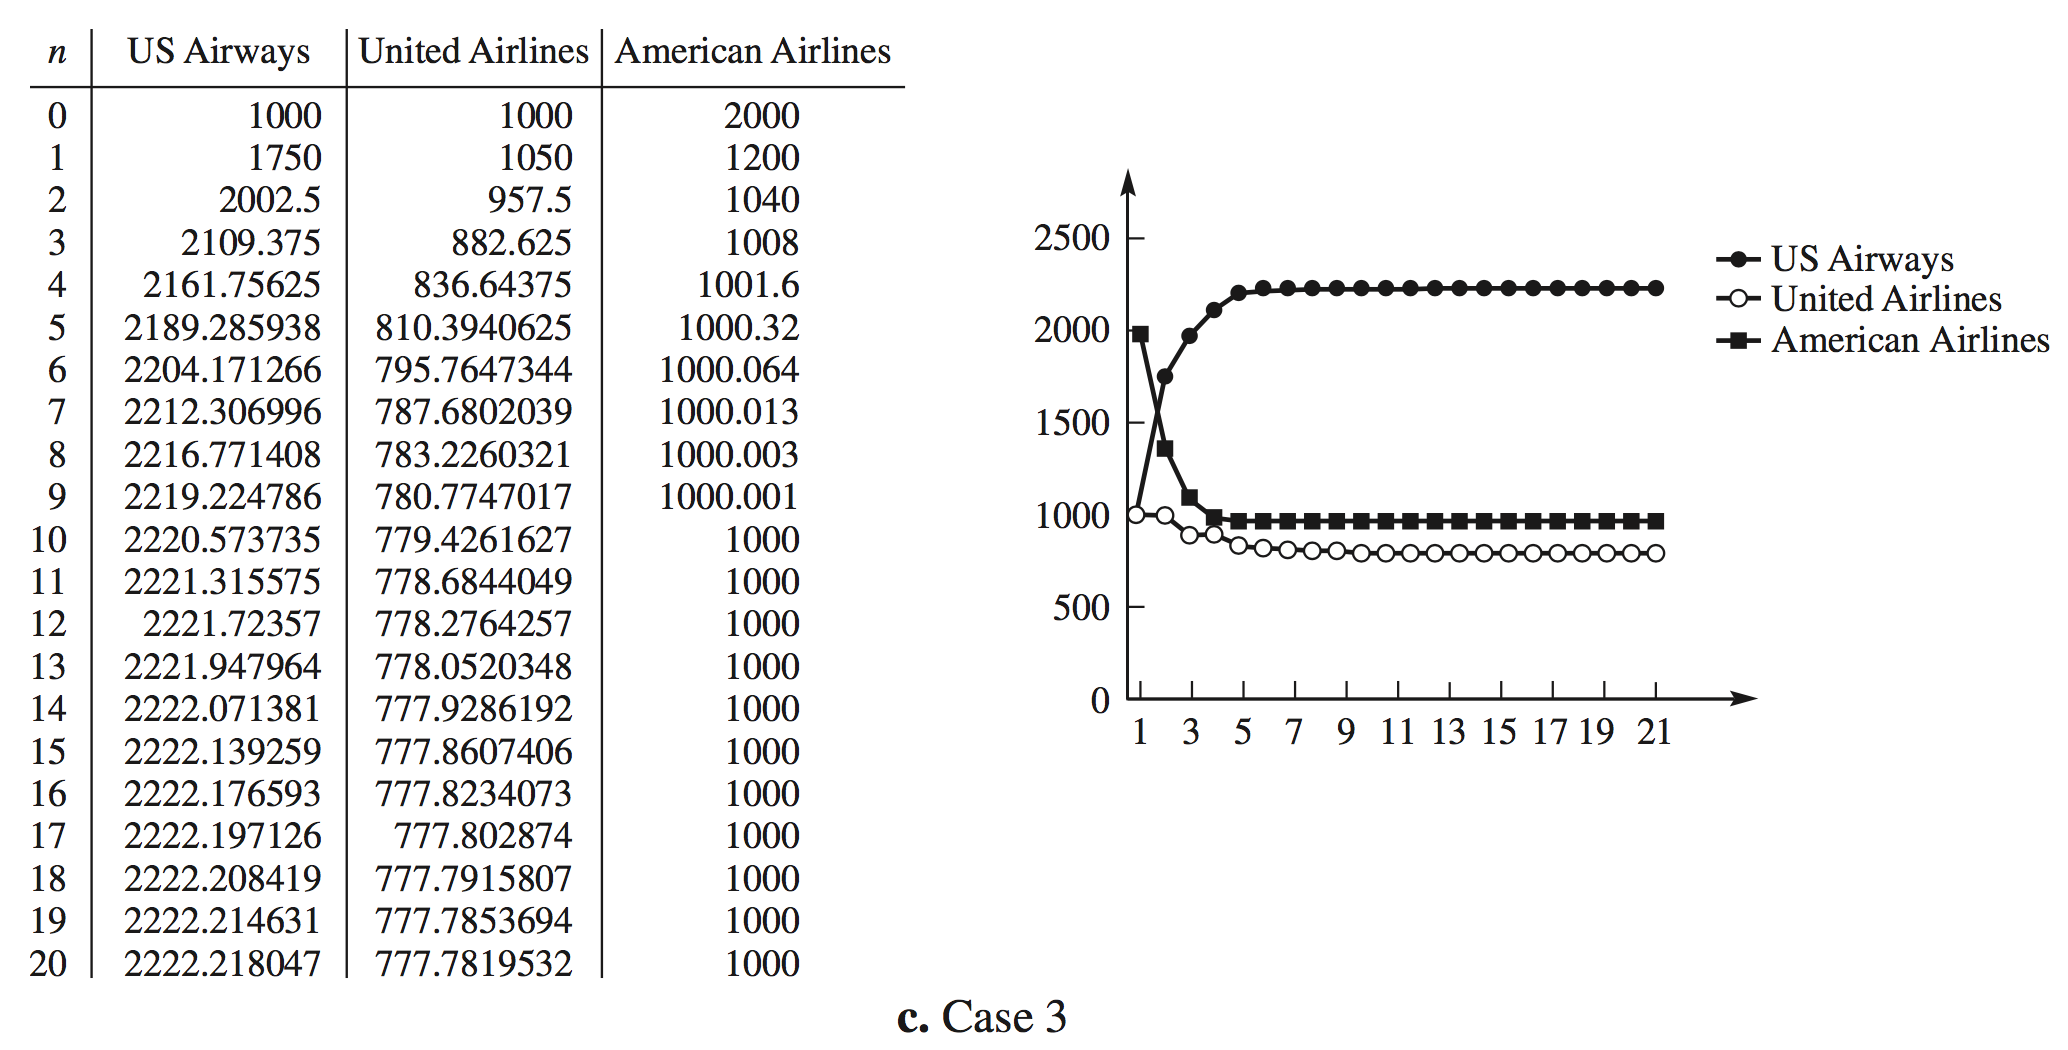
\includegraphics{party-3.png}
\end{frame}

\begin{frame}{情况4}
\phantomsection\label{ux60c5ux51b54}
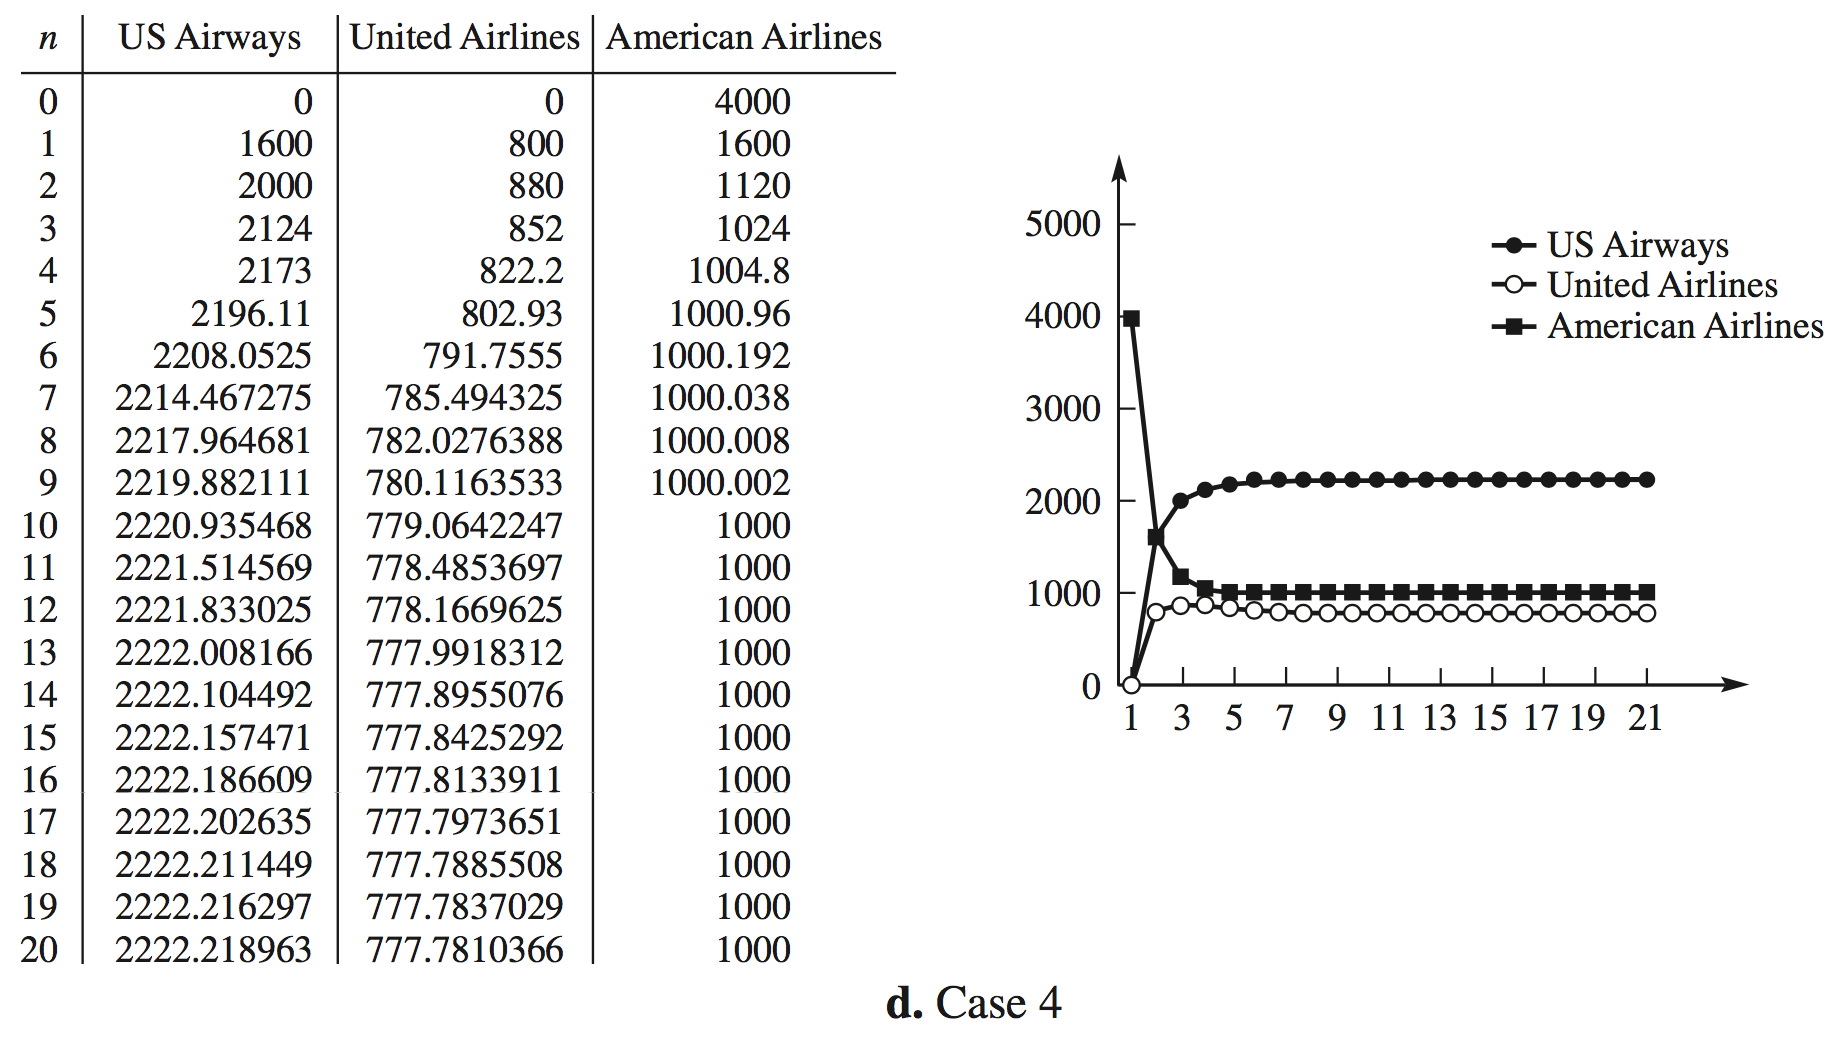
\includegraphics{party-4.png}
\end{frame}

\begin{frame}{总结}
\phantomsection\label{ux603bux7ed3}
系统相当稳定,即使刚开始没有人坐US Airways和United Airlines的旅客数.
\end{frame}




\end{document}
